\documentclass[twoside]{book}

% Packages required by doxygen
\usepackage{fixltx2e}
\usepackage{calc}
\usepackage{doxygen}
\usepackage[export]{adjustbox} % also loads graphicx
\usepackage{graphicx}
\usepackage[utf8]{inputenc}
\usepackage{makeidx}
\usepackage{multicol}
\usepackage{multirow}
\PassOptionsToPackage{warn}{textcomp}
\usepackage{textcomp}
\usepackage[nointegrals]{wasysym}
\usepackage[table]{xcolor}

% Font selection
\usepackage[T1]{fontenc}
\usepackage[scaled=.90]{helvet}
\usepackage{courier}
\usepackage{amssymb}
\usepackage{sectsty}
\renewcommand{\familydefault}{\sfdefault}
\allsectionsfont{%
  \fontseries{bc}\selectfont%
  \color{darkgray}%
}
\renewcommand{\DoxyLabelFont}{%
  \fontseries{bc}\selectfont%
  \color{darkgray}%
}
\newcommand{\+}{\discretionary{\mbox{\scriptsize$\hookleftarrow$}}{}{}}

% Page & text layout
\usepackage{geometry}
\geometry{%
  a4paper,%
  top=2.5cm,%
  bottom=2.5cm,%
  left=2.5cm,%
  right=2.5cm%
}
\tolerance=750
\hfuzz=15pt
\hbadness=750
\setlength{\emergencystretch}{15pt}
\setlength{\parindent}{0cm}
\setlength{\parskip}{3ex plus 2ex minus 2ex}
\makeatletter
\renewcommand{\paragraph}{%
  \@startsection{paragraph}{4}{0ex}{-1.0ex}{1.0ex}{%
    \normalfont\normalsize\bfseries\SS@parafont%
  }%
}
\renewcommand{\subparagraph}{%
  \@startsection{subparagraph}{5}{0ex}{-1.0ex}{1.0ex}{%
    \normalfont\normalsize\bfseries\SS@subparafont%
  }%
}
\makeatother

% Headers & footers
\usepackage{fancyhdr}
\pagestyle{fancyplain}
\fancyhead[LE]{\fancyplain{}{\bfseries\thepage}}
\fancyhead[CE]{\fancyplain{}{}}
\fancyhead[RE]{\fancyplain{}{\bfseries\leftmark}}
\fancyhead[LO]{\fancyplain{}{\bfseries\rightmark}}
\fancyhead[CO]{\fancyplain{}{}}
\fancyhead[RO]{\fancyplain{}{\bfseries\thepage}}
\fancyfoot[LE]{\fancyplain{}{}}
\fancyfoot[CE]{\fancyplain{}{}}
\fancyfoot[RE]{\fancyplain{}{\bfseries\scriptsize Generated by Doxygen }}
\fancyfoot[LO]{\fancyplain{}{\bfseries\scriptsize Generated by Doxygen }}
\fancyfoot[CO]{\fancyplain{}{}}
\fancyfoot[RO]{\fancyplain{}{}}
\renewcommand{\footrulewidth}{0.4pt}
\renewcommand{\chaptermark}[1]{%
  \markboth{#1}{}%
}
\renewcommand{\sectionmark}[1]{%
  \markright{\thesection\ #1}%
}

% Indices & bibliography
\usepackage{natbib}
\usepackage[titles]{tocloft}
\setcounter{tocdepth}{3}
\setcounter{secnumdepth}{5}
\makeindex

% Hyperlinks (required, but should be loaded last)
\usepackage{ifpdf}
\ifpdf
  \usepackage[pdftex,pagebackref=true]{hyperref}
\else
  \usepackage[ps2pdf,pagebackref=true]{hyperref}
\fi
\hypersetup{%
  colorlinks=true,%
  linkcolor=blue,%
  citecolor=blue,%
  unicode%
}

% Custom commands
\newcommand{\clearemptydoublepage}{%
  \newpage{\pagestyle{empty}\cleardoublepage}%
}

\usepackage{caption}
\captionsetup{labelsep=space,justification=centering,font={bf},singlelinecheck=off,skip=4pt,position=top}

%===== C O N T E N T S =====

\begin{document}

% Titlepage & ToC
\hypersetup{pageanchor=false,
             bookmarksnumbered=true,
             pdfencoding=unicode
            }
\pagenumbering{alph}
\begin{titlepage}
\vspace*{7cm}
\begin{center}%
{\Large Arcana\+Core Module }\\
\vspace*{1cm}
{\large Generated by Doxygen 1.8.14}\\
\end{center}
\end{titlepage}
\clearemptydoublepage
\pagenumbering{roman}
\tableofcontents
\clearemptydoublepage
\pagenumbering{arabic}
\hypersetup{pageanchor=true}

%--- Begin generated contents ---
\chapter{Hierarchical Index}
\section{Class Hierarchy}
This inheritance list is sorted roughly, but not completely, alphabetically\+:\begin{DoxyCompactList}
\item \contentsline{section}{Arcana\+:\+:Are\+Types\+Equal$<$ typename, typename $>$}{\pageref{struct_arcana_1_1_are_types_equal}}{}
\item \contentsline{section}{Arcana\+:\+:Are\+Types\+Equal$<$ A, A $>$}{\pageref{struct_arcana_1_1_are_types_equal_3_01_a_00_01_a_01_4}}{}
\item \contentsline{section}{Arcana\+:\+:Array$<$ Element\+Type $>$}{\pageref{class_arcana_1_1_array}}{}
\item \contentsline{section}{Arcana\+:\+:Array$<$ Arcana\+:\+:Event\+:\+:Data\+Point $>$}{\pageref{class_arcana_1_1_array}}{}
\item \contentsline{section}{Arcana\+:\+:Array$<$ Arcana\+:\+:Timeline\+:\+:Event\+Entry $>$}{\pageref{class_arcana_1_1_array}}{}
\item \contentsline{section}{Arcana\+:\+:Array$<$ std\+:\+:shared\+\_\+ptr$<$ Event\+Listener $>$ $>$}{\pageref{class_arcana_1_1_array}}{}
\item \contentsline{section}{Arcana\+:\+:Auto\+Profile}{\pageref{class_arcana_1_1_auto_profile}}{}
\item \contentsline{section}{Arcana\+:\+:Base\+Callback$<$ Return\+Value, Argument\+Types $>$}{\pageref{class_arcana_1_1_base_callback}}{}
\item \contentsline{section}{Arcana\+:\+:Event\+Handler\+:\+:Broadcast\+Result}{\pageref{class_arcana_1_1_event_handler_1_1_broadcast_result}}{}
\item \contentsline{section}{Arcana\+:\+:Event\+:\+:Data}{\pageref{class_arcana_1_1_event_1_1_data}}{}
\item \contentsline{section}{Arcana\+:\+:Event\+:\+:Data\+Point}{\pageref{struct_arcana_1_1_event_1_1_data_point}}{}
\item \contentsline{section}{Arcana\+:\+:Enable\+If$<$ Predicate, Result $>$}{\pageref{class_arcana_1_1_enable_if}}{}
\item \contentsline{section}{Arcana\+:\+:Enable\+If$<$ false, Result $>$}{\pageref{class_arcana_1_1_enable_if_3_01false_00_01_result_01_4}}{}
\item \contentsline{section}{Arcana\+:\+:Enable\+If$<$ true, Result $>$}{\pageref{class_arcana_1_1_enable_if_3_01true_00_01_result_01_4}}{}
\item \contentsline{section}{Arcana\+:\+:Timeline\+:\+:Event\+Entry}{\pageref{struct_arcana_1_1_timeline_1_1_event_entry}}{}
\item \contentsline{section}{Arcana\+:\+:Event\+Listener}{\pageref{class_arcana_1_1_event_listener}}{}
\item \contentsline{section}{Arcana\+:\+:Global\+Object\+ID}{\pageref{class_arcana_1_1_global_object_i_d}}{}
\item \contentsline{section}{Arcana\+:\+:Indexed\+Container\+Iterator$<$ Container\+Type, Element\+Type, Index\+Type $>$}{\pageref{class_arcana_1_1_indexed_container_iterator}}{}
\item \contentsline{section}{Arcana\+:\+:Is\+Base\+Of$<$ A, B $>$}{\pageref{struct_arcana_1_1_is_base_of}}{}
\item \contentsline{section}{Arcana\+:\+:Key\+Value\+Pair$<$ Key\+Type, Value\+Type $>$}{\pageref{struct_arcana_1_1_key_value_pair}}{}
\item \contentsline{section}{Arcana\+:\+:Memory}{\pageref{class_arcana_1_1_memory}}{}
\item \contentsline{section}{Arcana\+:\+:Memory\+Allocator}{\pageref{class_arcana_1_1_memory_allocator}}{}
\item \contentsline{section}{Arcana\+:\+:Message}{\pageref{class_arcana_1_1_message}}{}
\item \contentsline{section}{Arcana\+:\+:Module\+Interface}{\pageref{class_arcana_1_1_module_interface}}{}
\begin{DoxyCompactList}
\item \contentsline{section}{Arcana\+:\+:Core\+Module}{\pageref{class_arcana_1_1_core_module}}{}
\end{DoxyCompactList}
\item \contentsline{section}{Arcana\+:\+:Object}{\pageref{class_arcana_1_1_object}}{}
\begin{DoxyCompactList}
\item \contentsline{section}{Arcana\+:\+:Callback\+Instance$<$ Object\+Type, Return\+Value, Argument\+Types $>$}{\pageref{class_arcana_1_1_callback_instance}}{}
\item \contentsline{section}{Arcana\+:\+:Event}{\pageref{class_arcana_1_1_event}}{}
\begin{DoxyCompactList}
\item \contentsline{section}{Arcana\+:\+:Controller\+Connect\+Event}{\pageref{struct_arcana_1_1_controller_connect_event}}{}
\item \contentsline{section}{Arcana\+:\+:Key\+Event}{\pageref{class_arcana_1_1_key_event}}{}
\item \contentsline{section}{Arcana\+:\+:Mouse\+Event}{\pageref{class_arcana_1_1_mouse_event}}{}
\item \contentsline{section}{Arcana\+:\+:Window\+Closed\+Event}{\pageref{class_arcana_1_1_window_closed_event}}{}
\end{DoxyCompactList}
\item \contentsline{section}{Arcana\+:\+:Event\+Handler}{\pageref{class_arcana_1_1_event_handler}}{}
\item \contentsline{section}{Arcana\+:\+:Timeline}{\pageref{class_arcana_1_1_timeline}}{}
\item \contentsline{section}{Arcana\+:\+:Callback\+Instance$<$ void, Return\+Value, Argument\+Types... $>$}{\pageref{class_arcana_1_1_callback_instance}}{}
\begin{DoxyCompactList}
\item \contentsline{section}{Arcana\+:\+:Member\+Function\+Callback\+Instance$<$ Object\+Type, Return\+Value, Argument\+Types $>$}{\pageref{class_arcana_1_1_member_function_callback_instance}}{}
\item \contentsline{section}{Arcana\+:\+:Static\+Function\+Callback\+Instance$<$ Return\+Value, Argument\+Types $>$}{\pageref{class_arcana_1_1_static_function_callback_instance}}{}
\end{DoxyCompactList}
\end{DoxyCompactList}
\item \contentsline{section}{Arcana\+:\+:Object\+Destruction\+Manager}{\pageref{class_arcana_1_1_object_destruction_manager}}{}
\item \contentsline{section}{Arcana\+:\+:Profile\+Manager}{\pageref{class_arcana_1_1_profile_manager}}{}
\item \contentsline{section}{Arcana\+:\+:Remove\+Reference$<$ T $>$}{\pageref{struct_arcana_1_1_remove_reference}}{}
\item \contentsline{section}{Arcana\+:\+:Remove\+Reference$<$ T \&\& $>$}{\pageref{struct_arcana_1_1_remove_reference_3_01_t_01_6_6_01_4}}{}
\item \contentsline{section}{Arcana\+:\+:Remove\+Reference$<$ T \&$>$}{\pageref{struct_arcana_1_1_remove_reference_3_01_t_01_6_4}}{}
\item \contentsline{section}{Arcana\+:\+:Sleep}{\pageref{class_arcana_1_1_sleep}}{}
\item \contentsline{section}{Arcana\+:\+:Sleep\+Context}{\pageref{class_arcana_1_1_sleep_context}}{}
\item \contentsline{section}{Arcana\+:\+:Smart\+Ptr$<$ Object\+Type $>$}{\pageref{class_arcana_1_1_smart_ptr}}{}
\item \contentsline{section}{Arcana\+:\+:String}{\pageref{class_arcana_1_1_string}}{}
\item \contentsline{section}{Arcana\+:\+:Time}{\pageref{class_arcana_1_1_time}}{}
\item \contentsline{section}{Arcana\+:\+:Timer}{\pageref{class_arcana_1_1_timer}}{}
\item \contentsline{section}{Arcana\+:\+:Timer\+Context}{\pageref{class_arcana_1_1_timer_context}}{}
\item \contentsline{section}{Arcana\+:\+:Type}{\pageref{class_arcana_1_1_type}}{}
\item \contentsline{section}{Arcana\+:\+:Types}{\pageref{class_arcana_1_1_types}}{}
\item \contentsline{section}{Arcana\+:\+:Type\+Traits\+Base$<$ T $>$}{\pageref{struct_arcana_1_1_type_traits_base}}{}
\begin{DoxyCompactList}
\item \contentsline{section}{Arcana\+:\+:Type\+Traits$<$ T $>$}{\pageref{struct_arcana_1_1_type_traits}}{}
\end{DoxyCompactList}
\item \contentsline{section}{Arcana\+:\+:Memory\+Allocator\+:\+:Unknown\+Type}{\pageref{struct_arcana_1_1_memory_allocator_1_1_unknown_type}}{}
\end{DoxyCompactList}

\chapter{Class Index}
\section{Class List}
Here are the classes, structs, unions and interfaces with brief descriptions\+:\begin{DoxyCompactList}
\item\contentsline{section}{\mbox{\hyperlink{struct_arcana_1_1_are_types_equal}{Arcana\+::\+Are\+Types\+Equal$<$ typename, typename $>$}} }{\pageref{struct_arcana_1_1_are_types_equal}}{}
\item\contentsline{section}{\mbox{\hyperlink{struct_arcana_1_1_are_types_equal_3_01_a_00_01_a_01_4}{Arcana\+::\+Are\+Types\+Equal$<$ A, A $>$}} }{\pageref{struct_arcana_1_1_are_types_equal_3_01_a_00_01_a_01_4}}{}
\item\contentsline{section}{\mbox{\hyperlink{class_arcana_1_1_array}{Arcana\+::\+Array$<$ Element\+Type $>$}} \\*A dynamic array implementation }{\pageref{class_arcana_1_1_array}}{}
\item\contentsline{section}{\mbox{\hyperlink{class_arcana_1_1_auto_profile}{Arcana\+::\+Auto\+Profile}} \\*Times a section of code and stores the sample with the \mbox{\hyperlink{class_arcana_1_1_profile_manager}{Profile\+Manager}} }{\pageref{class_arcana_1_1_auto_profile}}{}
\item\contentsline{section}{\mbox{\hyperlink{class_arcana_1_1_base_callback}{Arcana\+::\+Base\+Callback$<$ Return\+Value, Argument\+Types $>$}} \\*A templated callback class }{\pageref{class_arcana_1_1_base_callback}}{}
\item\contentsline{section}{\mbox{\hyperlink{class_arcana_1_1_event_handler_1_1_broadcast_result}{Arcana\+::\+Event\+Handler\+::\+Broadcast\+Result}} \\*This class wraps a broadcast result code. It contains methods for easily checking success and getting code strings for debug printing }{\pageref{class_arcana_1_1_event_handler_1_1_broadcast_result}}{}
\item\contentsline{section}{\mbox{\hyperlink{class_arcana_1_1_callback_instance}{Arcana\+::\+Callback\+Instance$<$ Object\+Type, Return\+Value, Argument\+Types $>$}} \\*An instance of a callback }{\pageref{class_arcana_1_1_callback_instance}}{}
\item\contentsline{section}{\mbox{\hyperlink{struct_arcana_1_1_controller_connect_event}{Arcana\+::\+Controller\+Connect\+Event}} \\*Controller connection event }{\pageref{struct_arcana_1_1_controller_connect_event}}{}
\item\contentsline{section}{\mbox{\hyperlink{class_arcana_1_1_core_module}{Arcana\+::\+Core\+Module}} \\*The module interface for the Arcana\+Core module }{\pageref{class_arcana_1_1_core_module}}{}
\item\contentsline{section}{\mbox{\hyperlink{class_arcana_1_1_event_1_1_data}{Arcana\+::\+Event\+::\+Data}} \\*A wrapper for an array of data points }{\pageref{class_arcana_1_1_event_1_1_data}}{}
\item\contentsline{section}{\mbox{\hyperlink{struct_arcana_1_1_event_1_1_data_point}{Arcana\+::\+Event\+::\+Data\+Point}} \\*A struct that contains a name string and associated data }{\pageref{struct_arcana_1_1_event_1_1_data_point}}{}
\item\contentsline{section}{\mbox{\hyperlink{class_arcana_1_1_enable_if}{Arcana\+::\+Enable\+If$<$ Predicate, Result $>$}} }{\pageref{class_arcana_1_1_enable_if}}{}
\item\contentsline{section}{\mbox{\hyperlink{class_arcana_1_1_enable_if_3_01false_00_01_result_01_4}{Arcana\+::\+Enable\+If$<$ false, Result $>$}} }{\pageref{class_arcana_1_1_enable_if_3_01false_00_01_result_01_4}}{}
\item\contentsline{section}{\mbox{\hyperlink{class_arcana_1_1_enable_if_3_01true_00_01_result_01_4}{Arcana\+::\+Enable\+If$<$ true, Result $>$}} }{\pageref{class_arcana_1_1_enable_if_3_01true_00_01_result_01_4}}{}
\item\contentsline{section}{\mbox{\hyperlink{class_arcana_1_1_event}{Arcana\+::\+Event}} \\*\mbox{\hyperlink{class_arcana_1_1_event}{Event}} callback typedef }{\pageref{class_arcana_1_1_event}}{}
\item\contentsline{section}{\mbox{\hyperlink{struct_arcana_1_1_timeline_1_1_event_entry}{Arcana\+::\+Timeline\+::\+Event\+Entry}} \\*An event entry }{\pageref{struct_arcana_1_1_timeline_1_1_event_entry}}{}
\item\contentsline{section}{\mbox{\hyperlink{class_arcana_1_1_event_handler}{Arcana\+::\+Event\+Handler}} \\*Main class for broadcasting events }{\pageref{class_arcana_1_1_event_handler}}{}
\item\contentsline{section}{\mbox{\hyperlink{class_arcana_1_1_event_listener}{Arcana\+::\+Event\+Listener}} \\*An interface for processing events }{\pageref{class_arcana_1_1_event_listener}}{}
\item\contentsline{section}{\mbox{\hyperlink{class_arcana_1_1_global_object_i_d}{Arcana\+::\+Global\+Object\+ID}} \\*A global object id }{\pageref{class_arcana_1_1_global_object_i_d}}{}
\item\contentsline{section}{\mbox{\hyperlink{class_arcana_1_1_indexed_container_iterator}{Arcana\+::\+Indexed\+Container\+Iterator$<$ Container\+Type, Element\+Type, Index\+Type $>$}} \\*Iterator for custom Arcana\+Engine containers }{\pageref{class_arcana_1_1_indexed_container_iterator}}{}
\item\contentsline{section}{\mbox{\hyperlink{struct_arcana_1_1_is_base_of}{Arcana\+::\+Is\+Base\+Of$<$ A, B $>$}} }{\pageref{struct_arcana_1_1_is_base_of}}{}
\item\contentsline{section}{\mbox{\hyperlink{class_arcana_1_1_key_event}{Arcana\+::\+Key\+Event}} \\*\mbox{\hyperlink{class_arcana_1_1_event}{Event}} broadcasted on key presses/releases }{\pageref{class_arcana_1_1_key_event}}{}
\item\contentsline{section}{\mbox{\hyperlink{struct_arcana_1_1_key_value_pair}{Arcana\+::\+Key\+Value\+Pair$<$ Key\+Type, Value\+Type $>$}} \\*Key/value pairs that are easy to use with custom containers. This class acts the same as the standard pair }{\pageref{struct_arcana_1_1_key_value_pair}}{}
\item\contentsline{section}{\mbox{\hyperlink{class_arcana_1_1_member_function_callback_instance}{Arcana\+::\+Member\+Function\+Callback\+Instance$<$ Object\+Type, Return\+Value, Argument\+Types $>$}} \\*Callback instance wrapping a member function pointer }{\pageref{class_arcana_1_1_member_function_callback_instance}}{}
\item\contentsline{section}{\mbox{\hyperlink{class_arcana_1_1_memory}{Arcana\+::\+Memory}} \\*Handles memory allocations. This class wraps platform-\/specific memory operations and provides simple memory management methods }{\pageref{class_arcana_1_1_memory}}{}
\item\contentsline{section}{\mbox{\hyperlink{class_arcana_1_1_memory_allocator}{Arcana\+::\+Memory\+Allocator}} }{\pageref{class_arcana_1_1_memory_allocator}}{}
\item\contentsline{section}{\mbox{\hyperlink{class_arcana_1_1_message}{Arcana\+::\+Message}} \\*This class manages the lifetime of an \mbox{\hyperlink{class_arcana_1_1_event}{Event}} pointer }{\pageref{class_arcana_1_1_message}}{}
\item\contentsline{section}{\mbox{\hyperlink{class_arcana_1_1_module_interface}{Arcana\+::\+Module\+Interface}} \\*Interface for Engine and Game modules }{\pageref{class_arcana_1_1_module_interface}}{}
\item\contentsline{section}{\mbox{\hyperlink{class_arcana_1_1_mouse_event}{Arcana\+::\+Mouse\+Event}} \\*\mbox{\hyperlink{class_arcana_1_1_event}{Event}} broadcasted on mouse presses/releases/movement/etc }{\pageref{class_arcana_1_1_mouse_event}}{}
\item\contentsline{section}{\mbox{\hyperlink{class_arcana_1_1_object}{Arcana\+::\+Object}} \\*The base class for all core classes }{\pageref{class_arcana_1_1_object}}{}
\item\contentsline{section}{\mbox{\hyperlink{class_arcana_1_1_object_destruction_manager}{Arcana\+::\+Object\+Destruction\+Manager}} \\*Manages automatic garbage collection }{\pageref{class_arcana_1_1_object_destruction_manager}}{}
\item\contentsline{section}{\mbox{\hyperlink{class_arcana_1_1_profile_manager}{Arcana\+::\+Profile\+Manager}} \\*Manager for profile samples }{\pageref{class_arcana_1_1_profile_manager}}{}
\item\contentsline{section}{\mbox{\hyperlink{struct_arcana_1_1_remove_reference}{Arcana\+::\+Remove\+Reference$<$ T $>$}} }{\pageref{struct_arcana_1_1_remove_reference}}{}
\item\contentsline{section}{\mbox{\hyperlink{struct_arcana_1_1_remove_reference_3_01_t_01_6_6_01_4}{Arcana\+::\+Remove\+Reference$<$ T \&\& $>$}} }{\pageref{struct_arcana_1_1_remove_reference_3_01_t_01_6_6_01_4}}{}
\item\contentsline{section}{\mbox{\hyperlink{struct_arcana_1_1_remove_reference_3_01_t_01_6_4}{Arcana\+::\+Remove\+Reference$<$ T \&$>$}} }{\pageref{struct_arcana_1_1_remove_reference_3_01_t_01_6_4}}{}
\item\contentsline{section}{\mbox{\hyperlink{class_arcana_1_1_sleep}{Arcana\+::\+Sleep}} \\*Platform-\/independent sleep implementation }{\pageref{class_arcana_1_1_sleep}}{}
\item\contentsline{section}{\mbox{\hyperlink{class_arcana_1_1_sleep_context}{Arcana\+::\+Sleep\+Context}} \\*Windows sleep implementation }{\pageref{class_arcana_1_1_sleep_context}}{}
\item\contentsline{section}{\mbox{\hyperlink{class_arcana_1_1_smart_ptr}{Arcana\+::\+Smart\+Ptr$<$ Object\+Type $>$}} \\*A templated smart pointer implementation }{\pageref{class_arcana_1_1_smart_ptr}}{}
\item\contentsline{section}{\mbox{\hyperlink{class_arcana_1_1_static_function_callback_instance}{Arcana\+::\+Static\+Function\+Callback\+Instance$<$ Return\+Value, Argument\+Types $>$}} }{\pageref{class_arcana_1_1_static_function_callback_instance}}{}
\item\contentsline{section}{\mbox{\hyperlink{class_arcana_1_1_string}{Arcana\+::\+String}} }{\pageref{class_arcana_1_1_string}}{}
\item\contentsline{section}{\mbox{\hyperlink{class_arcana_1_1_time}{Arcana\+::\+Time}} \\*Class for wrapping a time duration }{\pageref{class_arcana_1_1_time}}{}
\item\contentsline{section}{\mbox{\hyperlink{class_arcana_1_1_timeline}{Arcana\+::\+Timeline}} \\*This class manages a timeline }{\pageref{class_arcana_1_1_timeline}}{}
\item\contentsline{section}{\mbox{\hyperlink{class_arcana_1_1_timer}{Arcana\+::\+Timer}} \\*A basic timer }{\pageref{class_arcana_1_1_timer}}{}
\item\contentsline{section}{\mbox{\hyperlink{class_arcana_1_1_timer_context}{Arcana\+::\+Timer\+Context}} \\*Windows timer implementation }{\pageref{class_arcana_1_1_timer_context}}{}
\item\contentsline{section}{\mbox{\hyperlink{class_arcana_1_1_type}{Arcana\+::\+Type}} }{\pageref{class_arcana_1_1_type}}{}
\item\contentsline{section}{\mbox{\hyperlink{class_arcana_1_1_types}{Arcana\+::\+Types}} }{\pageref{class_arcana_1_1_types}}{}
\item\contentsline{section}{\mbox{\hyperlink{struct_arcana_1_1_type_traits}{Arcana\+::\+Type\+Traits$<$ T $>$}} }{\pageref{struct_arcana_1_1_type_traits}}{}
\item\contentsline{section}{\mbox{\hyperlink{struct_arcana_1_1_type_traits_base}{Arcana\+::\+Type\+Traits\+Base$<$ T $>$}} }{\pageref{struct_arcana_1_1_type_traits_base}}{}
\item\contentsline{section}{\mbox{\hyperlink{struct_arcana_1_1_memory_allocator_1_1_unknown_type}{Arcana\+::\+Memory\+Allocator\+::\+Unknown\+Type}} }{\pageref{struct_arcana_1_1_memory_allocator_1_1_unknown_type}}{}
\item\contentsline{section}{\mbox{\hyperlink{class_arcana_1_1_window_closed_event}{Arcana\+::\+Window\+Closed\+Event}} \\*\mbox{\hyperlink{class_arcana_1_1_event}{Event}} broadcasted on window close }{\pageref{class_arcana_1_1_window_closed_event}}{}
\end{DoxyCompactList}

\chapter{Class Documentation}
\hypertarget{struct_arcana_1_1_are_types_equal}{}\section{Arcana\+:\+:Are\+Types\+Equal$<$ typename, typename $>$ Struct Template Reference}
\label{struct_arcana_1_1_are_types_equal}\index{Arcana\+::\+Are\+Types\+Equal$<$ typename, typename $>$@{Arcana\+::\+Are\+Types\+Equal$<$ typename, typename $>$}}
\subsection*{Public Types}
\begin{DoxyCompactItemize}
\item 
\mbox{\Hypertarget{struct_arcana_1_1_are_types_equal_a41316d5fe9a645a3f71a6d1b2d9a985b}\label{struct_arcana_1_1_are_types_equal_a41316d5fe9a645a3f71a6d1b2d9a985b}} 
enum \{ {\bfseries Value} = false
 \}
\end{DoxyCompactItemize}


The documentation for this struct was generated from the following file\+:\begin{DoxyCompactItemize}
\item 
Type\+Traits.\+h\end{DoxyCompactItemize}

\hypertarget{struct_arcana_1_1_are_types_equal_3_01_a_00_01_a_01_4}{}\section{Arcana\+:\+:Are\+Types\+Equal$<$ A, A $>$ Struct Template Reference}
\label{struct_arcana_1_1_are_types_equal_3_01_a_00_01_a_01_4}\index{Arcana\+::\+Are\+Types\+Equal$<$ A, A $>$@{Arcana\+::\+Are\+Types\+Equal$<$ A, A $>$}}
\subsection*{Public Types}
\begin{DoxyCompactItemize}
\item 
\mbox{\Hypertarget{struct_arcana_1_1_are_types_equal_3_01_a_00_01_a_01_4_a8b24f46752d73cfdb5eb9b5e300702cd}\label{struct_arcana_1_1_are_types_equal_3_01_a_00_01_a_01_4_a8b24f46752d73cfdb5eb9b5e300702cd}} 
enum \{ {\bfseries Value} = true
 \}
\end{DoxyCompactItemize}


The documentation for this struct was generated from the following file\+:\begin{DoxyCompactItemize}
\item 
Type\+Traits.\+h\end{DoxyCompactItemize}

\hypertarget{class_arcana_1_1_array}{}\section{Arcana\+:\+:Array$<$ Element\+Type $>$ Class Template Reference}
\label{class_arcana_1_1_array}\index{Arcana\+::\+Array$<$ Element\+Type $>$@{Arcana\+::\+Array$<$ Element\+Type $>$}}


A dynamic array implementation.  




{\ttfamily \#include $<$Array.\+h$>$}

\subsection*{Public Types}
\begin{DoxyCompactItemize}
\item 
\mbox{\Hypertarget{class_arcana_1_1_array_a86a41fae7e14a94fd085bfffcc40e3b1}\label{class_arcana_1_1_array_a86a41fae7e14a94fd085bfffcc40e3b1}} 
typedef \mbox{\hyperlink{class_arcana_1_1_indexed_container_iterator}{Indexed\+Container\+Iterator}}$<$ \mbox{\hyperlink{class_arcana_1_1_array}{Array}}, Element\+Type, int32 $>$ {\bfseries Iterator}
\item 
\mbox{\Hypertarget{class_arcana_1_1_array_ad04b27e3627e03c3771db375bd68bae7}\label{class_arcana_1_1_array_ad04b27e3627e03c3771db375bd68bae7}} 
typedef \mbox{\hyperlink{class_arcana_1_1_indexed_container_iterator}{Indexed\+Container\+Iterator}}$<$ const \mbox{\hyperlink{class_arcana_1_1_array}{Array}}, const Element\+Type, int32 $>$ {\bfseries Const\+Iterator}
\end{DoxyCompactItemize}
\subsection*{Public Member Functions}
\begin{DoxyCompactItemize}
\item 
\mbox{\Hypertarget{class_arcana_1_1_array_addac09b78eaea1ef29ccc06320478eca}\label{class_arcana_1_1_array_addac09b78eaea1ef29ccc06320478eca}} 
\mbox{\hyperlink{class_arcana_1_1_array_addac09b78eaea1ef29ccc06320478eca}{Array}} ()
\begin{DoxyCompactList}\small\item\em Default array constructor. \end{DoxyCompactList}\item 
\mbox{\Hypertarget{class_arcana_1_1_array_a86acb91bd19f5c18d48ddf1e76b004c1}\label{class_arcana_1_1_array_a86acb91bd19f5c18d48ddf1e76b004c1}} 
\mbox{\hyperlink{class_arcana_1_1_array_a86acb91bd19f5c18d48ddf1e76b004c1}{Array}} (const \mbox{\hyperlink{class_arcana_1_1_array}{Array}}$<$ Element\+Type $>$ \&other)
\begin{DoxyCompactList}\small\item\em \mbox{\hyperlink{class_arcana_1_1_array}{Array}} copy constructor. \end{DoxyCompactList}\item 
\mbox{\Hypertarget{class_arcana_1_1_array_a9b81cbd9e686a53c8d307e35740d981a}\label{class_arcana_1_1_array_a9b81cbd9e686a53c8d307e35740d981a}} 
\mbox{\hyperlink{class_arcana_1_1_array_a9b81cbd9e686a53c8d307e35740d981a}{Array}} (const \mbox{\hyperlink{class_arcana_1_1_array}{Array}}$<$ Element\+Type $>$ \&other, int32 extra\+Slack)
\begin{DoxyCompactList}\small\item\em \mbox{\hyperlink{class_arcana_1_1_array}{Array}} copy constructor with slack parameter. Copies array normally, but adds specified extra slack. \end{DoxyCompactList}\item 
\mbox{\Hypertarget{class_arcana_1_1_array_ad25159a8deca52693caaf9dd39b61fd3}\label{class_arcana_1_1_array_ad25159a8deca52693caaf9dd39b61fd3}} 
\mbox{\hyperlink{class_arcana_1_1_array}{Array}}$<$ Element\+Type $>$ \& \mbox{\hyperlink{class_arcana_1_1_array_ad25159a8deca52693caaf9dd39b61fd3}{operator=}} (const \mbox{\hyperlink{class_arcana_1_1_array}{Array}}$<$ Element\+Type $>$ \&other)
\begin{DoxyCompactList}\small\item\em \mbox{\hyperlink{class_arcana_1_1_array}{Array}} assignment operator. \end{DoxyCompactList}\item 
\mbox{\Hypertarget{class_arcana_1_1_array_ab9ddb391868e9e4b8b8dba44778ff9e0}\label{class_arcana_1_1_array_ab9ddb391868e9e4b8b8dba44778ff9e0}} 
\mbox{\hyperlink{class_arcana_1_1_array_ab9ddb391868e9e4b8b8dba44778ff9e0}{Array}} (\mbox{\hyperlink{class_arcana_1_1_array}{Array}}$<$ Element\+Type $>$ \&\&other)
\begin{DoxyCompactList}\small\item\em \mbox{\hyperlink{class_arcana_1_1_array}{Array}} move constructor. \end{DoxyCompactList}\item 
\mbox{\Hypertarget{class_arcana_1_1_array_adae8ba60220ecde6bf7f53d2ff80ae90}\label{class_arcana_1_1_array_adae8ba60220ecde6bf7f53d2ff80ae90}} 
\mbox{\hyperlink{class_arcana_1_1_array}{Array}}$<$ Element\+Type $>$ \& \mbox{\hyperlink{class_arcana_1_1_array_adae8ba60220ecde6bf7f53d2ff80ae90}{operator=}} (\mbox{\hyperlink{class_arcana_1_1_array}{Array}}$<$ Element\+Type $>$ \&\&other)
\begin{DoxyCompactList}\small\item\em \mbox{\hyperlink{class_arcana_1_1_array}{Array}} move assignment operator. \end{DoxyCompactList}\item 
\mbox{\Hypertarget{class_arcana_1_1_array_a9cc19e98ee2fc944c0c5aab64b1ae3c6}\label{class_arcana_1_1_array_a9cc19e98ee2fc944c0c5aab64b1ae3c6}} 
\mbox{\hyperlink{class_arcana_1_1_array_a9cc19e98ee2fc944c0c5aab64b1ae3c6}{$\sim$\+Array}} ()
\begin{DoxyCompactList}\small\item\em \mbox{\hyperlink{class_arcana_1_1_array}{Array}} destructor. Frees allocated memory. \end{DoxyCompactList}\item 
\mbox{\Hypertarget{class_arcana_1_1_array_a5cdee51f03c8987970f841bbe07117d2}\label{class_arcana_1_1_array_a5cdee51f03c8987970f841bbe07117d2}} 
Element\+Type $\ast$ \mbox{\hyperlink{class_arcana_1_1_array_a5cdee51f03c8987970f841bbe07117d2}{get\+Data}} ()
\begin{DoxyCompactList}\small\item\em Returns a raw pointer to the array data. \end{DoxyCompactList}\item 
\mbox{\Hypertarget{class_arcana_1_1_array_a348d34e37a8257e4d9384740a174ab9e}\label{class_arcana_1_1_array_a348d34e37a8257e4d9384740a174ab9e}} 
const Element\+Type $\ast$ \mbox{\hyperlink{class_arcana_1_1_array_a348d34e37a8257e4d9384740a174ab9e}{get\+Data}} () const
\begin{DoxyCompactList}\small\item\em Returns a const pointer to the array data. \end{DoxyCompactList}\item 
\mbox{\Hypertarget{class_arcana_1_1_array_a027f9a11ecfa2c31be32a9746e9ff0d2}\label{class_arcana_1_1_array_a027f9a11ecfa2c31be32a9746e9ff0d2}} 
uint32 \mbox{\hyperlink{class_arcana_1_1_array_a027f9a11ecfa2c31be32a9746e9ff0d2}{get\+Type\+Size}} () const
\begin{DoxyCompactList}\small\item\em Returns the size in bytes of the element type. \end{DoxyCompactList}\item 
\mbox{\Hypertarget{class_arcana_1_1_array_a3dc8ca21eebaaaab6a3bc9fe3243dc15}\label{class_arcana_1_1_array_a3dc8ca21eebaaaab6a3bc9fe3243dc15}} 
uint32 \mbox{\hyperlink{class_arcana_1_1_array_a3dc8ca21eebaaaab6a3bc9fe3243dc15}{get\+Allocated\+Size}} () const
\begin{DoxyCompactList}\small\item\em Returns total size in bytes allocated to this array by the \mbox{\hyperlink{class_arcana_1_1_memory_allocator}{Memory\+Allocator}}. \end{DoxyCompactList}\item 
\mbox{\Hypertarget{class_arcana_1_1_array_ac0ffb30e2385e0154b9e50a29ad557cb}\label{class_arcana_1_1_array_ac0ffb30e2385e0154b9e50a29ad557cb}} 
int32 \mbox{\hyperlink{class_arcana_1_1_array_ac0ffb30e2385e0154b9e50a29ad557cb}{get\+Slack}} () const
\begin{DoxyCompactList}\small\item\em Returns the amount of slack allocated. \end{DoxyCompactList}\item 
\mbox{\Hypertarget{class_arcana_1_1_array_aa7971fa123cf15e7466c6795a1d04ed6}\label{class_arcana_1_1_array_aa7971fa123cf15e7466c6795a1d04ed6}} 
void \mbox{\hyperlink{class_arcana_1_1_array_aa7971fa123cf15e7466c6795a1d04ed6}{check\+Invariants}} () const
\begin{DoxyCompactList}\small\item\em Ensures a non-\/negative array size and a max size greater than or equal to the current size. \end{DoxyCompactList}\item 
\mbox{\Hypertarget{class_arcana_1_1_array_ab457f2db9ded37cbb2db24591eaf173d}\label{class_arcana_1_1_array_ab457f2db9ded37cbb2db24591eaf173d}} 
void \mbox{\hyperlink{class_arcana_1_1_array_ab457f2db9ded37cbb2db24591eaf173d}{range\+Check}} (int32 index) const
\begin{DoxyCompactList}\small\item\em Ensures an index is non-\/negative and less than the array size. \end{DoxyCompactList}\item 
\mbox{\Hypertarget{class_arcana_1_1_array_a0b1c26013b63c374bc9e980e364d6e14}\label{class_arcana_1_1_array_a0b1c26013b63c374bc9e980e364d6e14}} 
bool \mbox{\hyperlink{class_arcana_1_1_array_a0b1c26013b63c374bc9e980e364d6e14}{is\+Valid\+Index}} (int32 index) const
\begin{DoxyCompactList}\small\item\em Return true if the index is non-\/negative and less than the array size. \end{DoxyCompactList}\item 
\mbox{\Hypertarget{class_arcana_1_1_array_a546fb9ca70679870ad1989969226c36f}\label{class_arcana_1_1_array_a546fb9ca70679870ad1989969226c36f}} 
int32 \mbox{\hyperlink{class_arcana_1_1_array_a546fb9ca70679870ad1989969226c36f}{size}} () const
\begin{DoxyCompactList}\small\item\em Returns the number of elements in the array. \end{DoxyCompactList}\item 
\mbox{\Hypertarget{class_arcana_1_1_array_a1dc82d25f171e88b12c4f6a2c3ca0a86}\label{class_arcana_1_1_array_a1dc82d25f171e88b12c4f6a2c3ca0a86}} 
int32() \mbox{\hyperlink{class_arcana_1_1_array_a1dc82d25f171e88b12c4f6a2c3ca0a86}{max}} () const
\begin{DoxyCompactList}\small\item\em Returns the maximum number of elements that can be added without reallocating. \end{DoxyCompactList}\item 
\mbox{\Hypertarget{class_arcana_1_1_array_a3cb44835c75d9e1e3bce3bae208ec33e}\label{class_arcana_1_1_array_a3cb44835c75d9e1e3bce3bae208ec33e}} 
Element\+Type \& \mbox{\hyperlink{class_arcana_1_1_array_a3cb44835c75d9e1e3bce3bae208ec33e}{operator\mbox{[}$\,$\mbox{]}}} (int32 index)
\begin{DoxyCompactList}\small\item\em \mbox{\hyperlink{class_arcana_1_1_array}{Array}} offset operator. Returns a reference to the element at the specified index. \end{DoxyCompactList}\item 
\mbox{\Hypertarget{class_arcana_1_1_array_ac04751f78e6846fa55a633e3acc96e23}\label{class_arcana_1_1_array_ac04751f78e6846fa55a633e3acc96e23}} 
const Element\+Type \& \mbox{\hyperlink{class_arcana_1_1_array_ac04751f78e6846fa55a633e3acc96e23}{operator\mbox{[}$\,$\mbox{]}}} (int32 index) const
\begin{DoxyCompactList}\small\item\em \mbox{\hyperlink{class_arcana_1_1_array}{Array}} offset operator. Returns a const reference to the element at the specified index. \end{DoxyCompactList}\item 
\mbox{\Hypertarget{class_arcana_1_1_array_a952855bbeb0b73ee905e088e5bd02082}\label{class_arcana_1_1_array_a952855bbeb0b73ee905e088e5bd02082}} 
Element\+Type \mbox{\hyperlink{class_arcana_1_1_array_a952855bbeb0b73ee905e088e5bd02082}{pop}} (bool allow\+Shrinking=true)
\begin{DoxyCompactList}\small\item\em Removes the last element in the array. If \textquotesingle{}allow\+Shrinking\textquotesingle{} is true, the \mbox{\hyperlink{class_arcana_1_1_memory_allocator}{Memory\+Allocator}} can decrease the array\textquotesingle{}s allocated memory. \end{DoxyCompactList}\item 
\mbox{\Hypertarget{class_arcana_1_1_array_a0d1872dfb564625c1eb451112b14023e}\label{class_arcana_1_1_array_a0d1872dfb564625c1eb451112b14023e}} 
void \mbox{\hyperlink{class_arcana_1_1_array_a0d1872dfb564625c1eb451112b14023e}{push}} (Element\+Type \&\&element)
\begin{DoxyCompactList}\small\item\em Inserts an element at the end of the array. \end{DoxyCompactList}\item 
\mbox{\Hypertarget{class_arcana_1_1_array_aa1c62a1fcad8d75472c0b888595f4135}\label{class_arcana_1_1_array_aa1c62a1fcad8d75472c0b888595f4135}} 
void \mbox{\hyperlink{class_arcana_1_1_array_aa1c62a1fcad8d75472c0b888595f4135}{push}} (const Element\+Type \&element)
\begin{DoxyCompactList}\small\item\em Inserts an element at the end of the array. \end{DoxyCompactList}\item 
\mbox{\Hypertarget{class_arcana_1_1_array_a554e8d788b2780646b05ed0befd499f3}\label{class_arcana_1_1_array_a554e8d788b2780646b05ed0befd499f3}} 
Element\+Type \& \mbox{\hyperlink{class_arcana_1_1_array_a554e8d788b2780646b05ed0befd499f3}{get\+Top}} ()
\begin{DoxyCompactList}\small\item\em Returns a reference to the element at the end of the array. \end{DoxyCompactList}\item 
\mbox{\Hypertarget{class_arcana_1_1_array_a9ff544fcf26455d50e65ff94c93e18b2}\label{class_arcana_1_1_array_a9ff544fcf26455d50e65ff94c93e18b2}} 
const Element\+Type \& \mbox{\hyperlink{class_arcana_1_1_array_a9ff544fcf26455d50e65ff94c93e18b2}{get\+Top}} () const
\begin{DoxyCompactList}\small\item\em Returns a const reference to the element at the end of the array. \end{DoxyCompactList}\item 
\mbox{\Hypertarget{class_arcana_1_1_array_ae9227c910d8c56e139de5336c0613e2f}\label{class_arcana_1_1_array_ae9227c910d8c56e139de5336c0613e2f}} 
Element\+Type \& \mbox{\hyperlink{class_arcana_1_1_array_ae9227c910d8c56e139de5336c0613e2f}{get\+Last}} (int32 index\+From\+The\+End=0)
\begin{DoxyCompactList}\small\item\em Returns a reference to the element at a specified index from the end. Returns a reference to the last element by default. \end{DoxyCompactList}\item 
\mbox{\Hypertarget{class_arcana_1_1_array_a571a0d44ef068fd78c20e3cb186c710e}\label{class_arcana_1_1_array_a571a0d44ef068fd78c20e3cb186c710e}} 
const Element\+Type \& \mbox{\hyperlink{class_arcana_1_1_array_a571a0d44ef068fd78c20e3cb186c710e}{get\+Last}} (int32 index\+From\+The\+End=0) const
\begin{DoxyCompactList}\small\item\em Returns a const reference to the element at a specified index from the end. Returns a const reference to the last element by default. \end{DoxyCompactList}\item 
\mbox{\Hypertarget{class_arcana_1_1_array_acb1fd0b98e114bb123afc1fc0174a5ff}\label{class_arcana_1_1_array_acb1fd0b98e114bb123afc1fc0174a5ff}} 
void \mbox{\hyperlink{class_arcana_1_1_array_acb1fd0b98e114bb123afc1fc0174a5ff}{shrink}} ()
\begin{DoxyCompactList}\small\item\em Frees excess memory allocated as slack. \end{DoxyCompactList}\item 
\mbox{\Hypertarget{class_arcana_1_1_array_aa521421243defb4b386e47222eeacd78}\label{class_arcana_1_1_array_aa521421243defb4b386e47222eeacd78}} 
bool \mbox{\hyperlink{class_arcana_1_1_array_aa521421243defb4b386e47222eeacd78}{find}} (const Element\+Type \&element, int32 \&index) const
\begin{DoxyCompactList}\small\item\em Finds an element in the array. Returns true if the array contains the element. Sets \textquotesingle{}index\textquotesingle{} to the element\textquotesingle{}s index in the array. \end{DoxyCompactList}\item 
\mbox{\Hypertarget{class_arcana_1_1_array_a25f555ec9531e1f399bd29fce0220324}\label{class_arcana_1_1_array_a25f555ec9531e1f399bd29fce0220324}} 
int32 \mbox{\hyperlink{class_arcana_1_1_array_a25f555ec9531e1f399bd29fce0220324}{find}} (const Element\+Type \&element) const
\begin{DoxyCompactList}\small\item\em Finds an element in the array. Returns the element\textquotesingle{}s index in the array. \end{DoxyCompactList}\item 
\mbox{\Hypertarget{class_arcana_1_1_array_a0c9b2fc7ca5813a37ddf1e16596b8866}\label{class_arcana_1_1_array_a0c9b2fc7ca5813a37ddf1e16596b8866}} 
bool \mbox{\hyperlink{class_arcana_1_1_array_a0c9b2fc7ca5813a37ddf1e16596b8866}{find\+Last}} (const Element\+Type \&element, int32 \&index) const
\begin{DoxyCompactList}\small\item\em Finds an element in the array, searching from the end. Returns true if the array contains the element. Sets \textquotesingle{}index\textquotesingle{} to the element\textquotesingle{}s index in the array. \end{DoxyCompactList}\item 
\mbox{\Hypertarget{class_arcana_1_1_array_aaf2c04e3072263bde3ea6c6e88104837}\label{class_arcana_1_1_array_aaf2c04e3072263bde3ea6c6e88104837}} 
int32 \mbox{\hyperlink{class_arcana_1_1_array_aaf2c04e3072263bde3ea6c6e88104837}{find\+Last}} (const Element\+Type \&element) const
\begin{DoxyCompactList}\small\item\em Finds an element in the array, searching from the end. Returns the element\textquotesingle{}s index in the array. \end{DoxyCompactList}\item 
\mbox{\Hypertarget{class_arcana_1_1_array_a25d3ec6d16cc8185a35d9f97e699557a}\label{class_arcana_1_1_array_a25d3ec6d16cc8185a35d9f97e699557a}} 
bool \mbox{\hyperlink{class_arcana_1_1_array_a25d3ec6d16cc8185a35d9f97e699557a}{operator==}} (const \mbox{\hyperlink{class_arcana_1_1_array}{Array}} \&other\+Array) const
\begin{DoxyCompactList}\small\item\em \mbox{\hyperlink{class_arcana_1_1_array}{Array}} relational equivalence operator. Returns true if the size and elements of this array equal another. \end{DoxyCompactList}\item 
\mbox{\Hypertarget{class_arcana_1_1_array_abb9a88cdfaff6f1dea83c72bbbbf8514}\label{class_arcana_1_1_array_abb9a88cdfaff6f1dea83c72bbbbf8514}} 
bool \mbox{\hyperlink{class_arcana_1_1_array_abb9a88cdfaff6f1dea83c72bbbbf8514}{operator!=}} (const \mbox{\hyperlink{class_arcana_1_1_array}{Array}} \&other\+Array) const
\begin{DoxyCompactList}\small\item\em \mbox{\hyperlink{class_arcana_1_1_array}{Array}} relational \textquotesingle{}is not equal to\textquotesingle{} operator. Returns true if either the size or elements of this array do not equal another. \end{DoxyCompactList}\item 
\mbox{\Hypertarget{class_arcana_1_1_array_af31e33fbe2f51b9b322420eb4a43489a}\label{class_arcana_1_1_array_af31e33fbe2f51b9b322420eb4a43489a}} 
int32 \mbox{\hyperlink{class_arcana_1_1_array_af31e33fbe2f51b9b322420eb4a43489a}{add\+Uninitialized}} (int32 count=1)
\begin{DoxyCompactList}\small\item\em Adds a specified number of uninitialized elements to the array. \end{DoxyCompactList}\item 
\mbox{\Hypertarget{class_arcana_1_1_array_ad8bd246353ed0bee4ef5a3a12796a029}\label{class_arcana_1_1_array_ad8bd246353ed0bee4ef5a3a12796a029}} 
void \mbox{\hyperlink{class_arcana_1_1_array_ad8bd246353ed0bee4ef5a3a12796a029}{insert\+Uninitialized}} (int32 index, int32 count=1)
\begin{DoxyCompactList}\small\item\em Inserts a specified number of uninitialized elements at a certain index. \end{DoxyCompactList}\item 
\mbox{\Hypertarget{class_arcana_1_1_array_a8b31d0e93b0681aefe579270d16b42ad}\label{class_arcana_1_1_array_a8b31d0e93b0681aefe579270d16b42ad}} 
void \mbox{\hyperlink{class_arcana_1_1_array_a8b31d0e93b0681aefe579270d16b42ad}{insert\+Zeroed}} (int32 index, int32 count=1)
\begin{DoxyCompactList}\small\item\em Inserts a specified number of zeroed elements at a certain index. \end{DoxyCompactList}\item 
\mbox{\Hypertarget{class_arcana_1_1_array_a89d53c944322af03d94da36a2e674bd1}\label{class_arcana_1_1_array_a89d53c944322af03d94da36a2e674bd1}} 
int32 \mbox{\hyperlink{class_arcana_1_1_array_a89d53c944322af03d94da36a2e674bd1}{insert}} (const \mbox{\hyperlink{class_arcana_1_1_array}{Array}}$<$ Element\+Type $>$ \&elements, const int32 in\+Index)
\begin{DoxyCompactList}\small\item\em Inserts all elements of another array at a certain index. \end{DoxyCompactList}\item 
\mbox{\Hypertarget{class_arcana_1_1_array_aa5ecf67f722fac61e4d3bee09754d9e3}\label{class_arcana_1_1_array_aa5ecf67f722fac61e4d3bee09754d9e3}} 
int32 \mbox{\hyperlink{class_arcana_1_1_array_aa5ecf67f722fac61e4d3bee09754d9e3}{insert}} (const Element\+Type $\ast$ptr, int32 count, int32 index)
\begin{DoxyCompactList}\small\item\em insert \end{DoxyCompactList}\item 
\mbox{\Hypertarget{class_arcana_1_1_array_a9d5bfdb7e5b11c1f8639c8515c808bf9}\label{class_arcana_1_1_array_a9d5bfdb7e5b11c1f8639c8515c808bf9}} 
void \mbox{\hyperlink{class_arcana_1_1_array_a9d5bfdb7e5b11c1f8639c8515c808bf9}{check\+Address}} (const Element\+Type $\ast$addr) const
\begin{DoxyCompactList}\small\item\em Checks if a pointer to an element already exists within the array. \end{DoxyCompactList}\item 
\mbox{\Hypertarget{class_arcana_1_1_array_a11cbb85628be75cbe34b7af08aacb9fd}\label{class_arcana_1_1_array_a11cbb85628be75cbe34b7af08aacb9fd}} 
int32 \mbox{\hyperlink{class_arcana_1_1_array_a11cbb85628be75cbe34b7af08aacb9fd}{insert}} (Element\+Type \&\&element, int32 index)
\begin{DoxyCompactList}\small\item\em Inserts an element at a certain index. ((((((((((((((((((((((((((M\+O\+V\+E\+T\+E\+MP)))))))))))))))))))))))))) \end{DoxyCompactList}\item 
\mbox{\Hypertarget{class_arcana_1_1_array_ac3d8c3c4fad49a11a7cef30d163f76da}\label{class_arcana_1_1_array_ac3d8c3c4fad49a11a7cef30d163f76da}} 
int32 \mbox{\hyperlink{class_arcana_1_1_array_ac3d8c3c4fad49a11a7cef30d163f76da}{insert}} (const Element\+Type \&element, int32 index)
\begin{DoxyCompactList}\small\item\em Inserts an element at a certain index. \end{DoxyCompactList}\item 
\mbox{\Hypertarget{class_arcana_1_1_array_a252c6ecf3bf4806e67e02f758a6634cf}\label{class_arcana_1_1_array_a252c6ecf3bf4806e67e02f758a6634cf}} 
void \mbox{\hyperlink{class_arcana_1_1_array_a252c6ecf3bf4806e67e02f758a6634cf}{remove\+At}} (int32 index, int32 count=1, bool allow\+Shrinking=true)
\begin{DoxyCompactList}\small\item\em Removes a specified number of elements at a certain index. If \textquotesingle{}allow\+Shrinking\textquotesingle{} is true, the \mbox{\hyperlink{class_arcana_1_1_memory_allocator}{Memory\+Allocator}} can decrease the array\textquotesingle{}s allocated memory. \end{DoxyCompactList}\item 
void \mbox{\hyperlink{class_arcana_1_1_array_ad6aca0bea9702efa10f13b589a82630a}{remove\+At\+Swap}} (int32 index, int32 count=1, bool allow\+Shrinking=true)
\begin{DoxyCompactList}\small\item\em remove\+At\+Swap \end{DoxyCompactList}\item 
\mbox{\Hypertarget{class_arcana_1_1_array_ad92b1061b9c3058b3ab772ab3b99a944}\label{class_arcana_1_1_array_ad92b1061b9c3058b3ab772ab3b99a944}} 
void \mbox{\hyperlink{class_arcana_1_1_array_ad92b1061b9c3058b3ab772ab3b99a944}{reset}} (int32 new\+Size=0)
\begin{DoxyCompactList}\small\item\em reset \end{DoxyCompactList}\item 
\mbox{\Hypertarget{class_arcana_1_1_array_a01bdecc9bec607e3fabc8bde5198fadb}\label{class_arcana_1_1_array_a01bdecc9bec607e3fabc8bde5198fadb}} 
void \mbox{\hyperlink{class_arcana_1_1_array_a01bdecc9bec607e3fabc8bde5198fadb}{empty}} (int32 slack=0)
\begin{DoxyCompactList}\small\item\em empty \end{DoxyCompactList}\item 
\mbox{\Hypertarget{class_arcana_1_1_array_a3c74bd3c106f7e9886dae9312dc718d9}\label{class_arcana_1_1_array_a3c74bd3c106f7e9886dae9312dc718d9}} 
void \mbox{\hyperlink{class_arcana_1_1_array_a3c74bd3c106f7e9886dae9312dc718d9}{set\+Size}} (int32 new\+Size, bool allow\+Shrinking=true)
\begin{DoxyCompactList}\small\item\em Sets the new size of the array. Adds default elements if the new size is greater than the current size. Removes elements if the new size is less than the current size. \textquotesingle{}allow\+Shrinking\textquotesingle{} is passed to remove\+At if the second condition applies. \end{DoxyCompactList}\item 
\mbox{\Hypertarget{class_arcana_1_1_array_afd840db9b03bf4a78ea85b25491db2b5}\label{class_arcana_1_1_array_afd840db9b03bf4a78ea85b25491db2b5}} 
void \mbox{\hyperlink{class_arcana_1_1_array_afd840db9b03bf4a78ea85b25491db2b5}{set\+Size\+Zeroed}} (int32 new\+Size)
\begin{DoxyCompactList}\small\item\em Sets the new size of the array. Adds zeroed elements if the new size is greater than the current size. Removes elements if the new size is less than the current size. \end{DoxyCompactList}\item 
\mbox{\Hypertarget{class_arcana_1_1_array_a6637be0f19593819cbf47e7a4d869b3f}\label{class_arcana_1_1_array_a6637be0f19593819cbf47e7a4d869b3f}} 
void \mbox{\hyperlink{class_arcana_1_1_array_a6637be0f19593819cbf47e7a4d869b3f}{set\+Size\+Uninitialized}} (int32 new\+Size)
\begin{DoxyCompactList}\small\item\em Sets the new size of the array. Adds uninitialized elements if the new size is greater than the current size. Removes elements if the new size is less than the current size. \end{DoxyCompactList}\item 
\mbox{\Hypertarget{class_arcana_1_1_array_a8fa733f0d3e13a2067d8bc6462cfc60a}\label{class_arcana_1_1_array_a8fa733f0d3e13a2067d8bc6462cfc60a}} 
void \mbox{\hyperlink{class_arcana_1_1_array_a8fa733f0d3e13a2067d8bc6462cfc60a}{append}} (const \mbox{\hyperlink{class_arcana_1_1_array}{Array}}$<$ Element\+Type $>$ \&source)
\begin{DoxyCompactList}\small\item\em Appends the elements of another array to the end of this array. \end{DoxyCompactList}\item 
\mbox{\Hypertarget{class_arcana_1_1_array_aca40297996dfef58203d696aae1c14e0}\label{class_arcana_1_1_array_aca40297996dfef58203d696aae1c14e0}} 
void \mbox{\hyperlink{class_arcana_1_1_array_aca40297996dfef58203d696aae1c14e0}{append}} (\mbox{\hyperlink{class_arcana_1_1_array}{Array}}$<$ Element\+Type $>$ \&\&source)
\begin{DoxyCompactList}\small\item\em Appends the elements of another array to the end of this array. Moves the elements from source to this array. The source array ends with a size of zero. \end{DoxyCompactList}\item 
\mbox{\Hypertarget{class_arcana_1_1_array_aa752725a3b448d4b98342e76bec03bac}\label{class_arcana_1_1_array_aa752725a3b448d4b98342e76bec03bac}} 
void \mbox{\hyperlink{class_arcana_1_1_array_aa752725a3b448d4b98342e76bec03bac}{append}} (const Element\+Type $\ast$ptr, int32 count)
\begin{DoxyCompactList}\small\item\em append \end{DoxyCompactList}\item 
\mbox{\Hypertarget{class_arcana_1_1_array_a297a0424927c11655f0682849dc12b23}\label{class_arcana_1_1_array_a297a0424927c11655f0682849dc12b23}} 
\mbox{\hyperlink{class_arcana_1_1_array}{Array}}$<$ Element\+Type $>$ \& \mbox{\hyperlink{class_arcana_1_1_array_a297a0424927c11655f0682849dc12b23}{operator+=}} (\mbox{\hyperlink{class_arcana_1_1_array}{Array}}$<$ Element\+Type $>$ \&\&other)
\begin{DoxyCompactList}\small\item\em \mbox{\hyperlink{class_arcana_1_1_array}{Array}} addition assignment operator. Moves the elements from another array to this one. \end{DoxyCompactList}\item 
\mbox{\Hypertarget{class_arcana_1_1_array_ad05d0afe40b37ce410fd6d2e83f27a7f}\label{class_arcana_1_1_array_ad05d0afe40b37ce410fd6d2e83f27a7f}} 
\mbox{\hyperlink{class_arcana_1_1_array}{Array}}$<$ Element\+Type $>$ \& \mbox{\hyperlink{class_arcana_1_1_array_ad05d0afe40b37ce410fd6d2e83f27a7f}{operator+=}} (const \mbox{\hyperlink{class_arcana_1_1_array}{Array}}$<$ Element\+Type $>$ \&other)
\begin{DoxyCompactList}\small\item\em \mbox{\hyperlink{class_arcana_1_1_array}{Array}} addition assignment operator. Appends the elements from another array to this one. \end{DoxyCompactList}\item 
\mbox{\Hypertarget{class_arcana_1_1_array_ab304b41a36510ba79360669fbc44d6dc}\label{class_arcana_1_1_array_ab304b41a36510ba79360669fbc44d6dc}} 
int32 {\bfseries add} (Element\+Type \&\&element)
\item 
\mbox{\Hypertarget{class_arcana_1_1_array_ae441be61af8f65974411f029e1b3be8f}\label{class_arcana_1_1_array_ae441be61af8f65974411f029e1b3be8f}} 
int32 {\bfseries add} (const Element\+Type \&element)
\item 
\mbox{\Hypertarget{class_arcana_1_1_array_a841aab9774dd15b7af43df40b3045923}\label{class_arcana_1_1_array_a841aab9774dd15b7af43df40b3045923}} 
int32 {\bfseries add\+Zeroed} (int32 count=1)
\item 
\mbox{\Hypertarget{class_arcana_1_1_array_a6929485aa23c8c83f05511e043815e60}\label{class_arcana_1_1_array_a6929485aa23c8c83f05511e043815e60}} 
int32 {\bfseries add\+Defaulted} (int32 count=1)
\item 
\mbox{\Hypertarget{class_arcana_1_1_array_ac3adf9aa74707ee34c6b2dd017a2e39d}\label{class_arcana_1_1_array_ac3adf9aa74707ee34c6b2dd017a2e39d}} 
{\footnotesize template$<$typename... Args\+Type$>$ }\\int32 {\bfseries emplace} (Args\+Type \&\&... args)
\item 
\mbox{\Hypertarget{class_arcana_1_1_array_a4477ce5f16f9ee7455f9679b4361de4b}\label{class_arcana_1_1_array_a4477ce5f16f9ee7455f9679b4361de4b}} 
int32 {\bfseries add\+Unique} (Element\+Type \&\&element)
\item 
\mbox{\Hypertarget{class_arcana_1_1_array_a7f4b8ee72c384541c1019f3382811a6a}\label{class_arcana_1_1_array_a7f4b8ee72c384541c1019f3382811a6a}} 
int32 {\bfseries add\+Unique} (const Element\+Type \&element)
\item 
\mbox{\Hypertarget{class_arcana_1_1_array_a1e2216c39f180f60c567b4b4af811574}\label{class_arcana_1_1_array_a1e2216c39f180f60c567b4b4af811574}} 
void {\bfseries reserve} (int32 number)
\item 
\mbox{\Hypertarget{class_arcana_1_1_array_ab73da86c74eb92a05f0d6d513b050266}\label{class_arcana_1_1_array_ab73da86c74eb92a05f0d6d513b050266}} 
void {\bfseries init} (const Element\+Type \&element, int32 number)
\item 
\mbox{\Hypertarget{class_arcana_1_1_array_a02c0739f0cce1c5f7d6e65ba718e8acd}\label{class_arcana_1_1_array_a02c0739f0cce1c5f7d6e65ba718e8acd}} 
int32 {\bfseries remove\+Single} (const Element\+Type \&element)
\item 
\mbox{\Hypertarget{class_arcana_1_1_array_aa3feaba88749ef4b2c552139a5aac6ba}\label{class_arcana_1_1_array_aa3feaba88749ef4b2c552139a5aac6ba}} 
int32 {\bfseries remove} (const Element\+Type \&element)
\item 
\mbox{\Hypertarget{class_arcana_1_1_array_a849750b62acc0b3554d63dc2dbf7f382}\label{class_arcana_1_1_array_a849750b62acc0b3554d63dc2dbf7f382}} 
int32 {\bfseries remove\+Single\+Swap} (const Element\+Type \&element, bool allow\+Shrinking=true)
\item 
\mbox{\Hypertarget{class_arcana_1_1_array_af950b1dd843709ce88930dec867e93db}\label{class_arcana_1_1_array_af950b1dd843709ce88930dec867e93db}} 
int32 {\bfseries remove\+Swap} (const Element\+Type \&element)
\item 
\mbox{\Hypertarget{class_arcana_1_1_array_ac42d537277a747961d62b0e591d4391a}\label{class_arcana_1_1_array_ac42d537277a747961d62b0e591d4391a}} 
void {\bfseries swap\+Memory} (int32 first\+Index\+To\+Swap, int32 second\+Index\+To\+Swap)
\item 
\mbox{\Hypertarget{class_arcana_1_1_array_a5873c440c62d072d2bef2dec178ac447}\label{class_arcana_1_1_array_a5873c440c62d072d2bef2dec178ac447}} 
void {\bfseries swap} (int32 first\+Index\+To\+Swap, int32 second\+Index\+To\+Swap)
\item 
\mbox{\Hypertarget{class_arcana_1_1_array_a88d753cbf13d4855581bf4873bbd35e6}\label{class_arcana_1_1_array_a88d753cbf13d4855581bf4873bbd35e6}} 
{\footnotesize template$<$class Predicate $>$ }\\int32 {\bfseries remove\+All} (const Predicate \&predicate)
\item 
\mbox{\Hypertarget{class_arcana_1_1_array_a7a1dbc9cdd4b134a23dbb0703c40ed41}\label{class_arcana_1_1_array_a7a1dbc9cdd4b134a23dbb0703c40ed41}} 
{\footnotesize template$<$class Predicate $>$ }\\void {\bfseries remove\+All\+Swap} (const Predicate \&predicate, bool allow\+Shrinking=true)
\item 
\mbox{\Hypertarget{class_arcana_1_1_array_a797e326ddcdcb23c33903330a7b12266}\label{class_arcana_1_1_array_a797e326ddcdcb23c33903330a7b12266}} 
{\footnotesize template$<$typename Predicate $>$ }\\int32 {\bfseries find\+Last\+By\+Predicate} (Predicate predicate, int32 start\+Index) const
\item 
\mbox{\Hypertarget{class_arcana_1_1_array_a6feae475b80366538fcb0eefff8b508d}\label{class_arcana_1_1_array_a6feae475b80366538fcb0eefff8b508d}} 
{\footnotesize template$<$typename Predicate $>$ }\\int32 {\bfseries find\+Last\+By\+Predicate} (Predicate predicate) const
\item 
\mbox{\Hypertarget{class_arcana_1_1_array_ab6c8e606ca971442601228e9e7d33915}\label{class_arcana_1_1_array_ab6c8e606ca971442601228e9e7d33915}} 
{\footnotesize template$<$typename Key\+Type $>$ }\\int32 {\bfseries index\+Of\+By\+Key} (const Key\+Type \&key) const
\item 
\mbox{\Hypertarget{class_arcana_1_1_array_a4a65e9390a9eb3d6261a9b2eeb36850e}\label{class_arcana_1_1_array_a4a65e9390a9eb3d6261a9b2eeb36850e}} 
{\footnotesize template$<$typename Predicate $>$ }\\int32 {\bfseries index\+Of\+By\+Predicate} (Predicate predicate) const
\item 
\mbox{\Hypertarget{class_arcana_1_1_array_af0144676076185e4e04b0a55e1908d87}\label{class_arcana_1_1_array_af0144676076185e4e04b0a55e1908d87}} 
{\footnotesize template$<$typename Key\+Type $>$ }\\const Element\+Type $\ast$ {\bfseries find\+By\+Key} (const Key\+Type \&key) const
\item 
\mbox{\Hypertarget{class_arcana_1_1_array_ac2a08c383188b119963d6cf1ae3d346f}\label{class_arcana_1_1_array_ac2a08c383188b119963d6cf1ae3d346f}} 
{\footnotesize template$<$typename Key\+Type $>$ }\\Element\+Type $\ast$ {\bfseries find\+By\+Key} (const Key\+Type \&key)
\item 
\mbox{\Hypertarget{class_arcana_1_1_array_a84a805f1dae325c1e8cc771649f62742}\label{class_arcana_1_1_array_a84a805f1dae325c1e8cc771649f62742}} 
{\footnotesize template$<$typename Predicate $>$ }\\const Element\+Type $\ast$ {\bfseries find\+By\+Predicate} (Predicate predicate) const
\item 
\mbox{\Hypertarget{class_arcana_1_1_array_a06e35742517a26330ab18ee560bd431f}\label{class_arcana_1_1_array_a06e35742517a26330ab18ee560bd431f}} 
{\footnotesize template$<$typename Predicate $>$ }\\Element\+Type $\ast$ {\bfseries find\+By\+Predicate} (Predicate predicate)
\item 
\mbox{\Hypertarget{class_arcana_1_1_array_ac4a0b81bfd32672a08de73e93e7ebf38}\label{class_arcana_1_1_array_ac4a0b81bfd32672a08de73e93e7ebf38}} 
{\footnotesize template$<$typename Predicate $>$ }\\\mbox{\hyperlink{class_arcana_1_1_array}{Array}}$<$ Element\+Type $>$ {\bfseries filter\+By\+Predicate} (Predicate predicate) const
\item 
\mbox{\Hypertarget{class_arcana_1_1_array_a23b45b0a84e1c69d9b52678c6ecc08b3}\label{class_arcana_1_1_array_a23b45b0a84e1c69d9b52678c6ecc08b3}} 
{\footnotesize template$<$typename Comparison\+Type $>$ }\\bool {\bfseries contains} (const Comparison\+Type \&element) const
\item 
\mbox{\Hypertarget{class_arcana_1_1_array_a800f746edb8f36f07fc0c41638d9db45}\label{class_arcana_1_1_array_a800f746edb8f36f07fc0c41638d9db45}} 
{\footnotesize template$<$typename Predicate $>$ }\\bool {\bfseries contains\+By\+Predicate} (Predicate predicate) const
\item 
\mbox{\Hypertarget{class_arcana_1_1_array_a964d40b16b58d3969b00b1f1ce694ccf}\label{class_arcana_1_1_array_a964d40b16b58d3969b00b1f1ce694ccf}} 
{\footnotesize template$<$typename T $>$ }\\void $\ast$ {\bfseries operator new} (size\+\_\+t \mbox{\hyperlink{class_arcana_1_1_array_a546fb9ca70679870ad1989969226c36f}{size}}, \mbox{\hyperlink{class_arcana_1_1_array}{Array}}$<$ T $>$ \&array)
\item 
\mbox{\Hypertarget{class_arcana_1_1_array_a94ccd11a187090ad289d7503306189dc}\label{class_arcana_1_1_array_a94ccd11a187090ad289d7503306189dc}} 
{\footnotesize template$<$typename T $>$ }\\void $\ast$ {\bfseries operator new} (size\+\_\+t \mbox{\hyperlink{class_arcana_1_1_array_a546fb9ca70679870ad1989969226c36f}{size}}, \mbox{\hyperlink{class_arcana_1_1_array}{Array}}$<$ T $>$ \&array, int32 index)
\item 
\mbox{\Hypertarget{class_arcana_1_1_array_a2290741e70f2b13e83691ca97ec18208}\label{class_arcana_1_1_array_a2290741e70f2b13e83691ca97ec18208}} 
\mbox{\hyperlink{class_arcana_1_1_indexed_container_iterator}{Iterator}} {\bfseries create\+Iterator} ()
\item 
\mbox{\Hypertarget{class_arcana_1_1_array_a91bcbe82e6d145c5eb1573ce8d3f1573}\label{class_arcana_1_1_array_a91bcbe82e6d145c5eb1573ce8d3f1573}} 
\mbox{\hyperlink{class_arcana_1_1_indexed_container_iterator}{Const\+Iterator}} {\bfseries create\+Const\+Iterator} () const
\end{DoxyCompactItemize}
\subsection*{Protected Attributes}
\begin{DoxyCompactItemize}
\item 
\mbox{\Hypertarget{class_arcana_1_1_array_ad3fd338f18e1883577d67db6cb3ad940}\label{class_arcana_1_1_array_ad3fd338f18e1883577d67db6cb3ad940}} 
\mbox{\hyperlink{class_arcana_1_1_memory_allocator}{Memory\+Allocator}} {\bfseries \+\_\+memory\+Allocator}
\item 
\mbox{\Hypertarget{class_arcana_1_1_array_a8698ceab34bd5f5acef2514448c4d5ec}\label{class_arcana_1_1_array_a8698ceab34bd5f5acef2514448c4d5ec}} 
int32 {\bfseries \+\_\+array\+Num}
\item 
\mbox{\Hypertarget{class_arcana_1_1_array_a8082d504794dbf5eacfe2dfee7cb72ee}\label{class_arcana_1_1_array_a8082d504794dbf5eacfe2dfee7cb72ee}} 
int32 {\bfseries \+\_\+array\+Max}
\end{DoxyCompactItemize}


\subsection{Detailed Description}
\subsubsection*{template$<$typename Element\+Type$>$\newline
class Arcana\+::\+Array$<$ Element\+Type $>$}

A dynamic array implementation. 

This container class stores elements with a pointer. It quickly adds elements by allocating slack when the number of elements is too large. This class provides methods for managing and manipulating array elements (sorting, inserting, searching, etc.). 

\subsection{Member Function Documentation}
\mbox{\Hypertarget{class_arcana_1_1_array_ad6aca0bea9702efa10f13b589a82630a}\label{class_arcana_1_1_array_ad6aca0bea9702efa10f13b589a82630a}} 
\index{Arcana\+::\+Array@{Arcana\+::\+Array}!remove\+At\+Swap@{remove\+At\+Swap}}
\index{remove\+At\+Swap@{remove\+At\+Swap}!Arcana\+::\+Array@{Arcana\+::\+Array}}
\subsubsection{\texorpdfstring{remove\+At\+Swap()}{removeAtSwap()}}
{\footnotesize\ttfamily template$<$typename Element\+Type $>$ \\
void \mbox{\hyperlink{class_arcana_1_1_array}{Arcana\+::\+Array}}$<$ Element\+Type $>$\+::remove\+At\+Swap (\begin{DoxyParamCaption}\item[{int32}]{index,  }\item[{int32}]{count = {\ttfamily 1},  }\item[{bool}]{allow\+Shrinking = {\ttfamily true} }\end{DoxyParamCaption})}



remove\+At\+Swap 



The documentation for this class was generated from the following files\+:\begin{DoxyCompactItemize}
\item 
Array.\+h\item 
Array.\+inl\end{DoxyCompactItemize}

\hypertarget{class_arcana_1_1_auto_profile}{}\section{Arcana\+:\+:Auto\+Profile Class Reference}
\label{class_arcana_1_1_auto_profile}\index{Arcana\+::\+Auto\+Profile@{Arcana\+::\+Auto\+Profile}}


Times a section of code and stores the sample with the \mbox{\hyperlink{class_arcana_1_1_profile_manager}{Profile\+Manager}}.  




{\ttfamily \#include $<$Profiler.\+h$>$}

\subsection*{Public Member Functions}
\begin{DoxyCompactItemize}
\item 
\mbox{\hyperlink{class_arcana_1_1_auto_profile_abf2f032fe90f1fcbc5e0b54798520219}{Auto\+Profile}} (const char $\ast$name)
\begin{DoxyCompactList}\small\item\em \mbox{\hyperlink{class_arcana_1_1_auto_profile}{Auto\+Profile}} constructor. \end{DoxyCompactList}\item 
\mbox{\hyperlink{class_arcana_1_1_auto_profile_a16d83f6aa209f34c19661969f2717e19}{$\sim$\+Auto\+Profile}} ()
\begin{DoxyCompactList}\small\item\em \mbox{\hyperlink{class_arcana_1_1_auto_profile}{Auto\+Profile}} destructor. \end{DoxyCompactList}\end{DoxyCompactItemize}


\subsection{Detailed Description}
Times a section of code and stores the sample with the \mbox{\hyperlink{class_arcana_1_1_profile_manager}{Profile\+Manager}}. 

\subsection{Constructor \& Destructor Documentation}
\mbox{\Hypertarget{class_arcana_1_1_auto_profile_abf2f032fe90f1fcbc5e0b54798520219}\label{class_arcana_1_1_auto_profile_abf2f032fe90f1fcbc5e0b54798520219}} 
\index{Arcana\+::\+Auto\+Profile@{Arcana\+::\+Auto\+Profile}!Auto\+Profile@{Auto\+Profile}}
\index{Auto\+Profile@{Auto\+Profile}!Arcana\+::\+Auto\+Profile@{Arcana\+::\+Auto\+Profile}}
\subsubsection{\texorpdfstring{Auto\+Profile()}{AutoProfile()}}
{\footnotesize\ttfamily Arcana\+::\+Auto\+Profile\+::\+Auto\+Profile (\begin{DoxyParamCaption}\item[{const char $\ast$}]{name }\end{DoxyParamCaption})}



\mbox{\hyperlink{class_arcana_1_1_auto_profile}{Auto\+Profile}} constructor. 

Starts a timer for a section of code. \mbox{\Hypertarget{class_arcana_1_1_auto_profile_a16d83f6aa209f34c19661969f2717e19}\label{class_arcana_1_1_auto_profile_a16d83f6aa209f34c19661969f2717e19}} 
\index{Arcana\+::\+Auto\+Profile@{Arcana\+::\+Auto\+Profile}!````~Auto\+Profile@{$\sim$\+Auto\+Profile}}
\index{````~Auto\+Profile@{$\sim$\+Auto\+Profile}!Arcana\+::\+Auto\+Profile@{Arcana\+::\+Auto\+Profile}}
\subsubsection{\texorpdfstring{$\sim$\+Auto\+Profile()}{~AutoProfile()}}
{\footnotesize\ttfamily Arcana\+::\+Auto\+Profile\+::$\sim$\+Auto\+Profile (\begin{DoxyParamCaption}{ }\end{DoxyParamCaption})}



\mbox{\hyperlink{class_arcana_1_1_auto_profile}{Auto\+Profile}} destructor. 

Stops the tile and stores the sample. 

The documentation for this class was generated from the following files\+:\begin{DoxyCompactItemize}
\item 
Profiler.\+h\item 
Profiler.\+cpp\end{DoxyCompactItemize}

\hypertarget{class_arcana_1_1_base_callback}{}\section{Arcana\+:\+:Base\+Callback$<$ Return\+Value, Argument\+Types $>$ Class Template Reference}
\label{class_arcana_1_1_base_callback}\index{Arcana\+::\+Base\+Callback$<$ Return\+Value, Argument\+Types $>$@{Arcana\+::\+Base\+Callback$<$ Return\+Value, Argument\+Types $>$}}


A templated callback class.  




{\ttfamily \#include $<$Base\+Callback.\+h$>$}

\subsection*{Public Member Functions}
\begin{DoxyCompactItemize}
\item 
\mbox{\hyperlink{class_arcana_1_1_base_callback_a79731f710c224094f56afe210315ec05}{Base\+Callback}} ()
\begin{DoxyCompactList}\small\item\em Default constructor. \end{DoxyCompactList}\item 
\mbox{\hyperlink{class_arcana_1_1_base_callback_a0a3da87cf8bd61e627dd76a7b23ab897}{Base\+Callback}} (const \mbox{\hyperlink{class_arcana_1_1_base_callback}{Base\+Callback}}$<$ Return\+Value, Argument\+Types... $>$ \&copy)
\begin{DoxyCompactList}\small\item\em \mbox{\hyperlink{class_arcana_1_1_base_callback}{Base\+Callback}} copy constructor. \end{DoxyCompactList}\item 
\mbox{\Hypertarget{class_arcana_1_1_base_callback_a7a85b48293ed2d2f8793e358f79d8d6c}\label{class_arcana_1_1_base_callback_a7a85b48293ed2d2f8793e358f79d8d6c}} 
\mbox{\hyperlink{class_arcana_1_1_base_callback_a7a85b48293ed2d2f8793e358f79d8d6c}{$\sim$\+Base\+Callback}} ()
\begin{DoxyCompactList}\small\item\em \mbox{\hyperlink{class_arcana_1_1_base_callback}{Base\+Callback}} destructor. \end{DoxyCompactList}\item 
Return\+Value \mbox{\hyperlink{class_arcana_1_1_base_callback_ab9cba864f0037c3125ff1b5ea7a33a08}{execute}} (Argument\+Types... args)
\begin{DoxyCompactList}\small\item\em Executes the function if one is bound. \end{DoxyCompactList}\item 
Return\+Value \mbox{\hyperlink{class_arcana_1_1_base_callback_a7ab7b46a89bf248c4ee798e34f1b626d}{execute\+If\+Bound}} (Argument\+Types... args)
\begin{DoxyCompactList}\small\item\em Executes the function if one is bound. \end{DoxyCompactList}\item 
\mbox{\Hypertarget{class_arcana_1_1_base_callback_a15c42c877e4973d18674ce03ba2e0009}\label{class_arcana_1_1_base_callback_a15c42c877e4973d18674ce03ba2e0009}} 
bool \mbox{\hyperlink{class_arcana_1_1_base_callback_a15c42c877e4973d18674ce03ba2e0009}{is\+Bound}} () const
\begin{DoxyCompactList}\small\item\em Returns true if a function pointer is bound. \end{DoxyCompactList}\item 
\mbox{\Hypertarget{class_arcana_1_1_base_callback_a34a6a102d72802409883d5ec11e86f66}\label{class_arcana_1_1_base_callback_a34a6a102d72802409883d5ec11e86f66}} 
bool \mbox{\hyperlink{class_arcana_1_1_base_callback_a34a6a102d72802409883d5ec11e86f66}{is\+Static\+Function}} () const
\begin{DoxyCompactList}\small\item\em Returns true if a function is a static function. \end{DoxyCompactList}\item 
{\footnotesize template$<$class User\+Object $>$ }\\void \mbox{\hyperlink{class_arcana_1_1_base_callback_af4de0a2c2e41f7e5e87d1e53ad6191d1}{bind}} (User\+Object $\ast$object, Return\+Value(User\+Object\+::$\ast$Callback\+Function)(Argument\+Types...))
\begin{DoxyCompactList}\small\item\em Binds this callback to the member function of an object. \end{DoxyCompactList}\item 
void \mbox{\hyperlink{class_arcana_1_1_base_callback_abceb1a28ee038b2aec2335e672f71559}{bind}} (Return\+Value($\ast$Callback\+Function)(Argument\+Types...))
\begin{DoxyCompactList}\small\item\em Binds a static function pointer to the callback. \end{DoxyCompactList}\item 
\mbox{\Hypertarget{class_arcana_1_1_base_callback_afd3c163186a7017671e7b6fa5617722e}\label{class_arcana_1_1_base_callback_afd3c163186a7017671e7b6fa5617722e}} 
void \mbox{\hyperlink{class_arcana_1_1_base_callback_afd3c163186a7017671e7b6fa5617722e}{unbind}} ()
\begin{DoxyCompactList}\small\item\em Sets the object and function pointer members to null. \end{DoxyCompactList}\end{DoxyCompactItemize}


\subsection{Detailed Description}
\subsubsection*{template$<$typename Return\+Value, typename... Argument\+Types$>$\newline
class Arcana\+::\+Base\+Callback$<$ Return\+Value, Argument\+Types $>$}

A templated callback class. 

Functions can be bound to a callback and executed with the execute function. Callbacks can be registered with a return type and arguments. 

\subsection{Constructor \& Destructor Documentation}
\mbox{\Hypertarget{class_arcana_1_1_base_callback_a79731f710c224094f56afe210315ec05}\label{class_arcana_1_1_base_callback_a79731f710c224094f56afe210315ec05}} 
\index{Arcana\+::\+Base\+Callback@{Arcana\+::\+Base\+Callback}!Base\+Callback@{Base\+Callback}}
\index{Base\+Callback@{Base\+Callback}!Arcana\+::\+Base\+Callback@{Arcana\+::\+Base\+Callback}}
\subsubsection{\texorpdfstring{Base\+Callback()}{BaseCallback()}\hspace{0.1cm}{\footnotesize\ttfamily [1/2]}}
{\footnotesize\ttfamily template$<$typename Return\+Value, typename... Argument\+Types$>$ \\
\mbox{\hyperlink{class_arcana_1_1_base_callback}{Arcana\+::\+Base\+Callback}}$<$ Return\+Value, Argument\+Types $>$\+::\mbox{\hyperlink{class_arcana_1_1_base_callback}{Base\+Callback}} (\begin{DoxyParamCaption}{ }\end{DoxyParamCaption})\hspace{0.3cm}{\ttfamily [inline]}}



Default constructor. 

The callback instance is initially null. \mbox{\Hypertarget{class_arcana_1_1_base_callback_a0a3da87cf8bd61e627dd76a7b23ab897}\label{class_arcana_1_1_base_callback_a0a3da87cf8bd61e627dd76a7b23ab897}} 
\index{Arcana\+::\+Base\+Callback@{Arcana\+::\+Base\+Callback}!Base\+Callback@{Base\+Callback}}
\index{Base\+Callback@{Base\+Callback}!Arcana\+::\+Base\+Callback@{Arcana\+::\+Base\+Callback}}
\subsubsection{\texorpdfstring{Base\+Callback()}{BaseCallback()}\hspace{0.1cm}{\footnotesize\ttfamily [2/2]}}
{\footnotesize\ttfamily template$<$typename Return\+Value, typename... Argument\+Types$>$ \\
\mbox{\hyperlink{class_arcana_1_1_base_callback}{Arcana\+::\+Base\+Callback}}$<$ Return\+Value, Argument\+Types $>$\+::\mbox{\hyperlink{class_arcana_1_1_base_callback}{Base\+Callback}} (\begin{DoxyParamCaption}\item[{const \mbox{\hyperlink{class_arcana_1_1_base_callback}{Base\+Callback}}$<$ Return\+Value, Argument\+Types... $>$ \&}]{copy }\end{DoxyParamCaption})\hspace{0.3cm}{\ttfamily [inline]}}



\mbox{\hyperlink{class_arcana_1_1_base_callback}{Base\+Callback}} copy constructor. 

Copies and references the callback instance. 

\subsection{Member Function Documentation}
\mbox{\Hypertarget{class_arcana_1_1_base_callback_af4de0a2c2e41f7e5e87d1e53ad6191d1}\label{class_arcana_1_1_base_callback_af4de0a2c2e41f7e5e87d1e53ad6191d1}} 
\index{Arcana\+::\+Base\+Callback@{Arcana\+::\+Base\+Callback}!bind@{bind}}
\index{bind@{bind}!Arcana\+::\+Base\+Callback@{Arcana\+::\+Base\+Callback}}
\subsubsection{\texorpdfstring{bind()}{bind()}\hspace{0.1cm}{\footnotesize\ttfamily [1/2]}}
{\footnotesize\ttfamily template$<$typename Return\+Value, typename... Argument\+Types$>$ \\
template$<$class User\+Object $>$ \\
void \mbox{\hyperlink{class_arcana_1_1_base_callback}{Arcana\+::\+Base\+Callback}}$<$ Return\+Value, Argument\+Types $>$\+::bind (\begin{DoxyParamCaption}\item[{User\+Object $\ast$}]{object,  }\item[{Return\+Value(User\+Object\+::$\ast$)(Argument\+Types...)}]{Callback\+Function }\end{DoxyParamCaption})\hspace{0.3cm}{\ttfamily [inline]}}



Binds this callback to the member function of an object. 

The User\+Object is templated; it can be of any type. The member function must take the arguments specified in the \mbox{\hyperlink{class_arcana_1_1_base_callback}{Base\+Callback}} templates. \mbox{\Hypertarget{class_arcana_1_1_base_callback_abceb1a28ee038b2aec2335e672f71559}\label{class_arcana_1_1_base_callback_abceb1a28ee038b2aec2335e672f71559}} 
\index{Arcana\+::\+Base\+Callback@{Arcana\+::\+Base\+Callback}!bind@{bind}}
\index{bind@{bind}!Arcana\+::\+Base\+Callback@{Arcana\+::\+Base\+Callback}}
\subsubsection{\texorpdfstring{bind()}{bind()}\hspace{0.1cm}{\footnotesize\ttfamily [2/2]}}
{\footnotesize\ttfamily template$<$typename Return\+Value, typename... Argument\+Types$>$ \\
void \mbox{\hyperlink{class_arcana_1_1_base_callback}{Arcana\+::\+Base\+Callback}}$<$ Return\+Value, Argument\+Types $>$\+::bind (\begin{DoxyParamCaption}\item[{Return\+Value($\ast$)(Argument\+Types...)}]{Callback\+Function }\end{DoxyParamCaption})\hspace{0.3cm}{\ttfamily [inline]}}



Binds a static function pointer to the callback. 

The static function must take the arguments specified in the \mbox{\hyperlink{class_arcana_1_1_base_callback}{Base\+Callback}} templates. \mbox{\Hypertarget{class_arcana_1_1_base_callback_ab9cba864f0037c3125ff1b5ea7a33a08}\label{class_arcana_1_1_base_callback_ab9cba864f0037c3125ff1b5ea7a33a08}} 
\index{Arcana\+::\+Base\+Callback@{Arcana\+::\+Base\+Callback}!execute@{execute}}
\index{execute@{execute}!Arcana\+::\+Base\+Callback@{Arcana\+::\+Base\+Callback}}
\subsubsection{\texorpdfstring{execute()}{execute()}}
{\footnotesize\ttfamily template$<$typename Return\+Value, typename... Argument\+Types$>$ \\
Return\+Value \mbox{\hyperlink{class_arcana_1_1_base_callback}{Arcana\+::\+Base\+Callback}}$<$ Return\+Value, Argument\+Types $>$\+::execute (\begin{DoxyParamCaption}\item[{Argument\+Types...}]{args }\end{DoxyParamCaption})\hspace{0.3cm}{\ttfamily [inline]}}



Executes the function if one is bound. 

An unknown number of arguments can be passed. The argument types must coincide with the initial arguments specified in the template. \mbox{\Hypertarget{class_arcana_1_1_base_callback_a7ab7b46a89bf248c4ee798e34f1b626d}\label{class_arcana_1_1_base_callback_a7ab7b46a89bf248c4ee798e34f1b626d}} 
\index{Arcana\+::\+Base\+Callback@{Arcana\+::\+Base\+Callback}!execute\+If\+Bound@{execute\+If\+Bound}}
\index{execute\+If\+Bound@{execute\+If\+Bound}!Arcana\+::\+Base\+Callback@{Arcana\+::\+Base\+Callback}}
\subsubsection{\texorpdfstring{execute\+If\+Bound()}{executeIfBound()}}
{\footnotesize\ttfamily template$<$typename Return\+Value, typename... Argument\+Types$>$ \\
Return\+Value \mbox{\hyperlink{class_arcana_1_1_base_callback}{Arcana\+::\+Base\+Callback}}$<$ Return\+Value, Argument\+Types $>$\+::execute\+If\+Bound (\begin{DoxyParamCaption}\item[{Argument\+Types...}]{args }\end{DoxyParamCaption})\hspace{0.3cm}{\ttfamily [inline]}}



Executes the function if one is bound. 

An unknown number of arguments can be passed. The argument types must coincide with the initial arguments specified in the template. This method is the same as \mbox{\hyperlink{class_arcana_1_1_base_callback_ab9cba864f0037c3125ff1b5ea7a33a08}{execute()}}, but without the assertion. 

The documentation for this class was generated from the following file\+:\begin{DoxyCompactItemize}
\item 
Base\+Callback.\+h\end{DoxyCompactItemize}

\hypertarget{class_arcana_1_1_event_handler_1_1_broadcast_result}{}\section{Arcana\+:\+:Event\+Handler\+:\+:Broadcast\+Result Class Reference}
\label{class_arcana_1_1_event_handler_1_1_broadcast_result}\index{Arcana\+::\+Event\+Handler\+::\+Broadcast\+Result@{Arcana\+::\+Event\+Handler\+::\+Broadcast\+Result}}


This class wraps a broadcast result code. It contains methods for easily checking success and getting code strings for debug printing.  




{\ttfamily \#include $<$Event\+Handler.\+h$>$}

\subsection*{Public Member Functions}
\begin{DoxyCompactItemize}
\item 
\mbox{\Hypertarget{class_arcana_1_1_event_handler_1_1_broadcast_result_abedd3902eaead1035497de7972b55c6d}\label{class_arcana_1_1_event_handler_1_1_broadcast_result_abedd3902eaead1035497de7972b55c6d}} 
\mbox{\hyperlink{class_arcana_1_1_event_handler_1_1_broadcast_result_abedd3902eaead1035497de7972b55c6d}{Broadcast\+Result}} (uint8 code)
\begin{DoxyCompactList}\small\item\em \mbox{\hyperlink{class_arcana_1_1_event_handler_1_1_broadcast_result}{Broadcast\+Result}} uint8 constructor. \end{DoxyCompactList}\item 
\mbox{\Hypertarget{class_arcana_1_1_event_handler_1_1_broadcast_result_a7b35df98a4b10f3a9c5a8076ad4ef3f1}\label{class_arcana_1_1_event_handler_1_1_broadcast_result_a7b35df98a4b10f3a9c5a8076ad4ef3f1}} 
\mbox{\hyperlink{class_arcana_1_1_event_handler_1_1_broadcast_result_a7b35df98a4b10f3a9c5a8076ad4ef3f1}{Broadcast\+Result}} (\mbox{\hyperlink{class_arcana_1_1_event_handler_a1763837e7c9732fff7df0d4e48b3dbd4}{Broadcast\+Result\+Code}} code)
\begin{DoxyCompactList}\small\item\em \mbox{\hyperlink{class_arcana_1_1_event_handler_1_1_broadcast_result}{Broadcast\+Result}} Broadcast\+Result\+Code constructor. \end{DoxyCompactList}\item 
\mbox{\Hypertarget{class_arcana_1_1_event_handler_1_1_broadcast_result_affd9234da66c70b06baa9e79d9baccfd}\label{class_arcana_1_1_event_handler_1_1_broadcast_result_affd9234da66c70b06baa9e79d9baccfd}} 
uint8 \mbox{\hyperlink{class_arcana_1_1_event_handler_1_1_broadcast_result_affd9234da66c70b06baa9e79d9baccfd}{get\+Code}} () const
\begin{DoxyCompactList}\small\item\em Accessor for the result code. \end{DoxyCompactList}\item 
\mbox{\Hypertarget{class_arcana_1_1_event_handler_1_1_broadcast_result_a1746274745096361ebe547224277705e}\label{class_arcana_1_1_event_handler_1_1_broadcast_result_a1746274745096361ebe547224277705e}} 
std\+::string \mbox{\hyperlink{class_arcana_1_1_event_handler_1_1_broadcast_result_a1746274745096361ebe547224277705e}{get\+Code\+String}} () const
\begin{DoxyCompactList}\small\item\em Returns the code string for printing. \end{DoxyCompactList}\item 
\mbox{\Hypertarget{class_arcana_1_1_event_handler_1_1_broadcast_result_a8cdcee2a9e472031049b568bbb2bc726}\label{class_arcana_1_1_event_handler_1_1_broadcast_result_a8cdcee2a9e472031049b568bbb2bc726}} 
bool \mbox{\hyperlink{class_arcana_1_1_event_handler_1_1_broadcast_result_a8cdcee2a9e472031049b568bbb2bc726}{is\+Success}} () const
\begin{DoxyCompactList}\small\item\em Returns true if the event broadcast succeeded. \end{DoxyCompactList}\item 
\mbox{\Hypertarget{class_arcana_1_1_event_handler_1_1_broadcast_result_a1ad6bfe1a44e76108f93e3485a1c6a10}\label{class_arcana_1_1_event_handler_1_1_broadcast_result_a1ad6bfe1a44e76108f93e3485a1c6a10}} 
\mbox{\hyperlink{class_arcana_1_1_event_handler_1_1_broadcast_result_a1ad6bfe1a44e76108f93e3485a1c6a10}{operator bool}} () const
\begin{DoxyCompactList}\small\item\em \mbox{\hyperlink{class_arcana_1_1_event_handler_1_1_broadcast_result}{Broadcast\+Result}} boolean conversion operator. \end{DoxyCompactList}\end{DoxyCompactItemize}


\subsection{Detailed Description}
This class wraps a broadcast result code. It contains methods for easily checking success and getting code strings for debug printing. 

The documentation for this class was generated from the following file\+:\begin{DoxyCompactItemize}
\item 
Event\+Handler.\+h\end{DoxyCompactItemize}

\hypertarget{class_arcana_1_1_callback_instance}{}\section{Arcana\+:\+:Callback\+Instance$<$ Object\+Type, Return\+Value, Argument\+Types $>$ Class Template Reference}
\label{class_arcana_1_1_callback_instance}\index{Arcana\+::\+Callback\+Instance$<$ Object\+Type, Return\+Value, Argument\+Types $>$@{Arcana\+::\+Callback\+Instance$<$ Object\+Type, Return\+Value, Argument\+Types $>$}}


An instance of a callback.  




{\ttfamily \#include $<$Callback\+Instance.\+h$>$}

Inheritance diagram for Arcana\+:\+:Callback\+Instance$<$ Object\+Type, Return\+Value, Argument\+Types $>$\+:\begin{figure}[H]
\begin{center}
\leavevmode
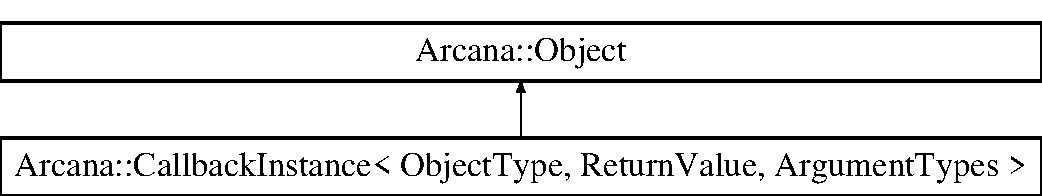
\includegraphics[height=2.000000cm]{class_arcana_1_1_callback_instance}
\end{center}
\end{figure}
\subsection*{Public Member Functions}
\begin{DoxyCompactItemize}
\item 
virtual Return\+Value \mbox{\hyperlink{class_arcana_1_1_callback_instance_aa5bd9b4ee2129a0c22a98f7fa1cfc724}{execute}} (Argument\+Types \&\&... args)=0
\begin{DoxyCompactList}\small\item\em Executes the function. \end{DoxyCompactList}\item 
virtual Return\+Value \mbox{\hyperlink{class_arcana_1_1_callback_instance_af4aced5d787cabb857931ecd87c3ab50}{execute\+If\+Bound}} (Argument\+Types \&\&... args)=0
\begin{DoxyCompactList}\small\item\em Executes the function. \end{DoxyCompactList}\item 
\mbox{\Hypertarget{class_arcana_1_1_callback_instance_a017ab425cf14a399e93cef08d8dbfc71}\label{class_arcana_1_1_callback_instance_a017ab425cf14a399e93cef08d8dbfc71}} 
virtual bool \mbox{\hyperlink{class_arcana_1_1_callback_instance_a017ab425cf14a399e93cef08d8dbfc71}{is\+Bound}} ()=0
\begin{DoxyCompactList}\small\item\em Returns true if a function pointer is bound. \end{DoxyCompactList}\item 
\mbox{\Hypertarget{class_arcana_1_1_callback_instance_a00ff80b8068277052d2814984dfec319}\label{class_arcana_1_1_callback_instance_a00ff80b8068277052d2814984dfec319}} 
virtual bool \mbox{\hyperlink{class_arcana_1_1_callback_instance_a00ff80b8068277052d2814984dfec319}{is\+Static\+Function}} () const =0
\begin{DoxyCompactList}\small\item\em Returns true if a function is a static function. \end{DoxyCompactList}\item 
\mbox{\Hypertarget{class_arcana_1_1_callback_instance_a679d5aba1aa39d3d7609a908b35dd5f3}\label{class_arcana_1_1_callback_instance_a679d5aba1aa39d3d7609a908b35dd5f3}} 
virtual void \mbox{\hyperlink{class_arcana_1_1_callback_instance_a679d5aba1aa39d3d7609a908b35dd5f3}{unbind}} ()=0
\begin{DoxyCompactList}\small\item\em Sets the object and function pointer members to null. \end{DoxyCompactList}\item 
virtual void \mbox{\hyperlink{class_arcana_1_1_callback_instance_a55e87e320e0133a4274c60e87a391a7e}{bind}} (void $\ast$object, void(Object\+::$\ast$)())
\begin{DoxyCompactList}\small\item\em Binds this callback to the member function of an object. \end{DoxyCompactList}\item 
virtual void \mbox{\hyperlink{class_arcana_1_1_callback_instance_a6d9b12af5b8a98b782257a7b10eaa7e9}{bind}} (Return\+Value($\ast$Callback\+Function)(Argument\+Types...))
\begin{DoxyCompactList}\small\item\em Binds a static function pointer to the callback. \end{DoxyCompactList}\end{DoxyCompactItemize}


\subsection{Detailed Description}
\subsubsection*{template$<$typename Object\+Type, typename Return\+Value, typename... Argument\+Types$>$\newline
class Arcana\+::\+Callback\+Instance$<$ Object\+Type, Return\+Value, Argument\+Types $>$}

An instance of a callback. 

This class wraps either a static or member function pointer. Derived classes implement one of the bind methods (one for member functions, one for static functions). 

\subsection{Member Function Documentation}
\mbox{\Hypertarget{class_arcana_1_1_callback_instance_a55e87e320e0133a4274c60e87a391a7e}\label{class_arcana_1_1_callback_instance_a55e87e320e0133a4274c60e87a391a7e}} 
\index{Arcana\+::\+Callback\+Instance@{Arcana\+::\+Callback\+Instance}!bind@{bind}}
\index{bind@{bind}!Arcana\+::\+Callback\+Instance@{Arcana\+::\+Callback\+Instance}}
\subsubsection{\texorpdfstring{bind()}{bind()}\hspace{0.1cm}{\footnotesize\ttfamily [1/2]}}
{\footnotesize\ttfamily template$<$typename Object\+Type, typename Return\+Value, typename... Argument\+Types$>$ \\
virtual void \mbox{\hyperlink{class_arcana_1_1_callback_instance}{Arcana\+::\+Callback\+Instance}}$<$ Object\+Type, Return\+Value, Argument\+Types $>$\+::bind (\begin{DoxyParamCaption}\item[{void $\ast$}]{object,  }\item[{void(Object\+::$\ast$)()}]{ }\end{DoxyParamCaption})\hspace{0.3cm}{\ttfamily [inline]}, {\ttfamily [virtual]}}



Binds this callback to the member function of an object. 

The member function must take the arguments specified in the \mbox{\hyperlink{class_arcana_1_1_callback_instance}{Callback\+Instance}} templates. 

Reimplemented in \mbox{\hyperlink{class_arcana_1_1_member_function_callback_instance_ae93ba2e166f268d480431bb7dfd00140}{Arcana\+::\+Member\+Function\+Callback\+Instance$<$ Object\+Type, Return\+Value, Argument\+Types $>$}}.

\mbox{\Hypertarget{class_arcana_1_1_callback_instance_a6d9b12af5b8a98b782257a7b10eaa7e9}\label{class_arcana_1_1_callback_instance_a6d9b12af5b8a98b782257a7b10eaa7e9}} 
\index{Arcana\+::\+Callback\+Instance@{Arcana\+::\+Callback\+Instance}!bind@{bind}}
\index{bind@{bind}!Arcana\+::\+Callback\+Instance@{Arcana\+::\+Callback\+Instance}}
\subsubsection{\texorpdfstring{bind()}{bind()}\hspace{0.1cm}{\footnotesize\ttfamily [2/2]}}
{\footnotesize\ttfamily template$<$typename Object\+Type, typename Return\+Value, typename... Argument\+Types$>$ \\
virtual void \mbox{\hyperlink{class_arcana_1_1_callback_instance}{Arcana\+::\+Callback\+Instance}}$<$ Object\+Type, Return\+Value, Argument\+Types $>$\+::bind (\begin{DoxyParamCaption}\item[{Return\+Value($\ast$)(Argument\+Types...)}]{Callback\+Function }\end{DoxyParamCaption})\hspace{0.3cm}{\ttfamily [inline]}, {\ttfamily [virtual]}}



Binds a static function pointer to the callback. 

The static function must take the arguments specified in the \mbox{\hyperlink{class_arcana_1_1_callback_instance}{Callback\+Instance}} templates. 

Reimplemented in \mbox{\hyperlink{class_arcana_1_1_static_function_callback_instance_aaf3de60d3146a2cb8946976d73a6ab2c}{Arcana\+::\+Static\+Function\+Callback\+Instance$<$ Return\+Value, Argument\+Types $>$}}.

\mbox{\Hypertarget{class_arcana_1_1_callback_instance_aa5bd9b4ee2129a0c22a98f7fa1cfc724}\label{class_arcana_1_1_callback_instance_aa5bd9b4ee2129a0c22a98f7fa1cfc724}} 
\index{Arcana\+::\+Callback\+Instance@{Arcana\+::\+Callback\+Instance}!execute@{execute}}
\index{execute@{execute}!Arcana\+::\+Callback\+Instance@{Arcana\+::\+Callback\+Instance}}
\subsubsection{\texorpdfstring{execute()}{execute()}}
{\footnotesize\ttfamily template$<$typename Object\+Type, typename Return\+Value, typename... Argument\+Types$>$ \\
virtual Return\+Value \mbox{\hyperlink{class_arcana_1_1_callback_instance}{Arcana\+::\+Callback\+Instance}}$<$ Object\+Type, Return\+Value, Argument\+Types $>$\+::execute (\begin{DoxyParamCaption}\item[{Argument\+Types \&\&...}]{args }\end{DoxyParamCaption})\hspace{0.3cm}{\ttfamily [pure virtual]}}



Executes the function. 

An unknown number of arguments can be passed. The argument types must coincide with the initial arguments specified in the template. 

Implemented in \mbox{\hyperlink{class_arcana_1_1_member_function_callback_instance_aa3da0ee51ae4a6465844c7af67da7d83}{Arcana\+::\+Member\+Function\+Callback\+Instance$<$ Object\+Type, Return\+Value, Argument\+Types $>$}}, and \mbox{\hyperlink{class_arcana_1_1_static_function_callback_instance_a9666f5e80b24e6e38e5d3766a6a577ac}{Arcana\+::\+Static\+Function\+Callback\+Instance$<$ Return\+Value, Argument\+Types $>$}}.

\mbox{\Hypertarget{class_arcana_1_1_callback_instance_af4aced5d787cabb857931ecd87c3ab50}\label{class_arcana_1_1_callback_instance_af4aced5d787cabb857931ecd87c3ab50}} 
\index{Arcana\+::\+Callback\+Instance@{Arcana\+::\+Callback\+Instance}!execute\+If\+Bound@{execute\+If\+Bound}}
\index{execute\+If\+Bound@{execute\+If\+Bound}!Arcana\+::\+Callback\+Instance@{Arcana\+::\+Callback\+Instance}}
\subsubsection{\texorpdfstring{execute\+If\+Bound()}{executeIfBound()}}
{\footnotesize\ttfamily template$<$typename Object\+Type, typename Return\+Value, typename... Argument\+Types$>$ \\
virtual Return\+Value \mbox{\hyperlink{class_arcana_1_1_callback_instance}{Arcana\+::\+Callback\+Instance}}$<$ Object\+Type, Return\+Value, Argument\+Types $>$\+::execute\+If\+Bound (\begin{DoxyParamCaption}\item[{Argument\+Types \&\&...}]{args }\end{DoxyParamCaption})\hspace{0.3cm}{\ttfamily [pure virtual]}}



Executes the function. 

An unknown number of arguments can be passed. The argument types must coincide with the initial arguments specified in the template. This method is the same as \mbox{\hyperlink{class_arcana_1_1_callback_instance_aa5bd9b4ee2129a0c22a98f7fa1cfc724}{execute()}}, but without the assertion. 

Implemented in \mbox{\hyperlink{class_arcana_1_1_member_function_callback_instance_a4d8c12162b9d7b42ad9916d2dba5327d}{Arcana\+::\+Member\+Function\+Callback\+Instance$<$ Object\+Type, Return\+Value, Argument\+Types $>$}}, and \mbox{\hyperlink{class_arcana_1_1_static_function_callback_instance_a1e498222014df725ab8dfb737b48c2ef}{Arcana\+::\+Static\+Function\+Callback\+Instance$<$ Return\+Value, Argument\+Types $>$}}.



The documentation for this class was generated from the following file\+:\begin{DoxyCompactItemize}
\item 
Callback\+Instance.\+h\end{DoxyCompactItemize}

\hypertarget{struct_arcana_1_1_controller_connect_event}{}\section{Arcana\+:\+:Controller\+Connect\+Event Struct Reference}
\label{struct_arcana_1_1_controller_connect_event}\index{Arcana\+::\+Controller\+Connect\+Event@{Arcana\+::\+Controller\+Connect\+Event}}


Controller connection event.  




{\ttfamily \#include $<$Controller\+Connect\+Event.\+h$>$}

Inheritance diagram for Arcana\+:\+:Controller\+Connect\+Event\+:\begin{figure}[H]
\begin{center}
\leavevmode
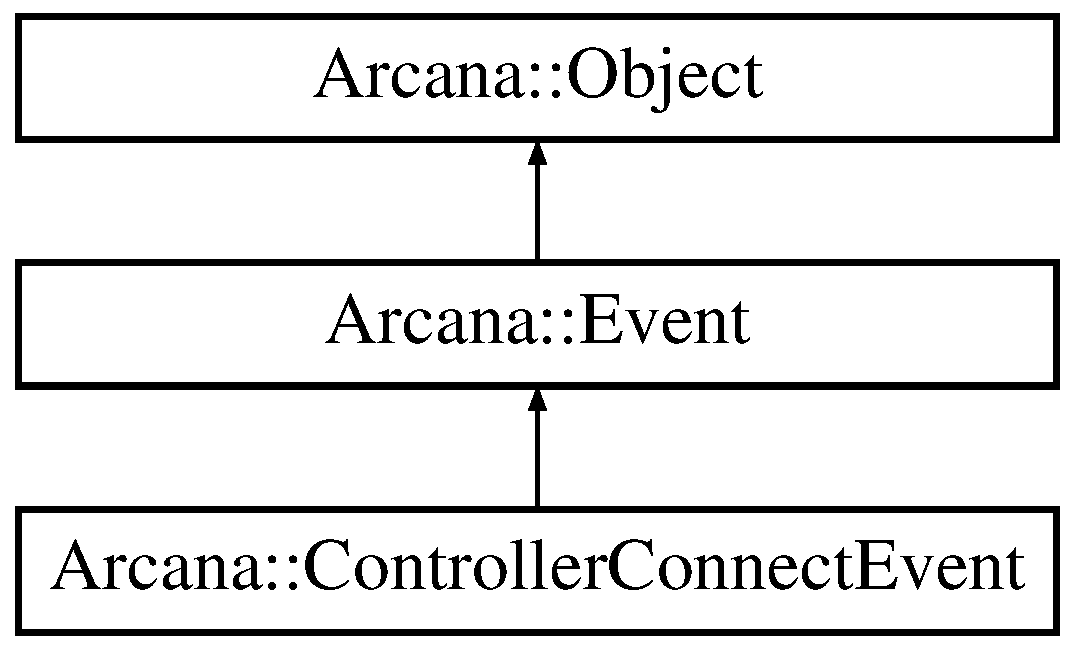
\includegraphics[height=3.000000cm]{struct_arcana_1_1_controller_connect_event}
\end{center}
\end{figure}
\subsection*{Public Types}
\begin{DoxyCompactItemize}
\item 
enum \mbox{\hyperlink{struct_arcana_1_1_controller_connect_event_a13728f4573db87b8b2ef1fc5f9bebc38}{Type}} \{ \mbox{\hyperlink{struct_arcana_1_1_controller_connect_event_a13728f4573db87b8b2ef1fc5f9bebc38a69a33132305627b0998298b76c0f4884}{Connected}}, 
\mbox{\hyperlink{struct_arcana_1_1_controller_connect_event_a13728f4573db87b8b2ef1fc5f9bebc38a067289f89919e46e32ef1a8896c8c2a6}{Disconnected}}
 \}
\begin{DoxyCompactList}\small\item\em Controller event types. \end{DoxyCompactList}\end{DoxyCompactItemize}
\subsection*{Public Member Functions}
\begin{DoxyCompactItemize}
\item 
\mbox{\Hypertarget{struct_arcana_1_1_controller_connect_event_aa55dc359bc98111360e073158ec28a68}\label{struct_arcana_1_1_controller_connect_event_aa55dc359bc98111360e073158ec28a68}} 
\mbox{\hyperlink{struct_arcana_1_1_controller_connect_event_aa55dc359bc98111360e073158ec28a68}{Controller\+Connect\+Event}} (\mbox{\hyperlink{struct_arcana_1_1_controller_connect_event_a13728f4573db87b8b2ef1fc5f9bebc38}{Type}} event, int32 controller\+Id)
\begin{DoxyCompactList}\small\item\em \mbox{\hyperlink{struct_arcana_1_1_controller_connect_event}{Controller\+Connect\+Event}} constructor. \end{DoxyCompactList}\end{DoxyCompactItemize}


\subsection{Detailed Description}
Controller connection event. 

Broadcasted when a new controller is connected/disconnected. Data includes the type (connected or disconnected) and the controller ID. 

\subsection{Member Enumeration Documentation}
\mbox{\Hypertarget{struct_arcana_1_1_controller_connect_event_a13728f4573db87b8b2ef1fc5f9bebc38}\label{struct_arcana_1_1_controller_connect_event_a13728f4573db87b8b2ef1fc5f9bebc38}} 
\index{Arcana\+::\+Controller\+Connect\+Event@{Arcana\+::\+Controller\+Connect\+Event}!Type@{Type}}
\index{Type@{Type}!Arcana\+::\+Controller\+Connect\+Event@{Arcana\+::\+Controller\+Connect\+Event}}
\subsubsection{\texorpdfstring{Type}{Type}}
{\footnotesize\ttfamily enum \mbox{\hyperlink{struct_arcana_1_1_controller_connect_event_a13728f4573db87b8b2ef1fc5f9bebc38}{Arcana\+::\+Controller\+Connect\+Event\+::\+Type}}}



Controller event types. 

\begin{DoxyEnumFields}{Enumerator}
\raisebox{\heightof{T}}[0pt][0pt]{\index{Connected@{Connected}!Arcana\+::\+Controller\+Connect\+Event@{Arcana\+::\+Controller\+Connect\+Event}}\index{Arcana\+::\+Controller\+Connect\+Event@{Arcana\+::\+Controller\+Connect\+Event}!Connected@{Connected}}}\mbox{\Hypertarget{struct_arcana_1_1_controller_connect_event_a13728f4573db87b8b2ef1fc5f9bebc38a69a33132305627b0998298b76c0f4884}\label{struct_arcana_1_1_controller_connect_event_a13728f4573db87b8b2ef1fc5f9bebc38a69a33132305627b0998298b76c0f4884}} 
Connected&Controller connected. \\
\hline

\raisebox{\heightof{T}}[0pt][0pt]{\index{Disconnected@{Disconnected}!Arcana\+::\+Controller\+Connect\+Event@{Arcana\+::\+Controller\+Connect\+Event}}\index{Arcana\+::\+Controller\+Connect\+Event@{Arcana\+::\+Controller\+Connect\+Event}!Disconnected@{Disconnected}}}\mbox{\Hypertarget{struct_arcana_1_1_controller_connect_event_a13728f4573db87b8b2ef1fc5f9bebc38a067289f89919e46e32ef1a8896c8c2a6}\label{struct_arcana_1_1_controller_connect_event_a13728f4573db87b8b2ef1fc5f9bebc38a067289f89919e46e32ef1a8896c8c2a6}} 
Disconnected&Controller disconnected. \\
\hline

\end{DoxyEnumFields}


The documentation for this struct was generated from the following file\+:\begin{DoxyCompactItemize}
\item 
Controller\+Connect\+Event.\+h\end{DoxyCompactItemize}

\hypertarget{class_arcana_1_1_core_module}{}\section{Arcana\+:\+:Core\+Module Class Reference}
\label{class_arcana_1_1_core_module}\index{Arcana\+::\+Core\+Module@{Arcana\+::\+Core\+Module}}


The module interface for the Arcana\+Core module.  




{\ttfamily \#include $<$Core\+Module.\+h$>$}

Inheritance diagram for Arcana\+:\+:Core\+Module\+:\begin{figure}[H]
\begin{center}
\leavevmode
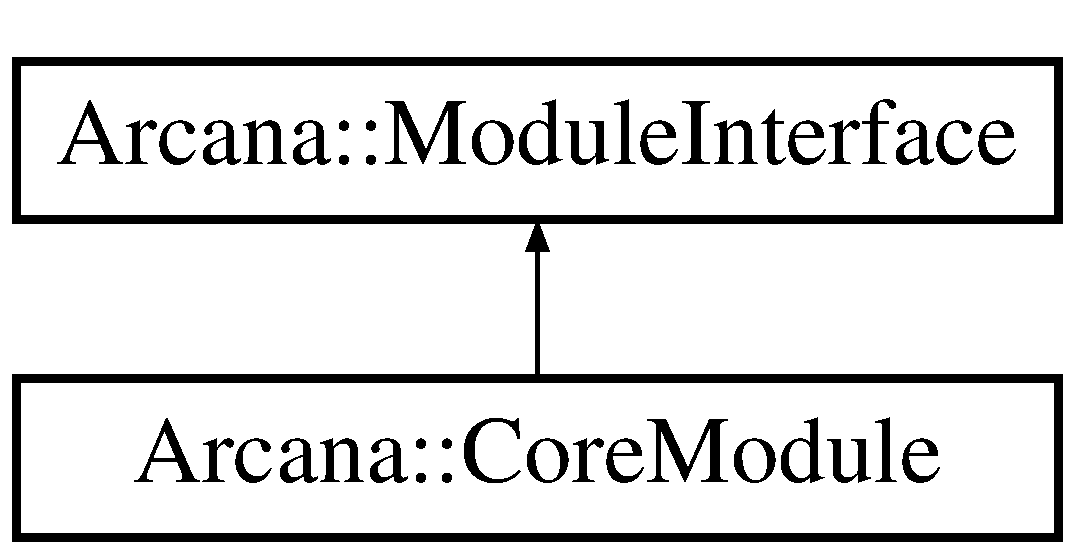
\includegraphics[height=2.000000cm]{class_arcana_1_1_core_module}
\end{center}
\end{figure}
\subsection*{Public Member Functions}
\begin{DoxyCompactItemize}
\item 
\mbox{\Hypertarget{class_arcana_1_1_core_module_a89b8e48937c965b18271089977a085b3}\label{class_arcana_1_1_core_module_a89b8e48937c965b18271089977a085b3}} 
\mbox{\hyperlink{class_arcana_1_1_core_module_a89b8e48937c965b18271089977a085b3}{Core\+Module}} ()
\begin{DoxyCompactList}\small\item\em \mbox{\hyperlink{class_arcana_1_1_core_module}{Core\+Module}} default constructor. \end{DoxyCompactList}\item 
\mbox{\Hypertarget{class_arcana_1_1_core_module_ad4d003080f3890cf3453ce1cd30e2e1c}\label{class_arcana_1_1_core_module_ad4d003080f3890cf3453ce1cd30e2e1c}} 
\mbox{\hyperlink{class_arcana_1_1_core_module_ad4d003080f3890cf3453ce1cd30e2e1c}{$\sim$\+Core\+Module}} ()
\begin{DoxyCompactList}\small\item\em \mbox{\hyperlink{class_arcana_1_1_core_module}{Core\+Module}} destructor. \end{DoxyCompactList}\item 
\mbox{\Hypertarget{class_arcana_1_1_core_module_afe11bce906ee84a565855892a679feed}\label{class_arcana_1_1_core_module_afe11bce906ee84a565855892a679feed}} 
virtual bool \mbox{\hyperlink{class_arcana_1_1_core_module_afe11bce906ee84a565855892a679feed}{start\+Up}} () override
\begin{DoxyCompactList}\small\item\em Starts \mbox{\hyperlink{class_arcana_1_1_core_module}{Core\+Module}} subsystems. \end{DoxyCompactList}\item 
\mbox{\Hypertarget{class_arcana_1_1_core_module_a2d95a9e6a9ce9c985d3de614d71edfff}\label{class_arcana_1_1_core_module_a2d95a9e6a9ce9c985d3de614d71edfff}} 
virtual bool \mbox{\hyperlink{class_arcana_1_1_core_module_a2d95a9e6a9ce9c985d3de614d71edfff}{shut\+Down}} () override
\begin{DoxyCompactList}\small\item\em Shuts down \mbox{\hyperlink{class_arcana_1_1_core_module}{Core\+Module}} subsystems. \end{DoxyCompactList}\item 
virtual bool \mbox{\hyperlink{class_arcana_1_1_core_module_a0b16024de66b0b0f50bac83f20d50c74}{is\+Game\+Module}} () override
\begin{DoxyCompactList}\small\item\em Returns false. \end{DoxyCompactList}\end{DoxyCompactItemize}


\subsection{Detailed Description}
The module interface for the Arcana\+Core module. 

\subsection{Member Function Documentation}
\mbox{\Hypertarget{class_arcana_1_1_core_module_a0b16024de66b0b0f50bac83f20d50c74}\label{class_arcana_1_1_core_module_a0b16024de66b0b0f50bac83f20d50c74}} 
\index{Arcana\+::\+Core\+Module@{Arcana\+::\+Core\+Module}!is\+Game\+Module@{is\+Game\+Module}}
\index{is\+Game\+Module@{is\+Game\+Module}!Arcana\+::\+Core\+Module@{Arcana\+::\+Core\+Module}}
\subsubsection{\texorpdfstring{is\+Game\+Module()}{isGameModule()}}
{\footnotesize\ttfamily bool Arcana\+::\+Core\+Module\+::is\+Game\+Module (\begin{DoxyParamCaption}{ }\end{DoxyParamCaption})\hspace{0.3cm}{\ttfamily [override]}, {\ttfamily [virtual]}}



Returns false. 

The \mbox{\hyperlink{class_arcana_1_1_core_module}{Core\+Module}} is an Arcana\+Engine module. 

Implements \mbox{\hyperlink{class_arcana_1_1_module_interface_a2836a901809149b08e25a36a8e939a44}{Arcana\+::\+Module\+Interface}}.



The documentation for this class was generated from the following files\+:\begin{DoxyCompactItemize}
\item 
Core\+Module.\+h\item 
Core\+Module.\+cpp\end{DoxyCompactItemize}

\hypertarget{class_arcana_1_1_event_1_1_data}{}\section{Arcana\+:\+:Event\+:\+:Data Class Reference}
\label{class_arcana_1_1_event_1_1_data}\index{Arcana\+::\+Event\+::\+Data@{Arcana\+::\+Event\+::\+Data}}


A wrapper for an array of data points.  




{\ttfamily \#include $<$Event.\+h$>$}

\subsection*{Public Member Functions}
\begin{DoxyCompactItemize}
\item 
\mbox{\Hypertarget{class_arcana_1_1_event_1_1_data_a4f6353ff86d50c6cfd1bfc66707497a5}\label{class_arcana_1_1_event_1_1_data_a4f6353ff86d50c6cfd1bfc66707497a5}} 
\mbox{\hyperlink{class_arcana_1_1_event_1_1_data_a4f6353ff86d50c6cfd1bfc66707497a5}{Data}} ()
\begin{DoxyCompactList}\small\item\em \mbox{\hyperlink{class_arcana_1_1_event_1_1_data}{Data}} default constructor. \end{DoxyCompactList}\item 
\mbox{\Hypertarget{class_arcana_1_1_event_1_1_data_a85fb04eff347926ff422bd4101969224}\label{class_arcana_1_1_event_1_1_data_a85fb04eff347926ff422bd4101969224}} 
\mbox{\hyperlink{class_arcana_1_1_event_1_1_data_a85fb04eff347926ff422bd4101969224}{Data}} (const \mbox{\hyperlink{class_arcana_1_1_event_1_1_data}{Data}} \&data)
\begin{DoxyCompactList}\small\item\em \mbox{\hyperlink{class_arcana_1_1_event_1_1_data}{Data}} copy constructor. \end{DoxyCompactList}\item 
\mbox{\hyperlink{class_arcana_1_1_event_1_1_data_a8076fa1e15aa67b9df4c8970bb92d2b9}{$\sim$\+Data}} ()
\begin{DoxyCompactList}\small\item\em \mbox{\hyperlink{class_arcana_1_1_event_1_1_data}{Data}} copy constructor with move. \end{DoxyCompactList}\item 
\mbox{\Hypertarget{class_arcana_1_1_event_1_1_data_a5ad2885d6ad41e64b51e6729331be939}\label{class_arcana_1_1_event_1_1_data_a5ad2885d6ad41e64b51e6729331be939}} 
void \mbox{\hyperlink{class_arcana_1_1_event_1_1_data_a5ad2885d6ad41e64b51e6729331be939}{add\+Double}} (std\+::string name, double entry)
\begin{DoxyCompactList}\small\item\em Adds a data point to the array with a double value. \end{DoxyCompactList}\item 
\mbox{\Hypertarget{class_arcana_1_1_event_1_1_data_ac1cdbf3af77054c8931b0f0b1f9bb354}\label{class_arcana_1_1_event_1_1_data_ac1cdbf3af77054c8931b0f0b1f9bb354}} 
void \mbox{\hyperlink{class_arcana_1_1_event_1_1_data_ac1cdbf3af77054c8931b0f0b1f9bb354}{add\+Float}} (std\+::string name, float entry)
\begin{DoxyCompactList}\small\item\em Adds a data point to the array with a float value. \end{DoxyCompactList}\item 
\mbox{\Hypertarget{class_arcana_1_1_event_1_1_data_a55450bb60c419221c5c5649331ef0bc8}\label{class_arcana_1_1_event_1_1_data_a55450bb60c419221c5c5649331ef0bc8}} 
void \mbox{\hyperlink{class_arcana_1_1_event_1_1_data_a55450bb60c419221c5c5649331ef0bc8}{add\+Int}} (std\+::string name, int entry)
\begin{DoxyCompactList}\small\item\em Adds a data point to the array with an integer value. \end{DoxyCompactList}\item 
\mbox{\Hypertarget{class_arcana_1_1_event_1_1_data_aad93720f1ef41b1ac7e561a497c9205c}\label{class_arcana_1_1_event_1_1_data_aad93720f1ef41b1ac7e561a497c9205c}} 
void \mbox{\hyperlink{class_arcana_1_1_event_1_1_data_aad93720f1ef41b1ac7e561a497c9205c}{add\+Bool}} (std\+::string name, bool entry)
\begin{DoxyCompactList}\small\item\em Adds a data point to the array with a boolean value. \end{DoxyCompactList}\item 
\mbox{\hyperlink{struct_arcana_1_1_event_1_1_data_point}{Data\+Point}} \& \mbox{\hyperlink{class_arcana_1_1_event_1_1_data_ad9fd4aac39a9741d92bb5723b973d3e1}{operator\mbox{[}$\,$\mbox{]}}} (std\+::string name)
\begin{DoxyCompactList}\small\item\em \mbox{\hyperlink{struct_arcana_1_1_event_1_1_data_point}{Data\+Point}} bracket operator. \end{DoxyCompactList}\item 
\mbox{\Hypertarget{class_arcana_1_1_event_1_1_data_ab1477f0496f6c5c3b66f8f1a67380b15}\label{class_arcana_1_1_event_1_1_data_ab1477f0496f6c5c3b66f8f1a67380b15}} 
\mbox{\hyperlink{class_arcana_1_1_event_1_1_data}{Data}} \& \mbox{\hyperlink{class_arcana_1_1_event_1_1_data_ab1477f0496f6c5c3b66f8f1a67380b15}{operator=}} (const \mbox{\hyperlink{class_arcana_1_1_event_1_1_data}{Data}} \&other)
\begin{DoxyCompactList}\small\item\em \mbox{\hyperlink{class_arcana_1_1_event_1_1_data}{Data}} assignment operator. \end{DoxyCompactList}\item 
\mbox{\Hypertarget{class_arcana_1_1_event_1_1_data_a9158bd2be50e69e12c804b880c8acedb}\label{class_arcana_1_1_event_1_1_data_a9158bd2be50e69e12c804b880c8acedb}} 
\mbox{\hyperlink{class_arcana_1_1_event_1_1_data}{Data}} \& \mbox{\hyperlink{class_arcana_1_1_event_1_1_data_a9158bd2be50e69e12c804b880c8acedb}{operator=}} (\mbox{\hyperlink{class_arcana_1_1_event_1_1_data}{Data}} \&\&other)
\begin{DoxyCompactList}\small\item\em \mbox{\hyperlink{class_arcana_1_1_event_1_1_data}{Data}} assignment operator with move. \end{DoxyCompactList}\end{DoxyCompactItemize}


\subsection{Detailed Description}
A wrapper for an array of data points. 

\subsection{Constructor \& Destructor Documentation}
\mbox{\Hypertarget{class_arcana_1_1_event_1_1_data_a8076fa1e15aa67b9df4c8970bb92d2b9}\label{class_arcana_1_1_event_1_1_data_a8076fa1e15aa67b9df4c8970bb92d2b9}} 
\index{Arcana\+::\+Event\+::\+Data@{Arcana\+::\+Event\+::\+Data}!````~Data@{$\sim$\+Data}}
\index{````~Data@{$\sim$\+Data}!Arcana\+::\+Event\+::\+Data@{Arcana\+::\+Event\+::\+Data}}
\subsubsection{\texorpdfstring{$\sim$\+Data()}{~Data()}}
{\footnotesize\ttfamily Arcana\+::\+Event\+::\+Data\+::$\sim$\+Data (\begin{DoxyParamCaption}{ }\end{DoxyParamCaption})}



\mbox{\hyperlink{class_arcana_1_1_event_1_1_data}{Data}} copy constructor with move. 

\mbox{\hyperlink{class_arcana_1_1_event_1_1_data}{Data}} destructor. 

\subsection{Member Function Documentation}
\mbox{\Hypertarget{class_arcana_1_1_event_1_1_data_ad9fd4aac39a9741d92bb5723b973d3e1}\label{class_arcana_1_1_event_1_1_data_ad9fd4aac39a9741d92bb5723b973d3e1}} 
\index{Arcana\+::\+Event\+::\+Data@{Arcana\+::\+Event\+::\+Data}!operator\mbox{[}\mbox{]}@{operator[]}}
\index{operator\mbox{[}\mbox{]}@{operator[]}!Arcana\+::\+Event\+::\+Data@{Arcana\+::\+Event\+::\+Data}}
\subsubsection{\texorpdfstring{operator[]()}{operator[]()}}
{\footnotesize\ttfamily \mbox{\hyperlink{struct_arcana_1_1_event_1_1_data_point}{Event\+::\+Data\+Point}} \& Arcana\+::\+Event\+::\+Data\+::operator\mbox{[}$\,$\mbox{]} (\begin{DoxyParamCaption}\item[{std\+::string}]{name }\end{DoxyParamCaption})}



\mbox{\hyperlink{struct_arcana_1_1_event_1_1_data_point}{Data\+Point}} bracket operator. 

Returns the data point associated with the provided string. 

The documentation for this class was generated from the following files\+:\begin{DoxyCompactItemize}
\item 
Event.\+h\item 
Event.\+cpp\end{DoxyCompactItemize}

\hypertarget{struct_arcana_1_1_event_1_1_data_point}{}\section{Arcana\+:\+:Event\+:\+:Data\+Point Struct Reference}
\label{struct_arcana_1_1_event_1_1_data_point}\index{Arcana\+::\+Event\+::\+Data\+Point@{Arcana\+::\+Event\+::\+Data\+Point}}


A struct that contains a name string and associated data.  




{\ttfamily \#include $<$Event.\+h$>$}

\subsection*{Public Attributes}
\begin{DoxyCompactItemize}
\item 
\mbox{\Hypertarget{struct_arcana_1_1_event_1_1_data_point_a783d241a0db80064fd902076c77509ce}\label{struct_arcana_1_1_event_1_1_data_point_a783d241a0db80064fd902076c77509ce}} 
std\+::string \mbox{\hyperlink{struct_arcana_1_1_event_1_1_data_point_a783d241a0db80064fd902076c77509ce}{\+\_\+name}}
\begin{DoxyCompactList}\small\item\em The name of the data point. \end{DoxyCompactList}\item 
\mbox{\Hypertarget{struct_arcana_1_1_event_1_1_data_point_a97ef64ae8e20b4b884a540eadf8f53e2}\label{struct_arcana_1_1_event_1_1_data_point_a97ef64ae8e20b4b884a540eadf8f53e2}} 
\begin{tabbing}
xx\=xx\=xx\=xx\=xx\=xx\=xx\=xx\=xx\=\kill
union \{\\
\>double \mbox{\hyperlink{struct_arcana_1_1_event_1_1_data_point_a74be14f799c2adeffa2439e959141ca5}{\_double}}\\
\>\>{\em A double value. }\\
\>float \mbox{\hyperlink{struct_arcana_1_1_event_1_1_data_point_afeec2accb12d5842aa9b3ef2a0fbb5ca}{\_float}}\\
\>\>{\em A float value. }\\
\>int \mbox{\hyperlink{struct_arcana_1_1_event_1_1_data_point_ab58be27deb105b240277a102e25dbc8d}{\_int}}\\
\>\>{\em An integer value. }\\
\>bool \mbox{\hyperlink{struct_arcana_1_1_event_1_1_data_point_a4c97bbd1d8eae9c99b36e24fc5004ac6}{\_bool}}\\
\>\>{\em A boolean value. }\\
\}; \\

\end{tabbing}\end{DoxyCompactItemize}


\subsection{Detailed Description}
A struct that contains a name string and associated data. 

The documentation for this struct was generated from the following file\+:\begin{DoxyCompactItemize}
\item 
Event.\+h\end{DoxyCompactItemize}

\hypertarget{class_arcana_1_1_enable_if}{}\section{Arcana\+:\+:Enable\+If$<$ Predicate, Result $>$ Class Template Reference}
\label{class_arcana_1_1_enable_if}\index{Arcana\+::\+Enable\+If$<$ Predicate, Result $>$@{Arcana\+::\+Enable\+If$<$ Predicate, Result $>$}}


The documentation for this class was generated from the following file\+:\begin{DoxyCompactItemize}
\item 
Arcana\+Template.\+h\end{DoxyCompactItemize}

\hypertarget{class_arcana_1_1_enable_if_3_01false_00_01_result_01_4}{}\section{Arcana\+:\+:Enable\+If$<$ false, Result $>$ Class Template Reference}
\label{class_arcana_1_1_enable_if_3_01false_00_01_result_01_4}\index{Arcana\+::\+Enable\+If$<$ false, Result $>$@{Arcana\+::\+Enable\+If$<$ false, Result $>$}}


The documentation for this class was generated from the following file\+:\begin{DoxyCompactItemize}
\item 
Arcana\+Template.\+h\end{DoxyCompactItemize}

\hypertarget{class_arcana_1_1_enable_if_3_01true_00_01_result_01_4}{}\section{Arcana\+:\+:Enable\+If$<$ true, Result $>$ Class Template Reference}
\label{class_arcana_1_1_enable_if_3_01true_00_01_result_01_4}\index{Arcana\+::\+Enable\+If$<$ true, Result $>$@{Arcana\+::\+Enable\+If$<$ true, Result $>$}}
\subsection*{Public Types}
\begin{DoxyCompactItemize}
\item 
\mbox{\Hypertarget{class_arcana_1_1_enable_if_3_01true_00_01_result_01_4_abbf31073a38625a38a1a6341fcc4798c}\label{class_arcana_1_1_enable_if_3_01true_00_01_result_01_4_abbf31073a38625a38a1a6341fcc4798c}} 
typedef Result {\bfseries Type}
\end{DoxyCompactItemize}


The documentation for this class was generated from the following file\+:\begin{DoxyCompactItemize}
\item 
Arcana\+Template.\+h\end{DoxyCompactItemize}

\hypertarget{class_arcana_1_1_event}{}\section{Arcana\+:\+:Event Class Reference}
\label{class_arcana_1_1_event}\index{Arcana\+::\+Event@{Arcana\+::\+Event}}


\mbox{\hyperlink{class_arcana_1_1_event}{Event}} callback typedef.  




{\ttfamily \#include $<$Event.\+h$>$}

Inheritance diagram for Arcana\+:\+:Event\+:\begin{figure}[H]
\begin{center}
\leavevmode
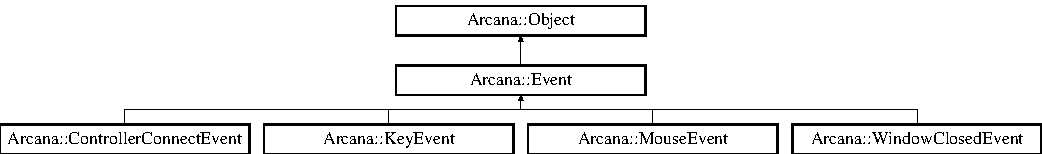
\includegraphics[height=2.068965cm]{class_arcana_1_1_event}
\end{center}
\end{figure}
\subsection*{Classes}
\begin{DoxyCompactItemize}
\item 
class \mbox{\hyperlink{class_arcana_1_1_event_1_1_data}{Data}}
\begin{DoxyCompactList}\small\item\em A wrapper for an array of data points. \end{DoxyCompactList}\item 
struct \mbox{\hyperlink{struct_arcana_1_1_event_1_1_data_point}{Data\+Point}}
\begin{DoxyCompactList}\small\item\em A struct that contains a name string and associated data. \end{DoxyCompactList}\end{DoxyCompactItemize}
\subsection*{Public Member Functions}
\begin{DoxyCompactItemize}
\item 
\mbox{\Hypertarget{class_arcana_1_1_event_a6cf29ea6c699c8841a3bfa8bf64f5623}\label{class_arcana_1_1_event_a6cf29ea6c699c8841a3bfa8bf64f5623}} 
\mbox{\hyperlink{class_arcana_1_1_event_a6cf29ea6c699c8841a3bfa8bf64f5623}{Event}} ()
\begin{DoxyCompactList}\small\item\em \mbox{\hyperlink{class_arcana_1_1_event}{Event}} default constructor. \end{DoxyCompactList}\item 
\mbox{\Hypertarget{class_arcana_1_1_event_acb2a15004697399377c3a7c89fe53814}\label{class_arcana_1_1_event_acb2a15004697399377c3a7c89fe53814}} 
\mbox{\hyperlink{class_arcana_1_1_event_acb2a15004697399377c3a7c89fe53814}{Event}} (uint64 id)
\begin{DoxyCompactList}\small\item\em \mbox{\hyperlink{class_arcana_1_1_event}{Event}} constructor taking the event id as an argument. \end{DoxyCompactList}\item 
\mbox{\Hypertarget{class_arcana_1_1_event_a41b7ce459a149b541efce98358162899}\label{class_arcana_1_1_event_a41b7ce459a149b541efce98358162899}} 
\mbox{\hyperlink{class_arcana_1_1_event_a41b7ce459a149b541efce98358162899}{Event}} (const \mbox{\hyperlink{class_arcana_1_1_event}{Event}} \&event)
\begin{DoxyCompactList}\small\item\em \mbox{\hyperlink{class_arcana_1_1_event}{Event}} copy constructor. \end{DoxyCompactList}\item 
virtual \mbox{\hyperlink{class_arcana_1_1_event_a5e1da20e67addbcecc0d21032573002e}{$\sim$\+Event}} ()
\begin{DoxyCompactList}\small\item\em \mbox{\hyperlink{class_arcana_1_1_event}{Event}} copy constructor with move. \end{DoxyCompactList}\item 
\mbox{\Hypertarget{class_arcana_1_1_event_acdd6f2230b6ac5906a7ae9313b272231}\label{class_arcana_1_1_event_acdd6f2230b6ac5906a7ae9313b272231}} 
uint64 \mbox{\hyperlink{class_arcana_1_1_event_acdd6f2230b6ac5906a7ae9313b272231}{get\+Event\+Id}} () const
\begin{DoxyCompactList}\small\item\em Accessor for the event id. \end{DoxyCompactList}\item 
\mbox{\Hypertarget{class_arcana_1_1_event_a156db327591193d9f949a2079bbc27be}\label{class_arcana_1_1_event_a156db327591193d9f949a2079bbc27be}} 
virtual \mbox{\hyperlink{class_arcana_1_1_event_1_1_data}{Data}} \& \mbox{\hyperlink{class_arcana_1_1_event_a156db327591193d9f949a2079bbc27be}{get\+Data}} ()
\begin{DoxyCompactList}\small\item\em Returns a reference to the event\textquotesingle{}s data. \end{DoxyCompactList}\item 
\mbox{\Hypertarget{class_arcana_1_1_event_aa29eb75e212830a21e0d5956032de557}\label{class_arcana_1_1_event_aa29eb75e212830a21e0d5956032de557}} 
Event\+Callback \& \mbox{\hyperlink{class_arcana_1_1_event_aa29eb75e212830a21e0d5956032de557}{get\+Event\+Callback}} ()
\begin{DoxyCompactList}\small\item\em Accessor for the event\textquotesingle{}s callback. \end{DoxyCompactList}\item 
\mbox{\Hypertarget{class_arcana_1_1_event_a4523da5756dcad3a12ad6877f346280d}\label{class_arcana_1_1_event_a4523da5756dcad3a12ad6877f346280d}} 
double \mbox{\hyperlink{class_arcana_1_1_event_a4523da5756dcad3a12ad6877f346280d}{get\+Double}} (const std\+::string \&name)
\begin{DoxyCompactList}\small\item\em Gets an event data value as a double. \end{DoxyCompactList}\item 
\mbox{\Hypertarget{class_arcana_1_1_event_a5cda5e337cd3d1b934b876e89b6a16ef}\label{class_arcana_1_1_event_a5cda5e337cd3d1b934b876e89b6a16ef}} 
float \mbox{\hyperlink{class_arcana_1_1_event_a5cda5e337cd3d1b934b876e89b6a16ef}{get\+Float}} (const std\+::string \&name)
\begin{DoxyCompactList}\small\item\em Gets an event data value as a float. \end{DoxyCompactList}\item 
\mbox{\Hypertarget{class_arcana_1_1_event_a219085d17da44b6b1eec7d989acac482}\label{class_arcana_1_1_event_a219085d17da44b6b1eec7d989acac482}} 
int \mbox{\hyperlink{class_arcana_1_1_event_a219085d17da44b6b1eec7d989acac482}{get\+Int}} (const std\+::string \&name)
\begin{DoxyCompactList}\small\item\em Gets an event data value as a integer. \end{DoxyCompactList}\item 
\mbox{\Hypertarget{class_arcana_1_1_event_a7f32306719cdc73d3e2a8f4751bc6bb6}\label{class_arcana_1_1_event_a7f32306719cdc73d3e2a8f4751bc6bb6}} 
bool \mbox{\hyperlink{class_arcana_1_1_event_a7f32306719cdc73d3e2a8f4751bc6bb6}{get\+Bool}} (const std\+::string \&name)
\begin{DoxyCompactList}\small\item\em Gets an event data value as a boolean. \end{DoxyCompactList}\item 
\mbox{\Hypertarget{class_arcana_1_1_event_ab1238d3e13e2ce43528ab2dff03affb4}\label{class_arcana_1_1_event_ab1238d3e13e2ce43528ab2dff03affb4}} 
bool \mbox{\hyperlink{class_arcana_1_1_event_ab1238d3e13e2ce43528ab2dff03affb4}{operator==}} (const \mbox{\hyperlink{class_arcana_1_1_event}{Event}} \&other)
\begin{DoxyCompactList}\small\item\em Relational equivalence operator. \end{DoxyCompactList}\item 
\mbox{\Hypertarget{class_arcana_1_1_event_a7ac3cf135728b6c3349f815590093758}\label{class_arcana_1_1_event_a7ac3cf135728b6c3349f815590093758}} 
bool \mbox{\hyperlink{class_arcana_1_1_event_a7ac3cf135728b6c3349f815590093758}{operator==}} (uint64 id)
\begin{DoxyCompactList}\small\item\em Relational equivalence operator, comparing the event id. \end{DoxyCompactList}\item 
\mbox{\Hypertarget{class_arcana_1_1_event_a22b10bbc262a405ea92f06efdff9ab37}\label{class_arcana_1_1_event_a22b10bbc262a405ea92f06efdff9ab37}} 
bool \mbox{\hyperlink{class_arcana_1_1_event_a22b10bbc262a405ea92f06efdff9ab37}{operator!=}} (const \mbox{\hyperlink{class_arcana_1_1_event}{Event}} \&other)
\begin{DoxyCompactList}\small\item\em Relational \textquotesingle{}is not equal to\textquotesingle{} operator. \end{DoxyCompactList}\item 
\mbox{\Hypertarget{class_arcana_1_1_event_abf8a0f5fdd48d07fe85c47b57bd935ce}\label{class_arcana_1_1_event_abf8a0f5fdd48d07fe85c47b57bd935ce}} 
\mbox{\hyperlink{class_arcana_1_1_event}{Event}} \& \mbox{\hyperlink{class_arcana_1_1_event_abf8a0f5fdd48d07fe85c47b57bd935ce}{operator=}} (const \mbox{\hyperlink{class_arcana_1_1_event}{Event}} \&other)
\begin{DoxyCompactList}\small\item\em \mbox{\hyperlink{class_arcana_1_1_event}{Event}} assignment operator. \end{DoxyCompactList}\end{DoxyCompactItemize}


\subsection{Detailed Description}
\mbox{\hyperlink{class_arcana_1_1_event}{Event}} callback typedef. 

If a function is bound by the event, it is called when the event is handled by the Event\+Handler.\+Base class for all event types. 

\subsection{Constructor \& Destructor Documentation}
\mbox{\Hypertarget{class_arcana_1_1_event_a5e1da20e67addbcecc0d21032573002e}\label{class_arcana_1_1_event_a5e1da20e67addbcecc0d21032573002e}} 
\index{Arcana\+::\+Event@{Arcana\+::\+Event}!````~Event@{$\sim$\+Event}}
\index{````~Event@{$\sim$\+Event}!Arcana\+::\+Event@{Arcana\+::\+Event}}
\subsubsection{\texorpdfstring{$\sim$\+Event()}{~Event()}}
{\footnotesize\ttfamily Arcana\+::\+Event\+::$\sim$\+Event (\begin{DoxyParamCaption}{ }\end{DoxyParamCaption})\hspace{0.3cm}{\ttfamily [virtual]}}



\mbox{\hyperlink{class_arcana_1_1_event}{Event}} copy constructor with move. 

\mbox{\hyperlink{class_arcana_1_1_event}{Event}} virtual destructor. 

The documentation for this class was generated from the following files\+:\begin{DoxyCompactItemize}
\item 
Event.\+h\item 
Event.\+cpp\end{DoxyCompactItemize}

\hypertarget{struct_arcana_1_1_timeline_1_1_event_entry}{}\section{Arcana\+:\+:Timeline\+:\+:Event\+Entry Struct Reference}
\label{struct_arcana_1_1_timeline_1_1_event_entry}\index{Arcana\+::\+Timeline\+::\+Event\+Entry@{Arcana\+::\+Timeline\+::\+Event\+Entry}}


An event entry.  




{\ttfamily \#include $<$Timeline.\+h$>$}

\subsection*{Public Attributes}
\begin{DoxyCompactItemize}
\item 
\mbox{\Hypertarget{struct_arcana_1_1_timeline_1_1_event_entry_ac7ab2ec2e47ffc38027df2e5dde49a49}\label{struct_arcana_1_1_timeline_1_1_event_entry_ac7ab2ec2e47ffc38027df2e5dde49a49}} 
\mbox{\hyperlink{class_arcana_1_1_event}{Event}} \mbox{\hyperlink{struct_arcana_1_1_timeline_1_1_event_entry_ac7ab2ec2e47ffc38027df2e5dde49a49}{event}}
\begin{DoxyCompactList}\small\item\em The event to be broadcasted. \end{DoxyCompactList}\item 
\mbox{\Hypertarget{struct_arcana_1_1_timeline_1_1_event_entry_af46b4681e90bd97293fc5f68eb514136}\label{struct_arcana_1_1_timeline_1_1_event_entry_af46b4681e90bd97293fc5f68eb514136}} 
double \mbox{\hyperlink{struct_arcana_1_1_timeline_1_1_event_entry_af46b4681e90bd97293fc5f68eb514136}{time}}
\begin{DoxyCompactList}\small\item\em The time to broadcast the event. \end{DoxyCompactList}\end{DoxyCompactItemize}


\subsection{Detailed Description}
An event entry. 

The documentation for this struct was generated from the following file\+:\begin{DoxyCompactItemize}
\item 
Timeline.\+h\end{DoxyCompactItemize}

\hypertarget{class_arcana_1_1_event_handler}{}\section{Arcana\+:\+:Event\+Handler Class Reference}
\label{class_arcana_1_1_event_handler}\index{Arcana\+::\+Event\+Handler@{Arcana\+::\+Event\+Handler}}


Main class for broadcasting events.  




{\ttfamily \#include $<$Event\+Handler.\+h$>$}

Inheritance diagram for Arcana\+:\+:Event\+Handler\+:\begin{figure}[H]
\begin{center}
\leavevmode
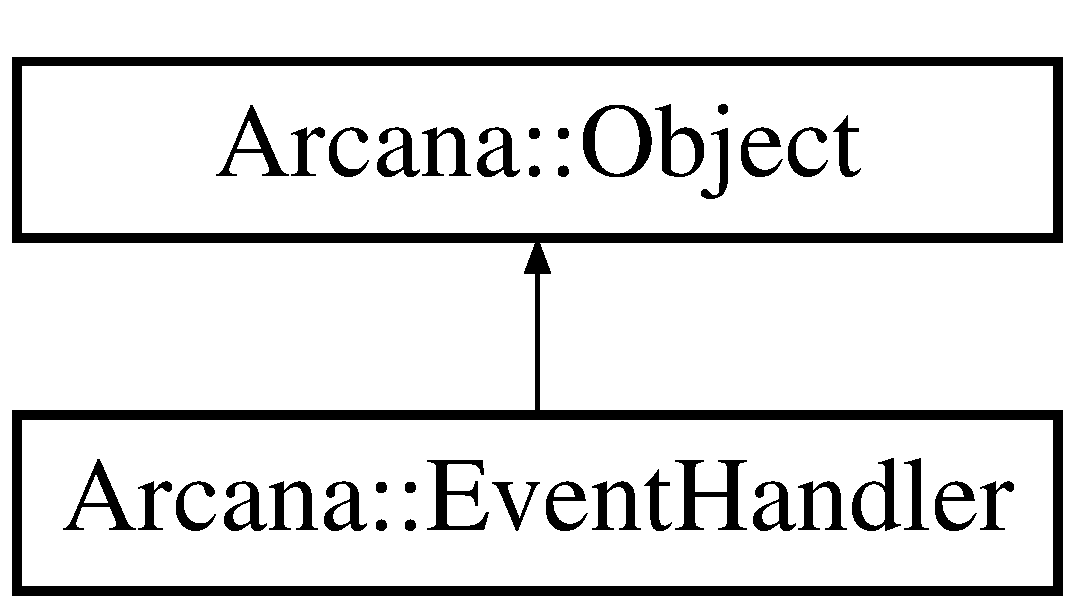
\includegraphics[height=2.000000cm]{class_arcana_1_1_event_handler}
\end{center}
\end{figure}
\subsection*{Classes}
\begin{DoxyCompactItemize}
\item 
class \mbox{\hyperlink{class_arcana_1_1_event_handler_1_1_broadcast_result}{Broadcast\+Result}}
\begin{DoxyCompactList}\small\item\em This class wraps a broadcast result code. It contains methods for easily checking success and getting code strings for debug printing. \end{DoxyCompactList}\end{DoxyCompactItemize}
\subsection*{Public Types}
\begin{DoxyCompactItemize}
\item 
enum \mbox{\hyperlink{class_arcana_1_1_event_handler_a1763837e7c9732fff7df0d4e48b3dbd4}{Broadcast\+Result\+Code}} \+: uint8 \{ \mbox{\hyperlink{class_arcana_1_1_event_handler_a1763837e7c9732fff7df0d4e48b3dbd4a8ea45dcfe2dfc827ecf65d103e18787c}{E\+V\+E\+N\+T\+\_\+\+S\+U\+C\+C\+E\+SS}}, 
\mbox{\hyperlink{class_arcana_1_1_event_handler_a1763837e7c9732fff7df0d4e48b3dbd4a27766aae597f40890345c45fc59dd7f0}{E\+V\+E\+N\+T\+\_\+\+E\+R\+R\+OR}}
 \}
\begin{DoxyCompactList}\small\item\em Enum containing codes for event broadcast success and failure. \end{DoxyCompactList}\item 
\mbox{\Hypertarget{class_arcana_1_1_event_handler_a30e989dae18b9ac3c0bc01aedaea003e}\label{class_arcana_1_1_event_handler_a30e989dae18b9ac3c0bc01aedaea003e}} 
typedef \mbox{\hyperlink{class_arcana_1_1_array}{Array}}$<$ std\+::shared\+\_\+ptr$<$ \mbox{\hyperlink{class_arcana_1_1_event_listener}{Event\+Listener}} $>$ $>$ \mbox{\hyperlink{class_arcana_1_1_event_handler_a30e989dae18b9ac3c0bc01aedaea003e}{Listener\+Array}}
\begin{DoxyCompactList}\small\item\em Typedef for an array of event listeners. \end{DoxyCompactList}\end{DoxyCompactItemize}
\subsection*{Public Member Functions}
\begin{DoxyCompactItemize}
\item 
\mbox{\Hypertarget{class_arcana_1_1_event_handler_abad62db95c13588434b896f7ca556049}\label{class_arcana_1_1_event_handler_abad62db95c13588434b896f7ca556049}} 
\mbox{\hyperlink{class_arcana_1_1_event_handler_abad62db95c13588434b896f7ca556049}{Event\+Handler}} ()
\begin{DoxyCompactList}\small\item\em \mbox{\hyperlink{class_arcana_1_1_event_handler}{Event\+Handler}} default constructor. \end{DoxyCompactList}\item 
\mbox{\Hypertarget{class_arcana_1_1_event_handler_aac9a6d2645d3a74b3b46a10381436c84}\label{class_arcana_1_1_event_handler_aac9a6d2645d3a74b3b46a10381436c84}} 
\mbox{\hyperlink{class_arcana_1_1_event_handler_aac9a6d2645d3a74b3b46a10381436c84}{$\sim$\+Event\+Handler}} ()
\begin{DoxyCompactList}\small\item\em \mbox{\hyperlink{class_arcana_1_1_event_handler}{Event\+Handler}} destructor. \end{DoxyCompactList}\item 
\mbox{\Hypertarget{class_arcana_1_1_event_handler_a1786d06628a98005c406020772adb84a}\label{class_arcana_1_1_event_handler_a1786d06628a98005c406020772adb84a}} 
\mbox{\hyperlink{class_arcana_1_1_event_handler_1_1_broadcast_result}{Broadcast\+Result}} \mbox{\hyperlink{class_arcana_1_1_event_handler_a1786d06628a98005c406020772adb84a}{broadcast}} (\mbox{\hyperlink{class_arcana_1_1_event}{Event}} \&event)
\begin{DoxyCompactList}\small\item\em Broadcasts the event to the event listeners and executes the event callback. \end{DoxyCompactList}\item 
\mbox{\Hypertarget{class_arcana_1_1_event_handler_ae8a53585c131b63aedf362b10c5fbf0f}\label{class_arcana_1_1_event_handler_ae8a53585c131b63aedf362b10c5fbf0f}} 
void \mbox{\hyperlink{class_arcana_1_1_event_handler_ae8a53585c131b63aedf362b10c5fbf0f}{add\+Event\+Listener}} (std\+::shared\+\_\+ptr$<$ \mbox{\hyperlink{class_arcana_1_1_event_listener}{Event\+Listener}} $>$ ptr)
\begin{DoxyCompactList}\small\item\em Adds an event listener to the listener array. \end{DoxyCompactList}\end{DoxyCompactItemize}


\subsection{Detailed Description}
Main class for broadcasting events. 



\subsection{Member Enumeration Documentation}
\mbox{\Hypertarget{class_arcana_1_1_event_handler_a1763837e7c9732fff7df0d4e48b3dbd4}\label{class_arcana_1_1_event_handler_a1763837e7c9732fff7df0d4e48b3dbd4}} 
\index{Arcana\+::\+Event\+Handler@{Arcana\+::\+Event\+Handler}!Broadcast\+Result\+Code@{Broadcast\+Result\+Code}}
\index{Broadcast\+Result\+Code@{Broadcast\+Result\+Code}!Arcana\+::\+Event\+Handler@{Arcana\+::\+Event\+Handler}}
\subsubsection{\texorpdfstring{Broadcast\+Result\+Code}{BroadcastResultCode}}
{\footnotesize\ttfamily enum \mbox{\hyperlink{class_arcana_1_1_event_handler_a1763837e7c9732fff7df0d4e48b3dbd4}{Arcana\+::\+Event\+Handler\+::\+Broadcast\+Result\+Code}} \+: uint8}



Enum containing codes for event broadcast success and failure. 

\begin{DoxyEnumFields}{Enumerator}
\raisebox{\heightof{T}}[0pt][0pt]{\index{E\+V\+E\+N\+T\+\_\+\+S\+U\+C\+C\+E\+SS@{E\+V\+E\+N\+T\+\_\+\+S\+U\+C\+C\+E\+SS}!Arcana\+::\+Event\+Handler@{Arcana\+::\+Event\+Handler}}\index{Arcana\+::\+Event\+Handler@{Arcana\+::\+Event\+Handler}!E\+V\+E\+N\+T\+\_\+\+S\+U\+C\+C\+E\+SS@{E\+V\+E\+N\+T\+\_\+\+S\+U\+C\+C\+E\+SS}}}\mbox{\Hypertarget{class_arcana_1_1_event_handler_a1763837e7c9732fff7df0d4e48b3dbd4a8ea45dcfe2dfc827ecf65d103e18787c}\label{class_arcana_1_1_event_handler_a1763837e7c9732fff7df0d4e48b3dbd4a8ea45dcfe2dfc827ecf65d103e18787c}} 
E\+V\+E\+N\+T\+\_\+\+S\+U\+C\+C\+E\+SS&\mbox{\hyperlink{class_arcana_1_1_event}{Event}} was broadcasted successfully. \\
\hline

\raisebox{\heightof{T}}[0pt][0pt]{\index{E\+V\+E\+N\+T\+\_\+\+E\+R\+R\+OR@{E\+V\+E\+N\+T\+\_\+\+E\+R\+R\+OR}!Arcana\+::\+Event\+Handler@{Arcana\+::\+Event\+Handler}}\index{Arcana\+::\+Event\+Handler@{Arcana\+::\+Event\+Handler}!E\+V\+E\+N\+T\+\_\+\+E\+R\+R\+OR@{E\+V\+E\+N\+T\+\_\+\+E\+R\+R\+OR}}}\mbox{\Hypertarget{class_arcana_1_1_event_handler_a1763837e7c9732fff7df0d4e48b3dbd4a27766aae597f40890345c45fc59dd7f0}\label{class_arcana_1_1_event_handler_a1763837e7c9732fff7df0d4e48b3dbd4a27766aae597f40890345c45fc59dd7f0}} 
E\+V\+E\+N\+T\+\_\+\+E\+R\+R\+OR&\mbox{\hyperlink{class_arcana_1_1_event}{Event}} was broadcasted unsuccessfully. \\
\hline

\end{DoxyEnumFields}


The documentation for this class was generated from the following files\+:\begin{DoxyCompactItemize}
\item 
Event\+Handler.\+h\item 
Event\+Handler.\+cpp\end{DoxyCompactItemize}

\hypertarget{class_arcana_1_1_event_listener}{}\section{Arcana\+:\+:Event\+Listener Class Reference}
\label{class_arcana_1_1_event_listener}\index{Arcana\+::\+Event\+Listener@{Arcana\+::\+Event\+Listener}}


An interface for processing events.  




{\ttfamily \#include $<$Event\+Listener.\+h$>$}

\subsection*{Public Member Functions}
\begin{DoxyCompactItemize}
\item 
\mbox{\Hypertarget{class_arcana_1_1_event_listener_a10c321f4ac5dc480e531318bc7f69cf1}\label{class_arcana_1_1_event_listener_a10c321f4ac5dc480e531318bc7f69cf1}} 
virtual \mbox{\hyperlink{class_arcana_1_1_event_listener_a10c321f4ac5dc480e531318bc7f69cf1}{$\sim$\+Event\+Listener}} ()
\begin{DoxyCompactList}\small\item\em \mbox{\hyperlink{class_arcana_1_1_event_listener}{Event\+Listener}} virtual destructor. \end{DoxyCompactList}\item 
\mbox{\Hypertarget{class_arcana_1_1_event_listener_a48fe1036f39b1bef9fd307c8fed29ad3}\label{class_arcana_1_1_event_listener_a48fe1036f39b1bef9fd307c8fed29ad3}} 
virtual bool \mbox{\hyperlink{class_arcana_1_1_event_listener_a48fe1036f39b1bef9fd307c8fed29ad3}{process\+Event}} (\mbox{\hyperlink{class_arcana_1_1_event}{Event}} \&event, \mbox{\hyperlink{class_arcana_1_1_event_handler}{Event\+Handler}} \&handler)=0
\begin{DoxyCompactList}\small\item\em Pure virtual process event function. This function must be overriden in all derived classes. \end{DoxyCompactList}\item 
\mbox{\Hypertarget{class_arcana_1_1_event_listener_acbbf1255b97403f3f368bbd2929cd55b}\label{class_arcana_1_1_event_listener_acbbf1255b97403f3f368bbd2929cd55b}} 
void \mbox{\hyperlink{class_arcana_1_1_event_listener_acbbf1255b97403f3f368bbd2929cd55b}{listen\+For\+Event}} (uint64 event\+Id)
\begin{DoxyCompactList}\small\item\em Adds an event id to the list of listened events. The event listener will listen for events with the specified id. \end{DoxyCompactList}\item 
\mbox{\Hypertarget{class_arcana_1_1_event_listener_a63e5e68d753941f21711f7b91d123239}\label{class_arcana_1_1_event_listener_a63e5e68d753941f21711f7b91d123239}} 
bool \mbox{\hyperlink{class_arcana_1_1_event_listener_a63e5e68d753941f21711f7b91d123239}{is\+Listening\+For\+Event}} (uint64 event\+Id) const
\begin{DoxyCompactList}\small\item\em Returns true if the listener is listening for events with this id. \end{DoxyCompactList}\end{DoxyCompactItemize}


\subsection{Detailed Description}
An interface for processing events. 

This is the base class for all other classes that need to process events. There are methods for setting specific event ids to listen for. This eliminates the need to check the event id in the process event method. 

The documentation for this class was generated from the following file\+:\begin{DoxyCompactItemize}
\item 
Event\+Listener.\+h\end{DoxyCompactItemize}

\hypertarget{class_arcana_1_1_global_object_i_d}{}\section{Arcana\+:\+:Global\+Object\+ID Class Reference}
\label{class_arcana_1_1_global_object_i_d}\index{Arcana\+::\+Global\+Object\+ID@{Arcana\+::\+Global\+Object\+ID}}


A global object id.  




{\ttfamily \#include $<$Global\+Object\+I\+D.\+h$>$}

\subsection*{Public Member Functions}
\begin{DoxyCompactItemize}
\item 
\mbox{\Hypertarget{class_arcana_1_1_global_object_i_d_aee4024285c58e530085557f363358b36}\label{class_arcana_1_1_global_object_i_d_aee4024285c58e530085557f363358b36}} 
\mbox{\hyperlink{class_arcana_1_1_global_object_i_d_aee4024285c58e530085557f363358b36}{Global\+Object\+ID}} ()
\begin{DoxyCompactList}\small\item\em \mbox{\hyperlink{class_arcana_1_1_global_object_i_d}{Global\+Object\+ID}} default constructor. \end{DoxyCompactList}\item 
\mbox{\Hypertarget{class_arcana_1_1_global_object_i_d_a519bd86deae4034f8b0ca32c17b62870}\label{class_arcana_1_1_global_object_i_d_a519bd86deae4034f8b0ca32c17b62870}} 
\mbox{\hyperlink{class_arcana_1_1_global_object_i_d_a519bd86deae4034f8b0ca32c17b62870}{Global\+Object\+ID}} (const std\+::string \&name)
\begin{DoxyCompactList}\small\item\em \mbox{\hyperlink{class_arcana_1_1_global_object_i_d}{Global\+Object\+ID}} constructor with name argument. \end{DoxyCompactList}\item 
\mbox{\hyperlink{class_arcana_1_1_global_object_i_d_a85279618fe9f94d268db594a2d07ab2a}{Global\+Object\+ID}} (const std\+::string \&name, int64 id)
\begin{DoxyCompactList}\small\item\em \mbox{\hyperlink{class_arcana_1_1_global_object_i_d}{Global\+Object\+ID}} constructor with both name and id arguments. \end{DoxyCompactList}\item 
\mbox{\Hypertarget{class_arcana_1_1_global_object_i_d_a37b662e8d38746d0c7e9b71a25fa5937}\label{class_arcana_1_1_global_object_i_d_a37b662e8d38746d0c7e9b71a25fa5937}} 
\mbox{\hyperlink{class_arcana_1_1_global_object_i_d_a37b662e8d38746d0c7e9b71a25fa5937}{$\sim$\+Global\+Object\+ID}} ()
\begin{DoxyCompactList}\small\item\em \mbox{\hyperlink{class_arcana_1_1_global_object_i_d}{Global\+Object\+ID}} destructor. \end{DoxyCompactList}\item 
\mbox{\Hypertarget{class_arcana_1_1_global_object_i_d_a5cfa274ebc29b062146c502ff465abd5}\label{class_arcana_1_1_global_object_i_d_a5cfa274ebc29b062146c502ff465abd5}} 
int64 \mbox{\hyperlink{class_arcana_1_1_global_object_i_d_a5cfa274ebc29b062146c502ff465abd5}{hash\+String}} (const std\+::string \&string)
\begin{DoxyCompactList}\small\item\em Hashes a string. Converts a string into a 64-\/bit integer. \end{DoxyCompactList}\item 
\mbox{\Hypertarget{class_arcana_1_1_global_object_i_d_a7288b8c074f8e223befa23feefe49f26}\label{class_arcana_1_1_global_object_i_d_a7288b8c074f8e223befa23feefe49f26}} 
const std\+::string \& \mbox{\hyperlink{class_arcana_1_1_global_object_i_d_a7288b8c074f8e223befa23feefe49f26}{get\+Name}} () const
\begin{DoxyCompactList}\small\item\em Accessor for the object\textquotesingle{}s name. \end{DoxyCompactList}\item 
\mbox{\Hypertarget{class_arcana_1_1_global_object_i_d_a045bc497b915b4c5ca87601664f08baf}\label{class_arcana_1_1_global_object_i_d_a045bc497b915b4c5ca87601664f08baf}} 
int64 \mbox{\hyperlink{class_arcana_1_1_global_object_i_d_a045bc497b915b4c5ca87601664f08baf}{get\+Id}} () const
\begin{DoxyCompactList}\small\item\em Accessor for the object\textquotesingle{}s integer id. \end{DoxyCompactList}\item 
\mbox{\Hypertarget{class_arcana_1_1_global_object_i_d_a9ef5aba9aa2aa290ac8eb57683135f55}\label{class_arcana_1_1_global_object_i_d_a9ef5aba9aa2aa290ac8eb57683135f55}} 
bool \mbox{\hyperlink{class_arcana_1_1_global_object_i_d_a9ef5aba9aa2aa290ac8eb57683135f55}{operator==}} (const \mbox{\hyperlink{class_arcana_1_1_global_object_i_d}{Global\+Object\+ID}} \&other) const
\begin{DoxyCompactList}\small\item\em Relational equivalence operator. Compares the Global\+Object\+I\+Ds\textquotesingle{} integer ids, rather than the names. \end{DoxyCompactList}\end{DoxyCompactItemize}


\subsection{Detailed Description}
A global object id. 

This class takes a name string and hashes it. This allows object ids to be compared using the hashed value, eliminating the need for string comparisons. 

\subsection{Constructor \& Destructor Documentation}
\mbox{\Hypertarget{class_arcana_1_1_global_object_i_d_a85279618fe9f94d268db594a2d07ab2a}\label{class_arcana_1_1_global_object_i_d_a85279618fe9f94d268db594a2d07ab2a}} 
\index{Arcana\+::\+Global\+Object\+ID@{Arcana\+::\+Global\+Object\+ID}!Global\+Object\+ID@{Global\+Object\+ID}}
\index{Global\+Object\+ID@{Global\+Object\+ID}!Arcana\+::\+Global\+Object\+ID@{Arcana\+::\+Global\+Object\+ID}}
\subsubsection{\texorpdfstring{Global\+Object\+I\+D()}{GlobalObjectID()}}
{\footnotesize\ttfamily Arcana\+::\+Global\+Object\+I\+D\+::\+Global\+Object\+ID (\begin{DoxyParamCaption}\item[{const std\+::string \&}]{name,  }\item[{int64}]{id }\end{DoxyParamCaption})}



\mbox{\hyperlink{class_arcana_1_1_global_object_i_d}{Global\+Object\+ID}} constructor with both name and id arguments. 

This constructor can be dangerous if the user creates two Global\+Object\+I\+Ds with the same integer id. Two Global\+Object\+I\+Ds with different names would be equal. 

The documentation for this class was generated from the following files\+:\begin{DoxyCompactItemize}
\item 
Global\+Object\+I\+D.\+h\item 
Global\+Object\+I\+D.\+cpp\end{DoxyCompactItemize}

\hypertarget{class_arcana_1_1_indexed_container_iterator}{}\section{Arcana\+:\+:Indexed\+Container\+Iterator$<$ Container\+Type, Element\+Type, Index\+Type $>$ Class Template Reference}
\label{class_arcana_1_1_indexed_container_iterator}\index{Arcana\+::\+Indexed\+Container\+Iterator$<$ Container\+Type, Element\+Type, Index\+Type $>$@{Arcana\+::\+Indexed\+Container\+Iterator$<$ Container\+Type, Element\+Type, Index\+Type $>$}}


Iterator for custom Arcana\+Engine containers.  




{\ttfamily \#include $<$Array.\+h$>$}

\subsection*{Public Member Functions}
\begin{DoxyCompactItemize}
\item 
\mbox{\Hypertarget{class_arcana_1_1_indexed_container_iterator_a032c1a8170b6ed3cb626c460a56ef579}\label{class_arcana_1_1_indexed_container_iterator_a032c1a8170b6ed3cb626c460a56ef579}} 
\mbox{\hyperlink{class_arcana_1_1_indexed_container_iterator_a032c1a8170b6ed3cb626c460a56ef579}{Indexed\+Container\+Iterator}} (Container\+Type \&container, Index\+Type start\+Index=0)
\begin{DoxyCompactList}\small\item\em \mbox{\hyperlink{class_arcana_1_1_indexed_container_iterator}{Indexed\+Container\+Iterator}} constructor. This constructor takes a reference to the container and the starting index as arguments. Rarely used as containers provide create\+Iterator() methods. Can be used with user-\/created containers. \end{DoxyCompactList}\item 
\mbox{\Hypertarget{class_arcana_1_1_indexed_container_iterator_ae38b4d8cace7e619dd4f0c58bda29931}\label{class_arcana_1_1_indexed_container_iterator_ae38b4d8cace7e619dd4f0c58bda29931}} 
\mbox{\hyperlink{class_arcana_1_1_indexed_container_iterator}{Indexed\+Container\+Iterator}} \& \mbox{\hyperlink{class_arcana_1_1_indexed_container_iterator_ae38b4d8cace7e619dd4f0c58bda29931}{operator++}} ()
\begin{DoxyCompactList}\small\item\em Prefix increment operator. Increments the index of the iterator. \end{DoxyCompactList}\item 
\mbox{\Hypertarget{class_arcana_1_1_indexed_container_iterator_afcae22817d6746ddb9a1d3686627346d}\label{class_arcana_1_1_indexed_container_iterator_afcae22817d6746ddb9a1d3686627346d}} 
\mbox{\hyperlink{class_arcana_1_1_indexed_container_iterator}{Indexed\+Container\+Iterator}} \mbox{\hyperlink{class_arcana_1_1_indexed_container_iterator_afcae22817d6746ddb9a1d3686627346d}{operator++}} (int)
\begin{DoxyCompactList}\small\item\em Postfix increment operator. Increments the index of the iterator. \end{DoxyCompactList}\item 
\mbox{\Hypertarget{class_arcana_1_1_indexed_container_iterator_a5c8c3f653393934e47da75e894ccf0e7}\label{class_arcana_1_1_indexed_container_iterator_a5c8c3f653393934e47da75e894ccf0e7}} 
\mbox{\hyperlink{class_arcana_1_1_indexed_container_iterator}{Indexed\+Container\+Iterator}} \& \mbox{\hyperlink{class_arcana_1_1_indexed_container_iterator_a5c8c3f653393934e47da75e894ccf0e7}{operator-\/-\/}} ()
\begin{DoxyCompactList}\small\item\em Prefix decrement operator. Decrements the index of the iterator. \end{DoxyCompactList}\item 
\mbox{\Hypertarget{class_arcana_1_1_indexed_container_iterator_a2ad604565d2e6e855b0bba4c9f657cdf}\label{class_arcana_1_1_indexed_container_iterator_a2ad604565d2e6e855b0bba4c9f657cdf}} 
\mbox{\hyperlink{class_arcana_1_1_indexed_container_iterator}{Indexed\+Container\+Iterator}} \mbox{\hyperlink{class_arcana_1_1_indexed_container_iterator_a2ad604565d2e6e855b0bba4c9f657cdf}{operator-\/-\/}} (int)
\begin{DoxyCompactList}\small\item\em Postfix decrement operator. Decrements the index of the iterator. \end{DoxyCompactList}\item 
\mbox{\Hypertarget{class_arcana_1_1_indexed_container_iterator_a67ac83c9256b5c09ab56242ef89216ab}\label{class_arcana_1_1_indexed_container_iterator_a67ac83c9256b5c09ab56242ef89216ab}} 
\mbox{\hyperlink{class_arcana_1_1_indexed_container_iterator}{Indexed\+Container\+Iterator}} \& \mbox{\hyperlink{class_arcana_1_1_indexed_container_iterator_a67ac83c9256b5c09ab56242ef89216ab}{operator+=}} (int32 offset)
\begin{DoxyCompactList}\small\item\em Addition assignment operator. Adds an offset to the index of the iterator. \end{DoxyCompactList}\item 
\mbox{\Hypertarget{class_arcana_1_1_indexed_container_iterator_a88855965dd71c21fa2b554d1f15f2485}\label{class_arcana_1_1_indexed_container_iterator_a88855965dd71c21fa2b554d1f15f2485}} 
\mbox{\hyperlink{class_arcana_1_1_indexed_container_iterator}{Indexed\+Container\+Iterator}} \mbox{\hyperlink{class_arcana_1_1_indexed_container_iterator_a88855965dd71c21fa2b554d1f15f2485}{operator+}} (int32 offset) const
\begin{DoxyCompactList}\small\item\em Addition operator. Adds an offset to the index of the iterator. \end{DoxyCompactList}\item 
\mbox{\Hypertarget{class_arcana_1_1_indexed_container_iterator_aee19f0a97e3595af3fd06e33de5dd1a6}\label{class_arcana_1_1_indexed_container_iterator_aee19f0a97e3595af3fd06e33de5dd1a6}} 
\mbox{\hyperlink{class_arcana_1_1_indexed_container_iterator}{Indexed\+Container\+Iterator}} \& \mbox{\hyperlink{class_arcana_1_1_indexed_container_iterator_aee19f0a97e3595af3fd06e33de5dd1a6}{operator-\/=}} (int32 offset)
\begin{DoxyCompactList}\small\item\em Subtraction assignment operator. Subtracts an offset to the index of the iterator. \end{DoxyCompactList}\item 
\mbox{\Hypertarget{class_arcana_1_1_indexed_container_iterator_a4245cbd35b75c07a98da57b7fc534268}\label{class_arcana_1_1_indexed_container_iterator_a4245cbd35b75c07a98da57b7fc534268}} 
\mbox{\hyperlink{class_arcana_1_1_indexed_container_iterator}{Indexed\+Container\+Iterator}} \mbox{\hyperlink{class_arcana_1_1_indexed_container_iterator_a4245cbd35b75c07a98da57b7fc534268}{operator-\/}} (int32 offset) const
\begin{DoxyCompactList}\small\item\em Subtraction operator. Subtracts an offset to the index of the iterator. \end{DoxyCompactList}\item 
\mbox{\Hypertarget{class_arcana_1_1_indexed_container_iterator_aeef395899950a68702ef3c198e93faa3}\label{class_arcana_1_1_indexed_container_iterator_aeef395899950a68702ef3c198e93faa3}} 
Element\+Type \& \mbox{\hyperlink{class_arcana_1_1_indexed_container_iterator_aeef395899950a68702ef3c198e93faa3}{operator$\ast$}} () const
\begin{DoxyCompactList}\small\item\em Dereference operator. Returns a reference to the container element at the current index. \end{DoxyCompactList}\item 
\mbox{\Hypertarget{class_arcana_1_1_indexed_container_iterator_ac389ea0b34f03ca8ada424b31cfc8729}\label{class_arcana_1_1_indexed_container_iterator_ac389ea0b34f03ca8ada424b31cfc8729}} 
Element\+Type $\ast$ \mbox{\hyperlink{class_arcana_1_1_indexed_container_iterator_ac389ea0b34f03ca8ada424b31cfc8729}{operator-\/$>$}} () const
\begin{DoxyCompactList}\small\item\em Overload of pointer member selection operator. Returns a pointer to the container element at the current index. \end{DoxyCompactList}\item 
\mbox{\Hypertarget{class_arcana_1_1_indexed_container_iterator_a1d82d3b238967897232940197d20f9e0}\label{class_arcana_1_1_indexed_container_iterator_a1d82d3b238967897232940197d20f9e0}} 
\mbox{\hyperlink{class_arcana_1_1_indexed_container_iterator_a1d82d3b238967897232940197d20f9e0}{operator bool}} () const
\begin{DoxyCompactList}\small\item\em Boolean conversion operator. Returns true if the current index is valid. Uses \mbox{\hyperlink{class_arcana_1_1_array_a0b1c26013b63c374bc9e980e364d6e14}{Array.\+is\+Valid\+Index()}}. \end{DoxyCompactList}\item 
\mbox{\Hypertarget{class_arcana_1_1_indexed_container_iterator_a2ae1b46ef9ed0bd49688b9537f131db5}\label{class_arcana_1_1_indexed_container_iterator_a2ae1b46ef9ed0bd49688b9537f131db5}} 
bool \mbox{\hyperlink{class_arcana_1_1_indexed_container_iterator_a2ae1b46ef9ed0bd49688b9537f131db5}{operator!}} () const
\begin{DoxyCompactList}\small\item\em Logical negation operator. Returns false if the current index is valid. Uses \mbox{\hyperlink{class_arcana_1_1_array_a0b1c26013b63c374bc9e980e364d6e14}{Array.\+is\+Valid\+Index()}}. \end{DoxyCompactList}\item 
\mbox{\Hypertarget{class_arcana_1_1_indexed_container_iterator_a3b5249b938cb2de4e2006507e798bc3f}\label{class_arcana_1_1_indexed_container_iterator_a3b5249b938cb2de4e2006507e798bc3f}} 
Index\+Type \mbox{\hyperlink{class_arcana_1_1_indexed_container_iterator_a3b5249b938cb2de4e2006507e798bc3f}{get\+Index}} () const
\begin{DoxyCompactList}\small\item\em Returns the current index. \end{DoxyCompactList}\item 
\mbox{\Hypertarget{class_arcana_1_1_indexed_container_iterator_ac7e898263ea6deccf714b8f7ed72e9e9}\label{class_arcana_1_1_indexed_container_iterator_ac7e898263ea6deccf714b8f7ed72e9e9}} 
void \mbox{\hyperlink{class_arcana_1_1_indexed_container_iterator_ac7e898263ea6deccf714b8f7ed72e9e9}{reset}} ()
\begin{DoxyCompactList}\small\item\em Resets the index to zero. \end{DoxyCompactList}\end{DoxyCompactItemize}
\subsection*{Friends}
\begin{DoxyCompactItemize}
\item 
\mbox{\Hypertarget{class_arcana_1_1_indexed_container_iterator_a194105b67fc3a701928282938eea8f91}\label{class_arcana_1_1_indexed_container_iterator_a194105b67fc3a701928282938eea8f91}} 
bool \mbox{\hyperlink{class_arcana_1_1_indexed_container_iterator_a194105b67fc3a701928282938eea8f91}{operator==}} (const \mbox{\hyperlink{class_arcana_1_1_indexed_container_iterator}{Indexed\+Container\+Iterator}} \&lhs, const \mbox{\hyperlink{class_arcana_1_1_indexed_container_iterator}{Indexed\+Container\+Iterator}} \&rhs)
\begin{DoxyCompactList}\small\item\em Relational equivalence operator. Returns true if both the container and index of the two iterators are equal. \end{DoxyCompactList}\item 
\mbox{\Hypertarget{class_arcana_1_1_indexed_container_iterator_a3f8f1d6ae101307b62e1f5709cc10eb4}\label{class_arcana_1_1_indexed_container_iterator_a3f8f1d6ae101307b62e1f5709cc10eb4}} 
bool \mbox{\hyperlink{class_arcana_1_1_indexed_container_iterator_a3f8f1d6ae101307b62e1f5709cc10eb4}{operator!=}} (const \mbox{\hyperlink{class_arcana_1_1_indexed_container_iterator}{Indexed\+Container\+Iterator}} \&lhs, const \mbox{\hyperlink{class_arcana_1_1_indexed_container_iterator}{Indexed\+Container\+Iterator}} \&rhs)
\begin{DoxyCompactList}\small\item\em Relational \char`\"{}is not equal to\char`\"{} operator. Returns false if the container or index of the two iterators are equal. \end{DoxyCompactList}\end{DoxyCompactItemize}


\subsection{Detailed Description}
\subsubsection*{template$<$typename Container\+Type, typename Element\+Type, typename Index\+Type$>$\newline
class Arcana\+::\+Indexed\+Container\+Iterator$<$ Container\+Type, Element\+Type, Index\+Type $>$}

Iterator for custom Arcana\+Engine containers. 

\mbox{\hyperlink{class_arcana_1_1_array}{Array}} iterators are created easily with Array.\+create\+Iterator() or Array.\+create\+Const\+Iterator(). This class provides operators for incrementing or decrementing the array index. Using the dereference operator returns a reference to the array element at the current index. 

The documentation for this class was generated from the following file\+:\begin{DoxyCompactItemize}
\item 
Array.\+h\end{DoxyCompactItemize}

\hypertarget{struct_arcana_1_1_is_base_of}{}\section{Arcana\+:\+:Is\+Base\+Of$<$ A, B $>$ Struct Template Reference}
\label{struct_arcana_1_1_is_base_of}\index{Arcana\+::\+Is\+Base\+Of$<$ A, B $>$@{Arcana\+::\+Is\+Base\+Of$<$ A, B $>$}}
\subsection*{Public Types}
\begin{DoxyCompactItemize}
\item 
\mbox{\Hypertarget{struct_arcana_1_1_is_base_of_a5c686e226da2d0fda99277d9f61121a1}\label{struct_arcana_1_1_is_base_of_a5c686e226da2d0fda99277d9f61121a1}} 
enum \{ {\bfseries Value} = std\+:\+:is\+\_\+base\+\_\+of$<$A, B$>$\+:\+:value
 \}
\end{DoxyCompactItemize}


The documentation for this struct was generated from the following file\+:\begin{DoxyCompactItemize}
\item 
Type\+Traits.\+h\end{DoxyCompactItemize}

\hypertarget{class_arcana_1_1_key_event}{}\section{Arcana\+:\+:Key\+Event Class Reference}
\label{class_arcana_1_1_key_event}\index{Arcana\+::\+Key\+Event@{Arcana\+::\+Key\+Event}}


\mbox{\hyperlink{class_arcana_1_1_event}{Event}} broadcasted on key presses/releases.  




{\ttfamily \#include $<$Key\+Event.\+h$>$}

Inheritance diagram for Arcana\+:\+:Key\+Event\+:\begin{figure}[H]
\begin{center}
\leavevmode
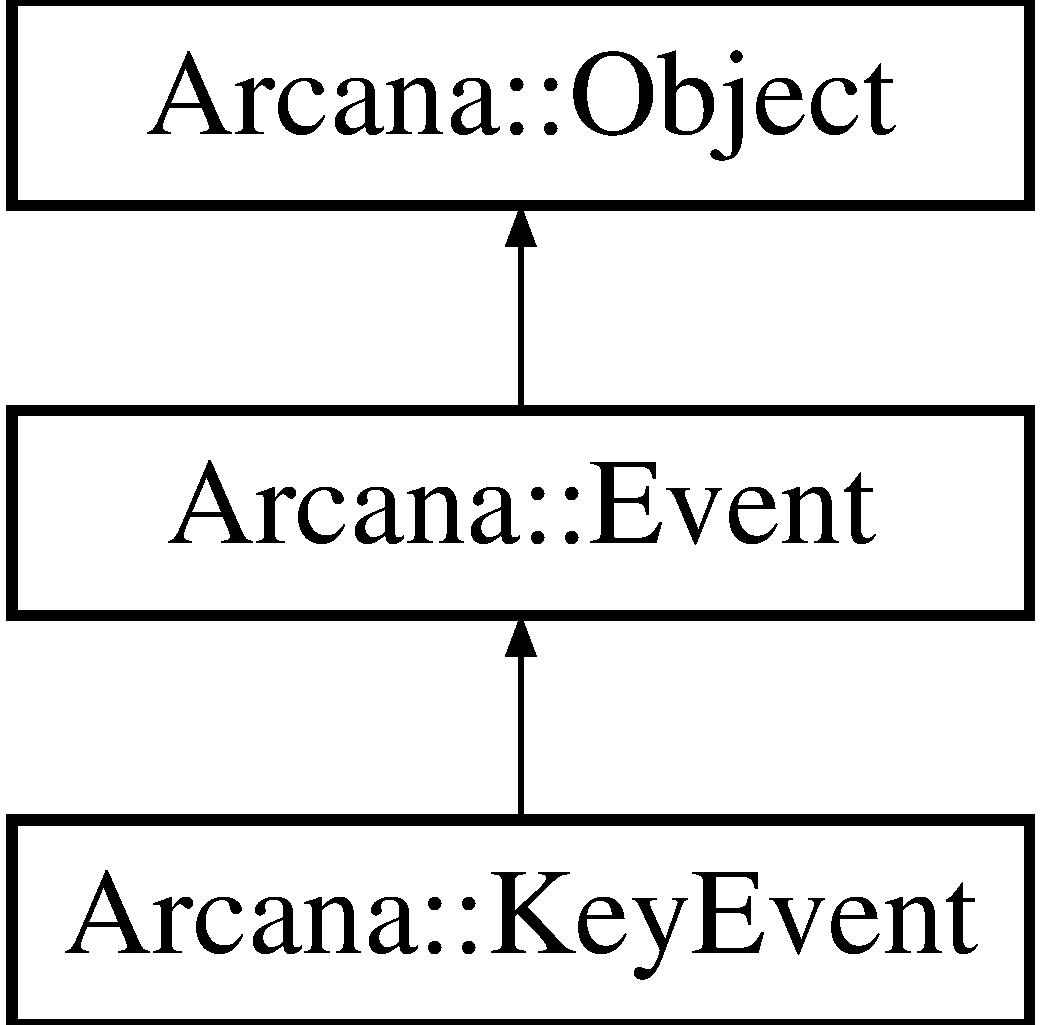
\includegraphics[height=3.000000cm]{class_arcana_1_1_key_event}
\end{center}
\end{figure}
\subsection*{Public Types}
\begin{DoxyCompactItemize}
\item 
enum \mbox{\hyperlink{class_arcana_1_1_key_event_a7e61abd92e372f41647951e8216a93e2}{Type}} \{ \mbox{\hyperlink{class_arcana_1_1_key_event_a7e61abd92e372f41647951e8216a93e2a2b1a00bb9a7e9413f0e672e8c9506153}{Pressed}}, 
\mbox{\hyperlink{class_arcana_1_1_key_event_a7e61abd92e372f41647951e8216a93e2a72cfc2d92b205338e06f3a8493960271}{Released}}, 
\mbox{\hyperlink{class_arcana_1_1_key_event_a7e61abd92e372f41647951e8216a93e2a3285127af15ec2c9ad551b174cd93d77}{Axis}}
 \}
\begin{DoxyCompactList}\small\item\em Enum defining the event type. \end{DoxyCompactList}\end{DoxyCompactItemize}
\subsection*{Public Member Functions}
\begin{DoxyCompactItemize}
\item 
\mbox{\Hypertarget{class_arcana_1_1_key_event_aaf2fd36768e5f3de12476fef5fa788d2}\label{class_arcana_1_1_key_event_aaf2fd36768e5f3de12476fef5fa788d2}} 
\mbox{\hyperlink{class_arcana_1_1_key_event_aaf2fd36768e5f3de12476fef5fa788d2}{Key\+Event}} (\mbox{\hyperlink{class_arcana_1_1_key_event_a7e61abd92e372f41647951e8216a93e2}{Type}} event, int32 key\+Code, bool alt=false, bool control=false, bool shift=false, bool system=false)
\begin{DoxyCompactList}\small\item\em \mbox{\hyperlink{class_arcana_1_1_key_event}{Key\+Event}} constructor. \end{DoxyCompactList}\item 
\mbox{\Hypertarget{class_arcana_1_1_key_event_a6478c87de863bbeb44386f602f6eceef}\label{class_arcana_1_1_key_event_a6478c87de863bbeb44386f602f6eceef}} 
\mbox{\hyperlink{class_arcana_1_1_key_event_a6478c87de863bbeb44386f602f6eceef}{Key\+Event}} (\mbox{\hyperlink{class_arcana_1_1_key_event_a7e61abd92e372f41647951e8216a93e2}{Type}} event, int32 key\+Code, int x, int y)
\begin{DoxyCompactList}\small\item\em \mbox{\hyperlink{class_arcana_1_1_key_event}{Key\+Event}} constructor. \end{DoxyCompactList}\item 
\mbox{\Hypertarget{class_arcana_1_1_key_event_ade909059da54ebe593df14f80f1c9d54}\label{class_arcana_1_1_key_event_ade909059da54ebe593df14f80f1c9d54}} 
\mbox{\hyperlink{class_arcana_1_1_key_event_ade909059da54ebe593df14f80f1c9d54}{Key\+Event}} (\mbox{\hyperlink{class_arcana_1_1_key_event_a7e61abd92e372f41647951e8216a93e2}{Type}} event, int32 controller\+Id, int32 key\+Code)
\begin{DoxyCompactList}\small\item\em \mbox{\hyperlink{class_arcana_1_1_key_event}{Key\+Event}} constructor for controller key presses. \end{DoxyCompactList}\item 
\mbox{\Hypertarget{class_arcana_1_1_key_event_a8af4057b5fba876cbee35c9f8901808e}\label{class_arcana_1_1_key_event_a8af4057b5fba876cbee35c9f8901808e}} 
\mbox{\hyperlink{class_arcana_1_1_key_event_a8af4057b5fba876cbee35c9f8901808e}{Key\+Event}} (int32 controller\+Id, int32 key\+Code, float axis)
\begin{DoxyCompactList}\small\item\em \mbox{\hyperlink{class_arcana_1_1_key_event}{Key\+Event}} constructor for controller axis keys. \end{DoxyCompactList}\item 
\mbox{\Hypertarget{class_arcana_1_1_key_event_a0c6ab0be338751bb466c1314c35976a2}\label{class_arcana_1_1_key_event_a0c6ab0be338751bb466c1314c35976a2}} 
\mbox{\hyperlink{class_arcana_1_1_key_event_a0c6ab0be338751bb466c1314c35976a2}{Key\+Event}} (int32 key\+Code, float axis)
\begin{DoxyCompactList}\small\item\em \mbox{\hyperlink{class_arcana_1_1_key_event}{Key\+Event}} constructor for axis keys. \end{DoxyCompactList}\end{DoxyCompactItemize}


\subsection{Detailed Description}
\mbox{\hyperlink{class_arcana_1_1_event}{Event}} broadcasted on key presses/releases. 

Key\+Events have and event id of 1. 

\subsection{Member Enumeration Documentation}
\mbox{\Hypertarget{class_arcana_1_1_key_event_a7e61abd92e372f41647951e8216a93e2}\label{class_arcana_1_1_key_event_a7e61abd92e372f41647951e8216a93e2}} 
\index{Arcana\+::\+Key\+Event@{Arcana\+::\+Key\+Event}!Type@{Type}}
\index{Type@{Type}!Arcana\+::\+Key\+Event@{Arcana\+::\+Key\+Event}}
\subsubsection{\texorpdfstring{Type}{Type}}
{\footnotesize\ttfamily enum \mbox{\hyperlink{class_arcana_1_1_key_event_a7e61abd92e372f41647951e8216a93e2}{Arcana\+::\+Key\+Event\+::\+Type}}}



Enum defining the event type. 

\begin{DoxyEnumFields}{Enumerator}
\raisebox{\heightof{T}}[0pt][0pt]{\index{Pressed@{Pressed}!Arcana\+::\+Key\+Event@{Arcana\+::\+Key\+Event}}\index{Arcana\+::\+Key\+Event@{Arcana\+::\+Key\+Event}!Pressed@{Pressed}}}\mbox{\Hypertarget{class_arcana_1_1_key_event_a7e61abd92e372f41647951e8216a93e2a2b1a00bb9a7e9413f0e672e8c9506153}\label{class_arcana_1_1_key_event_a7e61abd92e372f41647951e8216a93e2a2b1a00bb9a7e9413f0e672e8c9506153}} 
Pressed&Key was pressed. \\
\hline

\raisebox{\heightof{T}}[0pt][0pt]{\index{Released@{Released}!Arcana\+::\+Key\+Event@{Arcana\+::\+Key\+Event}}\index{Arcana\+::\+Key\+Event@{Arcana\+::\+Key\+Event}!Released@{Released}}}\mbox{\Hypertarget{class_arcana_1_1_key_event_a7e61abd92e372f41647951e8216a93e2a72cfc2d92b205338e06f3a8493960271}\label{class_arcana_1_1_key_event_a7e61abd92e372f41647951e8216a93e2a72cfc2d92b205338e06f3a8493960271}} 
Released&Key was released. \\
\hline

\raisebox{\heightof{T}}[0pt][0pt]{\index{Axis@{Axis}!Arcana\+::\+Key\+Event@{Arcana\+::\+Key\+Event}}\index{Arcana\+::\+Key\+Event@{Arcana\+::\+Key\+Event}!Axis@{Axis}}}\mbox{\Hypertarget{class_arcana_1_1_key_event_a7e61abd92e372f41647951e8216a93e2a3285127af15ec2c9ad551b174cd93d77}\label{class_arcana_1_1_key_event_a7e61abd92e372f41647951e8216a93e2a3285127af15ec2c9ad551b174cd93d77}} 
Axis&Key is an axis. \\
\hline

\end{DoxyEnumFields}


The documentation for this class was generated from the following file\+:\begin{DoxyCompactItemize}
\item 
Key\+Event.\+h\end{DoxyCompactItemize}

\hypertarget{struct_arcana_1_1_key_value_pair}{}\section{Arcana\+:\+:Key\+Value\+Pair$<$ Key\+Type, Value\+Type $>$ Struct Template Reference}
\label{struct_arcana_1_1_key_value_pair}\index{Arcana\+::\+Key\+Value\+Pair$<$ Key\+Type, Value\+Type $>$@{Arcana\+::\+Key\+Value\+Pair$<$ Key\+Type, Value\+Type $>$}}


Key/value pairs that are easy to use with custom containers. This class acts the same as the standard pair.  




{\ttfamily \#include $<$Arcana\+Template.\+h$>$}

\subsection*{Public Member Functions}
\begin{DoxyCompactItemize}
\item 
\mbox{\Hypertarget{struct_arcana_1_1_key_value_pair_a180f322ac6a83c57e85a9537e48f149b}\label{struct_arcana_1_1_key_value_pair_a180f322ac6a83c57e85a9537e48f149b}} 
\mbox{\hyperlink{struct_arcana_1_1_key_value_pair_a180f322ac6a83c57e85a9537e48f149b}{Key\+Value\+Pair}} (const Key\+Type \&In\+Key, const Value\+Type \&In\+Value)
\begin{DoxyCompactList}\small\item\em Constructor taking a key and a value. \end{DoxyCompactList}\item 
\mbox{\Hypertarget{struct_arcana_1_1_key_value_pair_a8d98e04c3d52554efd8734dfa966298a}\label{struct_arcana_1_1_key_value_pair_a8d98e04c3d52554efd8734dfa966298a}} 
\mbox{\hyperlink{struct_arcana_1_1_key_value_pair_a8d98e04c3d52554efd8734dfa966298a}{Key\+Value\+Pair}} (const Key\+Type \&In\+Key)
\begin{DoxyCompactList}\small\item\em Constructor taking just a key. Creates a pair with an uninitialized value. \end{DoxyCompactList}\item 
\mbox{\Hypertarget{struct_arcana_1_1_key_value_pair_a039e3a478d84fdcd72e5f50eea76eb67}\label{struct_arcana_1_1_key_value_pair_a039e3a478d84fdcd72e5f50eea76eb67}} 
\mbox{\hyperlink{struct_arcana_1_1_key_value_pair_a039e3a478d84fdcd72e5f50eea76eb67}{Key\+Value\+Pair}} ()
\begin{DoxyCompactList}\small\item\em Default constructor. Creates a pair with an uninitialized key and an uninitialized value. \end{DoxyCompactList}\item 
\mbox{\Hypertarget{struct_arcana_1_1_key_value_pair_a8c1603f71f89893505fde564ca3979b2}\label{struct_arcana_1_1_key_value_pair_a8c1603f71f89893505fde564ca3979b2}} 
bool \mbox{\hyperlink{struct_arcana_1_1_key_value_pair_a8c1603f71f89893505fde564ca3979b2}{operator==}} (const \mbox{\hyperlink{struct_arcana_1_1_key_value_pair}{Key\+Value\+Pair}} \&other) const
\begin{DoxyCompactList}\small\item\em Equals operator. Only checks key equality. \end{DoxyCompactList}\item 
\mbox{\Hypertarget{struct_arcana_1_1_key_value_pair_a4998b66f9f46840ed34a38f7eac61de3}\label{struct_arcana_1_1_key_value_pair_a4998b66f9f46840ed34a38f7eac61de3}} 
bool \mbox{\hyperlink{struct_arcana_1_1_key_value_pair_a4998b66f9f46840ed34a38f7eac61de3}{operator!=}} (const \mbox{\hyperlink{struct_arcana_1_1_key_value_pair}{Key\+Value\+Pair}} \&other) const
\begin{DoxyCompactList}\small\item\em Inequality operator. Only checks key inequality. \end{DoxyCompactList}\item 
\mbox{\Hypertarget{struct_arcana_1_1_key_value_pair_a83febe1b51b6e4045a4c20a6e3b1b716}\label{struct_arcana_1_1_key_value_pair_a83febe1b51b6e4045a4c20a6e3b1b716}} 
bool \mbox{\hyperlink{struct_arcana_1_1_key_value_pair_a83febe1b51b6e4045a4c20a6e3b1b716}{operator$<$}} (const \mbox{\hyperlink{struct_arcana_1_1_key_value_pair}{Key\+Value\+Pair}} \&other) const
\begin{DoxyCompactList}\small\item\em Less than operator. Only checks if this key is less than the other key. \end{DoxyCompactList}\item 
\mbox{\Hypertarget{struct_arcana_1_1_key_value_pair_a510a057a546badb0bb02c88dfa61ad15}\label{struct_arcana_1_1_key_value_pair_a510a057a546badb0bb02c88dfa61ad15}} 
bool \mbox{\hyperlink{struct_arcana_1_1_key_value_pair_a510a057a546badb0bb02c88dfa61ad15}{operator()}} (const \mbox{\hyperlink{struct_arcana_1_1_key_value_pair}{Key\+Value\+Pair}} \&A, const \mbox{\hyperlink{struct_arcana_1_1_key_value_pair}{Key\+Value\+Pair}} \&B) const
\begin{DoxyCompactList}\small\item\em Functor operator taking two different Key\+Value\+Pairs. Checks if this key is less than the other key. \end{DoxyCompactList}\end{DoxyCompactItemize}
\subsection*{Public Attributes}
\begin{DoxyCompactItemize}
\item 
\mbox{\Hypertarget{struct_arcana_1_1_key_value_pair_a7fb93bbd899926462e6504bf1b433089}\label{struct_arcana_1_1_key_value_pair_a7fb93bbd899926462e6504bf1b433089}} 
Key\+Type {\bfseries key}
\item 
\mbox{\Hypertarget{struct_arcana_1_1_key_value_pair_a79ee05436469e504508ca0597920c77a}\label{struct_arcana_1_1_key_value_pair_a79ee05436469e504508ca0597920c77a}} 
Value\+Type {\bfseries value}
\end{DoxyCompactItemize}


\subsection{Detailed Description}
\subsubsection*{template$<$typename Key\+Type, typename Value\+Type$>$\newline
struct Arcana\+::\+Key\+Value\+Pair$<$ Key\+Type, Value\+Type $>$}

Key/value pairs that are easy to use with custom containers. This class acts the same as the standard pair. 

The documentation for this struct was generated from the following file\+:\begin{DoxyCompactItemize}
\item 
Arcana\+Template.\+h\end{DoxyCompactItemize}

\hypertarget{class_arcana_1_1_member_function_callback_instance}{}\section{Arcana\+:\+:Member\+Function\+Callback\+Instance$<$ Object\+Type, Return\+Value, Argument\+Types $>$ Class Template Reference}
\label{class_arcana_1_1_member_function_callback_instance}\index{Arcana\+::\+Member\+Function\+Callback\+Instance$<$ Object\+Type, Return\+Value, Argument\+Types $>$@{Arcana\+::\+Member\+Function\+Callback\+Instance$<$ Object\+Type, Return\+Value, Argument\+Types $>$}}


Callback instance wrapping a member function pointer.  




{\ttfamily \#include $<$Member\+Function\+Callback\+Instance.\+h$>$}

Inheritance diagram for Arcana\+:\+:Member\+Function\+Callback\+Instance$<$ Object\+Type, Return\+Value, Argument\+Types $>$\+:\begin{figure}[H]
\begin{center}
\leavevmode
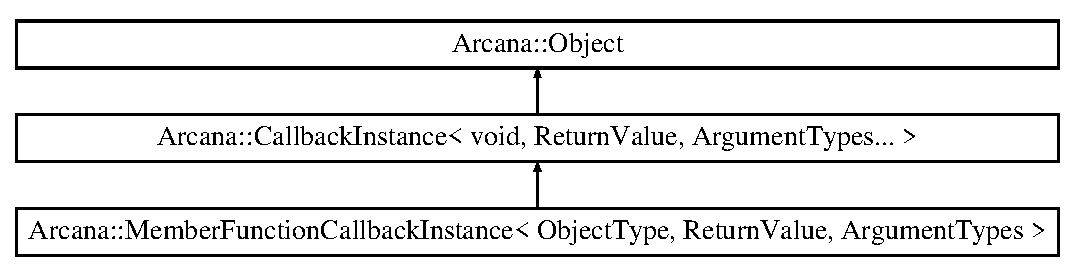
\includegraphics[height=3.000000cm]{class_arcana_1_1_member_function_callback_instance}
\end{center}
\end{figure}
\subsection*{Public Types}
\begin{DoxyCompactItemize}
\item 
\mbox{\Hypertarget{class_arcana_1_1_member_function_callback_instance_ad7ba7b4937f6301718e8dffb89068f20}\label{class_arcana_1_1_member_function_callback_instance_ad7ba7b4937f6301718e8dffb89068f20}} 
typedef Return\+Value(Object\+Type\+::$\ast$ \mbox{\hyperlink{class_arcana_1_1_member_function_callback_instance_ad7ba7b4937f6301718e8dffb89068f20}{Callback\+Function}}) (Argument\+Types...)
\begin{DoxyCompactList}\small\item\em Function pointer typedef. \end{DoxyCompactList}\end{DoxyCompactItemize}
\subsection*{Public Member Functions}
\begin{DoxyCompactItemize}
\item 
virtual Return\+Value \mbox{\hyperlink{class_arcana_1_1_member_function_callback_instance_aa3da0ee51ae4a6465844c7af67da7d83}{execute}} (Argument\+Types \&\&... args) override
\begin{DoxyCompactList}\small\item\em Executes the function. \end{DoxyCompactList}\item 
virtual Return\+Value \mbox{\hyperlink{class_arcana_1_1_member_function_callback_instance_a4d8c12162b9d7b42ad9916d2dba5327d}{execute\+If\+Bound}} (Argument\+Types \&\&... args) override
\begin{DoxyCompactList}\small\item\em Executes the function. \end{DoxyCompactList}\item 
\mbox{\Hypertarget{class_arcana_1_1_member_function_callback_instance_ae9c3a3e3a3b8722c34b1133763a8227b}\label{class_arcana_1_1_member_function_callback_instance_ae9c3a3e3a3b8722c34b1133763a8227b}} 
virtual bool \mbox{\hyperlink{class_arcana_1_1_member_function_callback_instance_ae9c3a3e3a3b8722c34b1133763a8227b}{is\+Bound}} () override
\begin{DoxyCompactList}\small\item\em Returns true if a function pointer is bound. \end{DoxyCompactList}\item 
\mbox{\Hypertarget{class_arcana_1_1_member_function_callback_instance_aa15906d8500efc0ba749a7390748eeb7}\label{class_arcana_1_1_member_function_callback_instance_aa15906d8500efc0ba749a7390748eeb7}} 
virtual bool \mbox{\hyperlink{class_arcana_1_1_member_function_callback_instance_aa15906d8500efc0ba749a7390748eeb7}{is\+Static\+Function}} () const override
\begin{DoxyCompactList}\small\item\em Returns true if a function is a static function. \end{DoxyCompactList}\item 
\mbox{\Hypertarget{class_arcana_1_1_member_function_callback_instance_a9cafc44cbe8d2df52ca94d516f9809ba}\label{class_arcana_1_1_member_function_callback_instance_a9cafc44cbe8d2df52ca94d516f9809ba}} 
virtual void \mbox{\hyperlink{class_arcana_1_1_member_function_callback_instance_a9cafc44cbe8d2df52ca94d516f9809ba}{unbind}} () override
\begin{DoxyCompactList}\small\item\em Sets the object and function pointer members to null. \end{DoxyCompactList}\item 
virtual void \mbox{\hyperlink{class_arcana_1_1_member_function_callback_instance_ae93ba2e166f268d480431bb7dfd00140}{bind}} (void $\ast$object, void(Object\+::$\ast$function)()) override
\begin{DoxyCompactList}\small\item\em Binds this callback to the member function of an object. \end{DoxyCompactList}\end{DoxyCompactItemize}
\subsection*{Public Attributes}
\begin{DoxyCompactItemize}
\item 
\mbox{\Hypertarget{class_arcana_1_1_member_function_callback_instance_a2ec153b43407b049f27d012df6d8c4f4}\label{class_arcana_1_1_member_function_callback_instance_a2ec153b43407b049f27d012df6d8c4f4}} 
Object\+Type $\ast$ {\bfseries \+\_\+object}
\item 
\mbox{\Hypertarget{class_arcana_1_1_member_function_callback_instance_a4eb431b612dddd4e03da01e57894bbb2}\label{class_arcana_1_1_member_function_callback_instance_a4eb431b612dddd4e03da01e57894bbb2}} 
\mbox{\hyperlink{class_arcana_1_1_member_function_callback_instance_ad7ba7b4937f6301718e8dffb89068f20}{Callback\+Function}} {\bfseries \+\_\+function}
\end{DoxyCompactItemize}


\subsection{Detailed Description}
\subsubsection*{template$<$typename Object\+Type, typename Return\+Value, typename... Argument\+Types$>$\newline
class Arcana\+::\+Member\+Function\+Callback\+Instance$<$ Object\+Type, Return\+Value, Argument\+Types $>$}

Callback instance wrapping a member function pointer. 

Needs to be bound to a function pointer and an object. 

\subsection{Member Function Documentation}
\mbox{\Hypertarget{class_arcana_1_1_member_function_callback_instance_ae93ba2e166f268d480431bb7dfd00140}\label{class_arcana_1_1_member_function_callback_instance_ae93ba2e166f268d480431bb7dfd00140}} 
\index{Arcana\+::\+Member\+Function\+Callback\+Instance@{Arcana\+::\+Member\+Function\+Callback\+Instance}!bind@{bind}}
\index{bind@{bind}!Arcana\+::\+Member\+Function\+Callback\+Instance@{Arcana\+::\+Member\+Function\+Callback\+Instance}}
\subsubsection{\texorpdfstring{bind()}{bind()}}
{\footnotesize\ttfamily template$<$typename Object\+Type , typename Return\+Value , typename... Argument\+Types$>$ \\
virtual void \mbox{\hyperlink{class_arcana_1_1_member_function_callback_instance}{Arcana\+::\+Member\+Function\+Callback\+Instance}}$<$ Object\+Type, Return\+Value, Argument\+Types $>$\+::bind (\begin{DoxyParamCaption}\item[{void $\ast$}]{object,  }\item[{void(Object\+::$\ast$)()}]{ }\end{DoxyParamCaption})\hspace{0.3cm}{\ttfamily [inline]}, {\ttfamily [override]}, {\ttfamily [virtual]}}



Binds this callback to the member function of an object. 

The member function must take the arguments specified in the \mbox{\hyperlink{class_arcana_1_1_callback_instance}{Callback\+Instance}} templates. 

Reimplemented from \mbox{\hyperlink{class_arcana_1_1_callback_instance_a55e87e320e0133a4274c60e87a391a7e}{Arcana\+::\+Callback\+Instance$<$ void, Return\+Value, Argument\+Types... $>$}}.

\mbox{\Hypertarget{class_arcana_1_1_member_function_callback_instance_aa3da0ee51ae4a6465844c7af67da7d83}\label{class_arcana_1_1_member_function_callback_instance_aa3da0ee51ae4a6465844c7af67da7d83}} 
\index{Arcana\+::\+Member\+Function\+Callback\+Instance@{Arcana\+::\+Member\+Function\+Callback\+Instance}!execute@{execute}}
\index{execute@{execute}!Arcana\+::\+Member\+Function\+Callback\+Instance@{Arcana\+::\+Member\+Function\+Callback\+Instance}}
\subsubsection{\texorpdfstring{execute()}{execute()}}
{\footnotesize\ttfamily template$<$typename Object\+Type , typename Return\+Value , typename... Argument\+Types$>$ \\
virtual Return\+Value \mbox{\hyperlink{class_arcana_1_1_member_function_callback_instance}{Arcana\+::\+Member\+Function\+Callback\+Instance}}$<$ Object\+Type, Return\+Value, Argument\+Types $>$\+::execute (\begin{DoxyParamCaption}\item[{Argument\+Types \&\&...}]{args }\end{DoxyParamCaption})\hspace{0.3cm}{\ttfamily [inline]}, {\ttfamily [override]}, {\ttfamily [virtual]}}



Executes the function. 

An unknown number of arguments can be passed. The argument types must coincide with the initial arguments specified in the template. 

Implements \mbox{\hyperlink{class_arcana_1_1_callback_instance_aa5bd9b4ee2129a0c22a98f7fa1cfc724}{Arcana\+::\+Callback\+Instance$<$ void, Return\+Value, Argument\+Types... $>$}}.

\mbox{\Hypertarget{class_arcana_1_1_member_function_callback_instance_a4d8c12162b9d7b42ad9916d2dba5327d}\label{class_arcana_1_1_member_function_callback_instance_a4d8c12162b9d7b42ad9916d2dba5327d}} 
\index{Arcana\+::\+Member\+Function\+Callback\+Instance@{Arcana\+::\+Member\+Function\+Callback\+Instance}!execute\+If\+Bound@{execute\+If\+Bound}}
\index{execute\+If\+Bound@{execute\+If\+Bound}!Arcana\+::\+Member\+Function\+Callback\+Instance@{Arcana\+::\+Member\+Function\+Callback\+Instance}}
\subsubsection{\texorpdfstring{execute\+If\+Bound()}{executeIfBound()}}
{\footnotesize\ttfamily template$<$typename Object\+Type , typename Return\+Value , typename... Argument\+Types$>$ \\
virtual Return\+Value \mbox{\hyperlink{class_arcana_1_1_member_function_callback_instance}{Arcana\+::\+Member\+Function\+Callback\+Instance}}$<$ Object\+Type, Return\+Value, Argument\+Types $>$\+::execute\+If\+Bound (\begin{DoxyParamCaption}\item[{Argument\+Types \&\&...}]{args }\end{DoxyParamCaption})\hspace{0.3cm}{\ttfamily [inline]}, {\ttfamily [override]}, {\ttfamily [virtual]}}



Executes the function. 

An unknown number of arguments can be passed. The argument types must coincide with the initial arguments specified in the template. This method is the same as \mbox{\hyperlink{class_arcana_1_1_member_function_callback_instance_aa3da0ee51ae4a6465844c7af67da7d83}{execute()}}, but without the assertion. 

Implements \mbox{\hyperlink{class_arcana_1_1_callback_instance_af4aced5d787cabb857931ecd87c3ab50}{Arcana\+::\+Callback\+Instance$<$ void, Return\+Value, Argument\+Types... $>$}}.



The documentation for this class was generated from the following file\+:\begin{DoxyCompactItemize}
\item 
Member\+Function\+Callback\+Instance.\+h\end{DoxyCompactItemize}

\hypertarget{class_arcana_1_1_memory}{}\section{Arcana\+:\+:Memory Class Reference}
\label{class_arcana_1_1_memory}\index{Arcana\+::\+Memory@{Arcana\+::\+Memory}}


Handles memory allocations. This class wraps platform-\/specific memory operations and provides simple memory management methods.  




{\ttfamily \#include $<$Arcana\+Memory.\+h$>$}

\subsection*{Public Types}
\begin{DoxyCompactItemize}
\item 
\mbox{\Hypertarget{class_arcana_1_1_memory_af973bacdc73996a616bbd9dc20971a35}\label{class_arcana_1_1_memory_af973bacdc73996a616bbd9dc20971a35}} 
enum \{ {\bfseries D\+E\+F\+A\+U\+L\+T\+\_\+\+A\+L\+I\+G\+N\+M\+E\+NT} = 0, 
{\bfseries M\+I\+N\+\_\+\+A\+L\+I\+G\+N\+M\+E\+NT} = 8
 \}
\end{DoxyCompactItemize}
\subsection*{Static Public Member Functions}
\begin{DoxyCompactItemize}
\item 
\mbox{\Hypertarget{class_arcana_1_1_memory_aeb97706378a7193a45903247e318e061}\label{class_arcana_1_1_memory_aeb97706378a7193a45903247e318e061}} 
static void $\ast$ {\bfseries memmove} (void $\ast$dest, const void $\ast$src, size\+\_\+t count)
\item 
\mbox{\Hypertarget{class_arcana_1_1_memory_aaa86ed29dadc7b727e9095d61c02df99}\label{class_arcana_1_1_memory_aaa86ed29dadc7b727e9095d61c02df99}} 
static int32 {\bfseries memcmp} (const void $\ast$buf1, const void $\ast$buf2, size\+\_\+t count)
\item 
\mbox{\Hypertarget{class_arcana_1_1_memory_a55b4b6d7d9ac83f2def9173ace8a1e3f}\label{class_arcana_1_1_memory_a55b4b6d7d9ac83f2def9173ace8a1e3f}} 
static void $\ast$ {\bfseries memset} (void $\ast$dest, uint8 ch, size\+\_\+t count)
\item 
\mbox{\Hypertarget{class_arcana_1_1_memory_a35209e6ffc57590e0edbb99022bad463}\label{class_arcana_1_1_memory_a35209e6ffc57590e0edbb99022bad463}} 
{\footnotesize template$<$class T $>$ }\\static void {\bfseries memset} (T \&src, uint8 value)
\item 
\mbox{\Hypertarget{class_arcana_1_1_memory_ad21b6b9e99dec42df69c4faf409976e8}\label{class_arcana_1_1_memory_ad21b6b9e99dec42df69c4faf409976e8}} 
static void $\ast$ {\bfseries memzero} (void $\ast$dest, size\+\_\+t count)
\item 
\mbox{\Hypertarget{class_arcana_1_1_memory_a9e1a518ad0cf1375ce1888205e618451}\label{class_arcana_1_1_memory_a9e1a518ad0cf1375ce1888205e618451}} 
{\footnotesize template$<$class T $>$ }\\static void {\bfseries memzero} (T \&src)
\item 
\mbox{\Hypertarget{class_arcana_1_1_memory_aa17424bed341eeb0dd05d6d01878a769}\label{class_arcana_1_1_memory_aa17424bed341eeb0dd05d6d01878a769}} 
static void $\ast$ {\bfseries memcpy} (void $\ast$dest, const void $\ast$src, size\+\_\+t count)
\item 
\mbox{\Hypertarget{class_arcana_1_1_memory_a44d141c4ace622535407d8bedd430bd4}\label{class_arcana_1_1_memory_a44d141c4ace622535407d8bedd430bd4}} 
{\footnotesize template$<$class T $>$ }\\static void {\bfseries memcpy} (T \&dest, const T \&src)
\item 
\mbox{\Hypertarget{class_arcana_1_1_memory_a1cd99f9cd97ff110c5fa9aacaf4eded6}\label{class_arcana_1_1_memory_a1cd99f9cd97ff110c5fa9aacaf4eded6}} 
static void $\ast$ {\bfseries bigblock\+Memcpy} (void $\ast$dest, const void $\ast$src, size\+\_\+t count)
\item 
\mbox{\Hypertarget{class_arcana_1_1_memory_ac3bf58e7eb9702b5b9706e1bde1ecaf1}\label{class_arcana_1_1_memory_ac3bf58e7eb9702b5b9706e1bde1ecaf1}} 
static void $\ast$ {\bfseries streaming\+Memcpy} (void $\ast$dest, const void $\ast$src, size\+\_\+t count)
\item 
\mbox{\Hypertarget{class_arcana_1_1_memory_abc0042b4b6f8f2680b28df7715c64a34}\label{class_arcana_1_1_memory_abc0042b4b6f8f2680b28df7715c64a34}} 
static void {\bfseries memswap} (void $\ast$ptr1, void $\ast$ptr2, size\+\_\+t size)
\item 
\mbox{\Hypertarget{class_arcana_1_1_memory_a1f71ef6a571f0812fa159eed696f2bd3}\label{class_arcana_1_1_memory_a1f71ef6a571f0812fa159eed696f2bd3}} 
static void $\ast$ {\bfseries system\+Malloc} (size\+\_\+t size)
\item 
\mbox{\Hypertarget{class_arcana_1_1_memory_aa08e74fbd0f7ffc1554819605a945113}\label{class_arcana_1_1_memory_aa08e74fbd0f7ffc1554819605a945113}} 
static void {\bfseries system\+Free} (void $\ast$ptr)
\item 
\mbox{\Hypertarget{class_arcana_1_1_memory_a320eb10834e1d1b45af0bf7c75931c28}\label{class_arcana_1_1_memory_a320eb10834e1d1b45af0bf7c75931c28}} 
static void $\ast$ {\bfseries malloc} (size\+\_\+t count, uint32 alignment=D\+E\+F\+A\+U\+L\+T\+\_\+\+A\+L\+I\+G\+N\+M\+E\+NT)
\item 
\mbox{\Hypertarget{class_arcana_1_1_memory_a55e4cfcfb71508be2fab37efb5d4b720}\label{class_arcana_1_1_memory_a55e4cfcfb71508be2fab37efb5d4b720}} 
static void $\ast$ {\bfseries realloc} (void $\ast$original, size\+\_\+t count, uint32 alignment=D\+E\+F\+A\+U\+L\+T\+\_\+\+A\+L\+I\+G\+N\+M\+E\+NT)
\item 
\mbox{\Hypertarget{class_arcana_1_1_memory_a4cf60312bc57041b3423a693c7258f42}\label{class_arcana_1_1_memory_a4cf60312bc57041b3423a693c7258f42}} 
static void {\bfseries free} (void $\ast$original)
\item 
\mbox{\Hypertarget{class_arcana_1_1_memory_a449fecd7c0eabe7d1f02135c6c2e86e1}\label{class_arcana_1_1_memory_a449fecd7c0eabe7d1f02135c6c2e86e1}} 
static size\+\_\+t {\bfseries get\+Alloc\+Size} (void $\ast$original)
\item 
\mbox{\Hypertarget{class_arcana_1_1_memory_af433a0e9faeb7db992445709016118c3}\label{class_arcana_1_1_memory_af433a0e9faeb7db992445709016118c3}} 
{\footnotesize template$<$typename Element\+Type $>$ }\\static \mbox{\hyperlink{class_arcana_1_1_enable_if}{Enable\+If}}$<$ \mbox{\hyperlink{struct_arcana_1_1_type_traits}{Type\+Traits}}$<$ Element\+Type $>$\+::Needs\+Destructor $>$\+::\mbox{\hyperlink{class_arcana_1_1_type}{Type}} {\bfseries destruct\+Items} (Element\+Type $\ast$element, int32 count)
\item 
\mbox{\Hypertarget{class_arcana_1_1_memory_a5d289f8e15bd3e79116e4371db48231c}\label{class_arcana_1_1_memory_a5d289f8e15bd3e79116e4371db48231c}} 
{\footnotesize template$<$typename Element\+Type $>$ }\\static \mbox{\hyperlink{class_arcana_1_1_enable_if}{Enable\+If}}$<$!\mbox{\hyperlink{struct_arcana_1_1_type_traits}{Type\+Traits}}$<$ Element\+Type $>$\+::Needs\+Destructor $>$\+::\mbox{\hyperlink{class_arcana_1_1_type}{Type}} {\bfseries destruct\+Items} (Element\+Type $\ast$elements, int32 count)
\item 
\mbox{\Hypertarget{class_arcana_1_1_memory_a00781002e3490042ba907779902cbe5e}\label{class_arcana_1_1_memory_a00781002e3490042ba907779902cbe5e}} 
{\footnotesize template$<$typename Destination\+Element\+Type , typename Source\+Element\+Type $>$ }\\static void {\bfseries construct\+Items} (void $\ast$dest, const Source\+Element\+Type $\ast$source, int32 count)
\item 
\mbox{\Hypertarget{class_arcana_1_1_memory_af8cd6cb4c679e43ebdb1d7343e01ac49}\label{class_arcana_1_1_memory_af8cd6cb4c679e43ebdb1d7343e01ac49}} 
{\footnotesize template$<$typename Element\+Type $>$ }\\static \mbox{\hyperlink{class_arcana_1_1_enable_if}{Enable\+If}}$<$!\mbox{\hyperlink{struct_arcana_1_1_type_traits}{Type\+Traits}}$<$ Element\+Type $>$\+::Is\+Zero\+Construct\+Type $>$\+::\mbox{\hyperlink{class_arcana_1_1_type}{Type}} {\bfseries default\+Construct\+Items} (void $\ast$Address, int32 Count)
\item 
\mbox{\Hypertarget{class_arcana_1_1_memory_a1dbdd5b76307b840d183370a6c10df6a}\label{class_arcana_1_1_memory_a1dbdd5b76307b840d183370a6c10df6a}} 
{\footnotesize template$<$typename Element\+Type $>$ }\\static \mbox{\hyperlink{class_arcana_1_1_enable_if}{Enable\+If}}$<$ \mbox{\hyperlink{struct_arcana_1_1_type_traits}{Type\+Traits}}$<$ Element\+Type $>$\+::Is\+Zero\+Construct\+Type $>$\+::\mbox{\hyperlink{class_arcana_1_1_type}{Type}} {\bfseries default\+Construct\+Items} (void $\ast$elements, int32 count)
\item 
\mbox{\Hypertarget{class_arcana_1_1_memory_ab3cfef6ea5391ccbb532bea2826b0b04}\label{class_arcana_1_1_memory_ab3cfef6ea5391ccbb532bea2826b0b04}} 
{\footnotesize template$<$typename Destination\+Element\+Type , typename Source\+Element\+Type $>$ }\\static void {\bfseries relocate\+Construct\+Items} (void $\ast$dest, const Source\+Element\+Type $\ast$source, int32 count)
\end{DoxyCompactItemize}


\subsection{Detailed Description}
Handles memory allocations. This class wraps platform-\/specific memory operations and provides simple memory management methods. 

The documentation for this class was generated from the following files\+:\begin{DoxyCompactItemize}
\item 
Arcana\+Memory.\+h\item 
Arcana\+Memory.\+cpp\end{DoxyCompactItemize}

\hypertarget{class_arcana_1_1_memory_allocator}{}\section{Arcana\+:\+:Memory\+Allocator Class Reference}
\label{class_arcana_1_1_memory_allocator}\index{Arcana\+::\+Memory\+Allocator@{Arcana\+::\+Memory\+Allocator}}
\subsection*{Classes}
\begin{DoxyCompactItemize}
\item 
struct \mbox{\hyperlink{struct_arcana_1_1_memory_allocator_1_1_unknown_type}{Unknown\+Type}}
\end{DoxyCompactItemize}
\subsection*{Public Member Functions}
\begin{DoxyCompactItemize}
\item 
\mbox{\Hypertarget{class_arcana_1_1_memory_allocator_ad666f3a8253e8db9014312ea9e31f938}\label{class_arcana_1_1_memory_allocator_ad666f3a8253e8db9014312ea9e31f938}} 
void {\bfseries move\+To\+Empty} (\mbox{\hyperlink{class_arcana_1_1_memory_allocator}{Memory\+Allocator}} \&other)
\item 
\mbox{\Hypertarget{class_arcana_1_1_memory_allocator_a663af3a3a9eaa69f783c0b54fa151ec6}\label{class_arcana_1_1_memory_allocator_a663af3a3a9eaa69f783c0b54fa151ec6}} 
\mbox{\hyperlink{struct_arcana_1_1_memory_allocator_1_1_unknown_type}{Unknown\+Type}} $\ast$ {\bfseries get\+Allocation} () const
\item 
\mbox{\Hypertarget{class_arcana_1_1_memory_allocator_abd738971dc3566995442e1ad3a11950a}\label{class_arcana_1_1_memory_allocator_abd738971dc3566995442e1ad3a11950a}} 
void {\bfseries resize\+Allocation} (int32 previous\+Num\+Elements, int32 num\+Elements, size\+\_\+t num\+Bytes\+Per\+Element)
\item 
\mbox{\Hypertarget{class_arcana_1_1_memory_allocator_afd95c3951e887361cc76954db1e7197a}\label{class_arcana_1_1_memory_allocator_afd95c3951e887361cc76954db1e7197a}} 
int32 {\bfseries calculate\+Slack} (int32 num\+Elements, int32 num\+Allocated\+Elements, size\+\_\+t num\+Bytes\+Per\+Element) const
\item 
\mbox{\Hypertarget{class_arcana_1_1_memory_allocator_ab162927b3e2a3c594ac21f8cc1491cca}\label{class_arcana_1_1_memory_allocator_ab162927b3e2a3c594ac21f8cc1491cca}} 
size\+\_\+t {\bfseries get\+Allocated\+Size} (int32 num\+Allocated\+Elements, size\+\_\+t num\+Bytes\+Per\+Element) const
\end{DoxyCompactItemize}


The documentation for this class was generated from the following files\+:\begin{DoxyCompactItemize}
\item 
Memory\+Allocator.\+h\item 
Memory\+Allocator.\+cpp\end{DoxyCompactItemize}

\hypertarget{class_arcana_1_1_message}{}\section{Arcana\+:\+:Message Class Reference}
\label{class_arcana_1_1_message}\index{Arcana\+::\+Message@{Arcana\+::\+Message}}


This class manages the lifetime of an \mbox{\hyperlink{class_arcana_1_1_event}{Event}} pointer.  




{\ttfamily \#include $<$Message.\+h$>$}

\subsection*{Public Member Functions}
\begin{DoxyCompactItemize}
\item 
\mbox{\Hypertarget{class_arcana_1_1_message_ab3cbb035a75bbca7335238fc904cf685}\label{class_arcana_1_1_message_ab3cbb035a75bbca7335238fc904cf685}} 
\mbox{\hyperlink{class_arcana_1_1_message_ab3cbb035a75bbca7335238fc904cf685}{Message}} ()
\begin{DoxyCompactList}\small\item\em \mbox{\hyperlink{class_arcana_1_1_message}{Message}} default constructor. \end{DoxyCompactList}\item 
\mbox{\hyperlink{class_arcana_1_1_message_aca77fd2984b45c908631451d1ab29fa1}{Message}} (\mbox{\hyperlink{class_arcana_1_1_event}{Event}} $\ast$event)
\begin{DoxyCompactList}\small\item\em \mbox{\hyperlink{class_arcana_1_1_message}{Message}} event constructor. \end{DoxyCompactList}\item 
\mbox{\hyperlink{class_arcana_1_1_message_a4c1cb77c70947ff48b6f54f83b94e141}{Message}} (const \mbox{\hyperlink{class_arcana_1_1_message}{Message}} \&message)
\begin{DoxyCompactList}\small\item\em \mbox{\hyperlink{class_arcana_1_1_message}{Message}} copy constructor. \end{DoxyCompactList}\item 
\mbox{\hyperlink{class_arcana_1_1_message_a08fee1d23b404de28250cc3e61bdef6b}{$\sim$\+Message}} ()
\begin{DoxyCompactList}\small\item\em \mbox{\hyperlink{class_arcana_1_1_message}{Message}} destructor. \end{DoxyCompactList}\item 
\mbox{\Hypertarget{class_arcana_1_1_message_a467ff543095f62784bb96f0d47d5c534}\label{class_arcana_1_1_message_a467ff543095f62784bb96f0d47d5c534}} 
void \mbox{\hyperlink{class_arcana_1_1_message_a467ff543095f62784bb96f0d47d5c534}{set\+Event}} (\mbox{\hyperlink{class_arcana_1_1_event}{Event}} $\ast$event)
\begin{DoxyCompactList}\small\item\em Sets the event pointer. \end{DoxyCompactList}\item 
\mbox{\Hypertarget{class_arcana_1_1_message_a3144ea29e7d6690d739b6108a982682e}\label{class_arcana_1_1_message_a3144ea29e7d6690d739b6108a982682e}} 
\mbox{\hyperlink{class_arcana_1_1_event}{Event}} \& \mbox{\hyperlink{class_arcana_1_1_message_a3144ea29e7d6690d739b6108a982682e}{get\+Event}} ()
\begin{DoxyCompactList}\small\item\em Dereferences the event pointer. \end{DoxyCompactList}\item 
\mbox{\Hypertarget{class_arcana_1_1_message_ad95056caca487439a787772ae62de53e}\label{class_arcana_1_1_message_ad95056caca487439a787772ae62de53e}} 
\mbox{\hyperlink{class_arcana_1_1_message}{Message}} \& \mbox{\hyperlink{class_arcana_1_1_message_ad95056caca487439a787772ae62de53e}{operator=}} (const \mbox{\hyperlink{class_arcana_1_1_message}{Message}} \&msg)
\begin{DoxyCompactList}\small\item\em \mbox{\hyperlink{class_arcana_1_1_message}{Message}} assignment operator. \end{DoxyCompactList}\end{DoxyCompactItemize}


\subsection{Detailed Description}
This class manages the lifetime of an \mbox{\hyperlink{class_arcana_1_1_event}{Event}} pointer. 

\subsection{Constructor \& Destructor Documentation}
\mbox{\Hypertarget{class_arcana_1_1_message_aca77fd2984b45c908631451d1ab29fa1}\label{class_arcana_1_1_message_aca77fd2984b45c908631451d1ab29fa1}} 
\index{Arcana\+::\+Message@{Arcana\+::\+Message}!Message@{Message}}
\index{Message@{Message}!Arcana\+::\+Message@{Arcana\+::\+Message}}
\subsubsection{\texorpdfstring{Message()}{Message()}\hspace{0.1cm}{\footnotesize\ttfamily [1/2]}}
{\footnotesize\ttfamily Arcana\+::\+Message\+::\+Message (\begin{DoxyParamCaption}\item[{\mbox{\hyperlink{class_arcana_1_1_event}{Event}} $\ast$}]{event }\end{DoxyParamCaption})}



\mbox{\hyperlink{class_arcana_1_1_message}{Message}} event constructor. 

References and stores the event pointer. \mbox{\Hypertarget{class_arcana_1_1_message_a4c1cb77c70947ff48b6f54f83b94e141}\label{class_arcana_1_1_message_a4c1cb77c70947ff48b6f54f83b94e141}} 
\index{Arcana\+::\+Message@{Arcana\+::\+Message}!Message@{Message}}
\index{Message@{Message}!Arcana\+::\+Message@{Arcana\+::\+Message}}
\subsubsection{\texorpdfstring{Message()}{Message()}\hspace{0.1cm}{\footnotesize\ttfamily [2/2]}}
{\footnotesize\ttfamily Arcana\+::\+Message\+::\+Message (\begin{DoxyParamCaption}\item[{const \mbox{\hyperlink{class_arcana_1_1_message}{Message}} \&}]{message }\end{DoxyParamCaption})}



\mbox{\hyperlink{class_arcana_1_1_message}{Message}} copy constructor. 

References and stores the event pointer. \mbox{\Hypertarget{class_arcana_1_1_message_a08fee1d23b404de28250cc3e61bdef6b}\label{class_arcana_1_1_message_a08fee1d23b404de28250cc3e61bdef6b}} 
\index{Arcana\+::\+Message@{Arcana\+::\+Message}!````~Message@{$\sim$\+Message}}
\index{````~Message@{$\sim$\+Message}!Arcana\+::\+Message@{Arcana\+::\+Message}}
\subsubsection{\texorpdfstring{$\sim$\+Message()}{~Message()}}
{\footnotesize\ttfamily Arcana\+::\+Message\+::$\sim$\+Message (\begin{DoxyParamCaption}{ }\end{DoxyParamCaption})}



\mbox{\hyperlink{class_arcana_1_1_message}{Message}} destructor. 

Releases the event pointer. 

The documentation for this class was generated from the following files\+:\begin{DoxyCompactItemize}
\item 
Message.\+h\item 
Message.\+cpp\end{DoxyCompactItemize}

\hypertarget{class_arcana_1_1_module_interface}{}\section{Arcana\+:\+:Module\+Interface Class Reference}
\label{class_arcana_1_1_module_interface}\index{Arcana\+::\+Module\+Interface@{Arcana\+::\+Module\+Interface}}


Interface for Engine and Game modules.  




{\ttfamily \#include $<$Module\+Interface.\+h$>$}

Inheritance diagram for Arcana\+:\+:Module\+Interface\+:\begin{figure}[H]
\begin{center}
\leavevmode
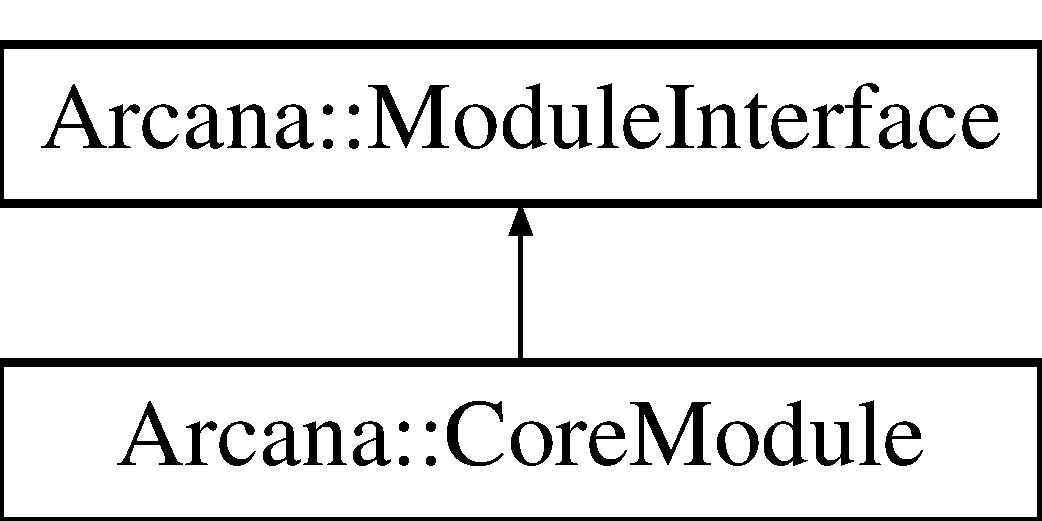
\includegraphics[height=2.000000cm]{class_arcana_1_1_module_interface}
\end{center}
\end{figure}
\subsection*{Public Member Functions}
\begin{DoxyCompactItemize}
\item 
\mbox{\Hypertarget{class_arcana_1_1_module_interface_a13db439f91f251753335e244d7199d10}\label{class_arcana_1_1_module_interface_a13db439f91f251753335e244d7199d10}} 
virtual \mbox{\hyperlink{class_arcana_1_1_module_interface_a13db439f91f251753335e244d7199d10}{$\sim$\+Module\+Interface}} ()
\begin{DoxyCompactList}\small\item\em \mbox{\hyperlink{class_arcana_1_1_module_interface}{Module\+Interface}} destructor. \end{DoxyCompactList}\item 
\mbox{\Hypertarget{class_arcana_1_1_module_interface_abc52ffd77b2adcea7128816587dd09ad}\label{class_arcana_1_1_module_interface_abc52ffd77b2adcea7128816587dd09ad}} 
virtual bool \mbox{\hyperlink{class_arcana_1_1_module_interface_abc52ffd77b2adcea7128816587dd09ad}{start\+Up}} ()=0
\begin{DoxyCompactList}\small\item\em Starts up the module. \end{DoxyCompactList}\item 
\mbox{\Hypertarget{class_arcana_1_1_module_interface_aca005760af4a5d2a32e5d3c79da61c4c}\label{class_arcana_1_1_module_interface_aca005760af4a5d2a32e5d3c79da61c4c}} 
virtual bool \mbox{\hyperlink{class_arcana_1_1_module_interface_aca005760af4a5d2a32e5d3c79da61c4c}{shut\+Down}} ()=0
\begin{DoxyCompactList}\small\item\em Shuts down the module. \end{DoxyCompactList}\item 
\mbox{\Hypertarget{class_arcana_1_1_module_interface_a2836a901809149b08e25a36a8e939a44}\label{class_arcana_1_1_module_interface_a2836a901809149b08e25a36a8e939a44}} 
virtual bool \mbox{\hyperlink{class_arcana_1_1_module_interface_a2836a901809149b08e25a36a8e939a44}{is\+Game\+Module}} ()=0
\begin{DoxyCompactList}\small\item\em Returns true if the module is game specific. \end{DoxyCompactList}\end{DoxyCompactItemize}


\subsection{Detailed Description}
Interface for Engine and Game modules. 

The documentation for this class was generated from the following file\+:\begin{DoxyCompactItemize}
\item 
Module\+Interface.\+h\end{DoxyCompactItemize}

\hypertarget{class_arcana_1_1_mouse_event}{}\section{Arcana\+:\+:Mouse\+Event Class Reference}
\label{class_arcana_1_1_mouse_event}\index{Arcana\+::\+Mouse\+Event@{Arcana\+::\+Mouse\+Event}}


\mbox{\hyperlink{class_arcana_1_1_event}{Event}} broadcasted on mouse presses/releases/movement/etc.  




{\ttfamily \#include $<$Mouse\+Event.\+h$>$}

Inheritance diagram for Arcana\+:\+:Mouse\+Event\+:\begin{figure}[H]
\begin{center}
\leavevmode
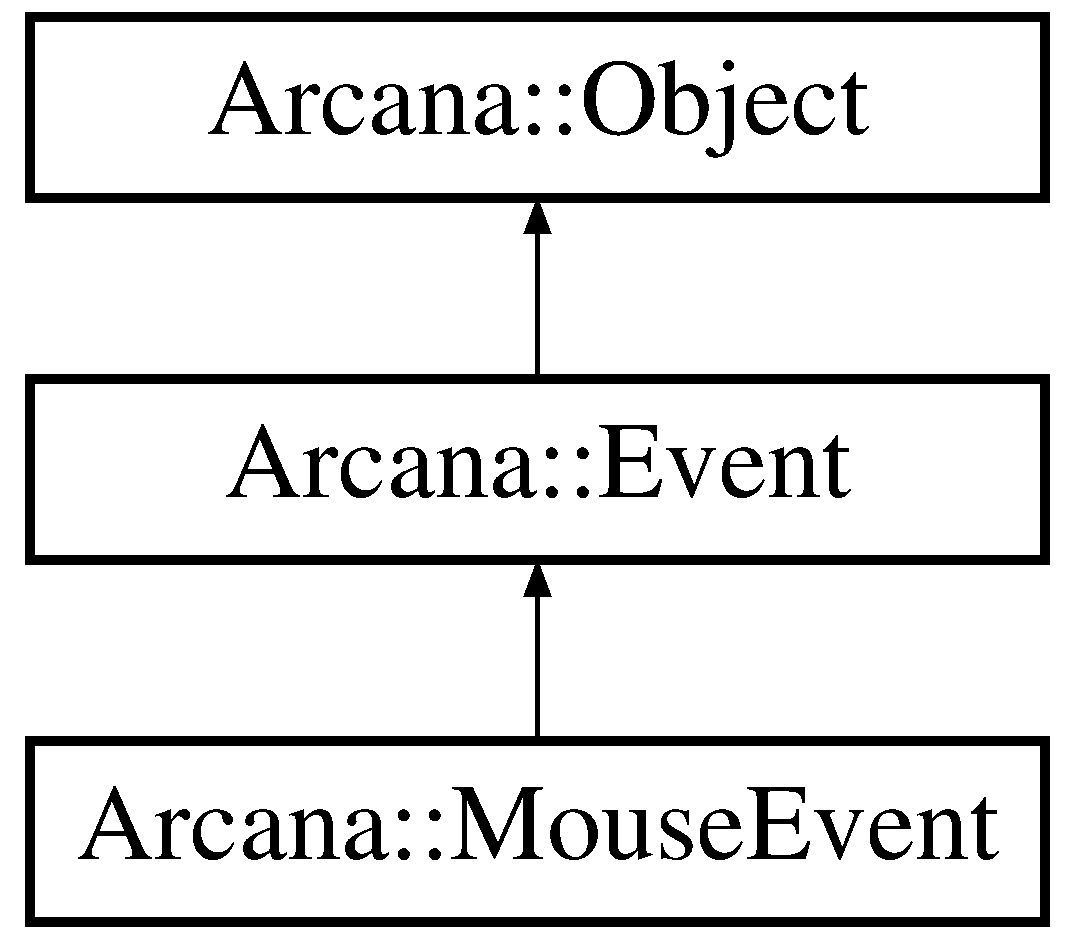
\includegraphics[height=3.000000cm]{class_arcana_1_1_mouse_event}
\end{center}
\end{figure}
\subsection*{Public Types}
\begin{DoxyCompactItemize}
\item 
enum \mbox{\hyperlink{class_arcana_1_1_mouse_event_aef6393d6d26e822bd527617c64acadea}{Type}} \{ \newline
\mbox{\hyperlink{class_arcana_1_1_mouse_event_aef6393d6d26e822bd527617c64acadeaa39ff2644effe01ad775b26b729c8c6fd}{Wheel\+Moved}}, 
\mbox{\hyperlink{class_arcana_1_1_mouse_event_aef6393d6d26e822bd527617c64acadeaad7163efce4b5c60707606f4905311c47}{Wheel\+Scrolled}}, 
\mbox{\hyperlink{class_arcana_1_1_mouse_event_aef6393d6d26e822bd527617c64acadeaa6b16a05bed85e41f056fdc640d6c637d}{Moved}}, 
\mbox{\hyperlink{class_arcana_1_1_mouse_event_aef6393d6d26e822bd527617c64acadeaa63a98f046ad0408b1b774f57e4eb659b}{Entered}}, 
\newline
\mbox{\hyperlink{class_arcana_1_1_mouse_event_aef6393d6d26e822bd527617c64acadeaae61245a192edadfee9347c2a524f689e}{Exited}}
 \}
\begin{DoxyCompactList}\small\item\em Mouse event type. \end{DoxyCompactList}\item 
enum \mbox{\hyperlink{class_arcana_1_1_mouse_event_aa658cf03c3ae261e9552804c0e0a46dd}{Wheel}} \{ \mbox{\hyperlink{class_arcana_1_1_mouse_event_aa658cf03c3ae261e9552804c0e0a46dda42b46757e2b876a14045d2ce8e4a5302}{Vertical}}, 
\mbox{\hyperlink{class_arcana_1_1_mouse_event_aa658cf03c3ae261e9552804c0e0a46dda5c63bd8a3472b3726d58675251036727}{Horizontal}}
 \}
\begin{DoxyCompactList}\small\item\em Mouse wheel ID. \end{DoxyCompactList}\end{DoxyCompactItemize}
\subsection*{Public Member Functions}
\begin{DoxyCompactItemize}
\item 
\mbox{\Hypertarget{class_arcana_1_1_mouse_event_a69650ca386ade5d366d05671c4be3780}\label{class_arcana_1_1_mouse_event_a69650ca386ade5d366d05671c4be3780}} 
\mbox{\hyperlink{class_arcana_1_1_mouse_event_a69650ca386ade5d366d05671c4be3780}{Mouse\+Event}} (\mbox{\hyperlink{class_arcana_1_1_mouse_event_aef6393d6d26e822bd527617c64acadea}{Type}} event, int x, int y, uint64 button)
\begin{DoxyCompactList}\small\item\em \mbox{\hyperlink{class_arcana_1_1_mouse_event}{Mouse\+Event}} button press constructor. \end{DoxyCompactList}\item 
\mbox{\Hypertarget{class_arcana_1_1_mouse_event_ad66da4ca5b708d640f5fc13b620b0d15}\label{class_arcana_1_1_mouse_event_ad66da4ca5b708d640f5fc13b620b0d15}} 
\mbox{\hyperlink{class_arcana_1_1_mouse_event_ad66da4ca5b708d640f5fc13b620b0d15}{Mouse\+Event}} (int x, int y, int delta)
\begin{DoxyCompactList}\small\item\em \mbox{\hyperlink{class_arcana_1_1_mouse_event}{Mouse\+Event}} wheel moved constructor. \end{DoxyCompactList}\item 
\mbox{\Hypertarget{class_arcana_1_1_mouse_event_af578af2045606d94736d2f59be861a37}\label{class_arcana_1_1_mouse_event_af578af2045606d94736d2f59be861a37}} 
\mbox{\hyperlink{class_arcana_1_1_mouse_event_af578af2045606d94736d2f59be861a37}{Mouse\+Event}} (int x, int y, float delta, \mbox{\hyperlink{class_arcana_1_1_mouse_event_aa658cf03c3ae261e9552804c0e0a46dd}{Wheel}} wheel)
\begin{DoxyCompactList}\small\item\em \mbox{\hyperlink{class_arcana_1_1_mouse_event}{Mouse\+Event}} wheel scrolled constructor. \end{DoxyCompactList}\item 
\mbox{\Hypertarget{class_arcana_1_1_mouse_event_ac249939756a1158fbe5897bf7760dfa4}\label{class_arcana_1_1_mouse_event_ac249939756a1158fbe5897bf7760dfa4}} 
\mbox{\hyperlink{class_arcana_1_1_mouse_event_ac249939756a1158fbe5897bf7760dfa4}{Mouse\+Event}} (int x, int y)
\begin{DoxyCompactList}\small\item\em \mbox{\hyperlink{class_arcana_1_1_mouse_event}{Mouse\+Event}} moved constructor. \end{DoxyCompactList}\item 
\mbox{\Hypertarget{class_arcana_1_1_mouse_event_a638a251a9da475e8ac418a1239b8c99d}\label{class_arcana_1_1_mouse_event_a638a251a9da475e8ac418a1239b8c99d}} 
\mbox{\hyperlink{class_arcana_1_1_mouse_event_a638a251a9da475e8ac418a1239b8c99d}{Mouse\+Event}} (\mbox{\hyperlink{class_arcana_1_1_mouse_event_aef6393d6d26e822bd527617c64acadea}{Type}} event)
\begin{DoxyCompactList}\small\item\em \mbox{\hyperlink{class_arcana_1_1_mouse_event}{Mouse\+Event}} constructor. \end{DoxyCompactList}\end{DoxyCompactItemize}


\subsection{Detailed Description}
\mbox{\hyperlink{class_arcana_1_1_event}{Event}} broadcasted on mouse presses/releases/movement/etc. 

Mouse\+Events have and event id of 2. 

\subsection{Member Enumeration Documentation}
\mbox{\Hypertarget{class_arcana_1_1_mouse_event_aef6393d6d26e822bd527617c64acadea}\label{class_arcana_1_1_mouse_event_aef6393d6d26e822bd527617c64acadea}} 
\index{Arcana\+::\+Mouse\+Event@{Arcana\+::\+Mouse\+Event}!Type@{Type}}
\index{Type@{Type}!Arcana\+::\+Mouse\+Event@{Arcana\+::\+Mouse\+Event}}
\subsubsection{\texorpdfstring{Type}{Type}}
{\footnotesize\ttfamily enum \mbox{\hyperlink{class_arcana_1_1_mouse_event_aef6393d6d26e822bd527617c64acadea}{Arcana\+::\+Mouse\+Event\+::\+Type}}}



Mouse event type. 

\begin{DoxyEnumFields}{Enumerator}
\raisebox{\heightof{T}}[0pt][0pt]{\index{Wheel\+Moved@{Wheel\+Moved}!Arcana\+::\+Mouse\+Event@{Arcana\+::\+Mouse\+Event}}\index{Arcana\+::\+Mouse\+Event@{Arcana\+::\+Mouse\+Event}!Wheel\+Moved@{Wheel\+Moved}}}\mbox{\Hypertarget{class_arcana_1_1_mouse_event_aef6393d6d26e822bd527617c64acadeaa39ff2644effe01ad775b26b729c8c6fd}\label{class_arcana_1_1_mouse_event_aef6393d6d26e822bd527617c64acadeaa39ff2644effe01ad775b26b729c8c6fd}} 
Wheel\+Moved&Mouse wheel moved. \\
\hline

\raisebox{\heightof{T}}[0pt][0pt]{\index{Wheel\+Scrolled@{Wheel\+Scrolled}!Arcana\+::\+Mouse\+Event@{Arcana\+::\+Mouse\+Event}}\index{Arcana\+::\+Mouse\+Event@{Arcana\+::\+Mouse\+Event}!Wheel\+Scrolled@{Wheel\+Scrolled}}}\mbox{\Hypertarget{class_arcana_1_1_mouse_event_aef6393d6d26e822bd527617c64acadeaad7163efce4b5c60707606f4905311c47}\label{class_arcana_1_1_mouse_event_aef6393d6d26e822bd527617c64acadeaad7163efce4b5c60707606f4905311c47}} 
Wheel\+Scrolled&Mouse wheel scrolled. \\
\hline

\raisebox{\heightof{T}}[0pt][0pt]{\index{Moved@{Moved}!Arcana\+::\+Mouse\+Event@{Arcana\+::\+Mouse\+Event}}\index{Arcana\+::\+Mouse\+Event@{Arcana\+::\+Mouse\+Event}!Moved@{Moved}}}\mbox{\Hypertarget{class_arcana_1_1_mouse_event_aef6393d6d26e822bd527617c64acadeaa6b16a05bed85e41f056fdc640d6c637d}\label{class_arcana_1_1_mouse_event_aef6393d6d26e822bd527617c64acadeaa6b16a05bed85e41f056fdc640d6c637d}} 
Moved&Mouse moved. \\
\hline

\raisebox{\heightof{T}}[0pt][0pt]{\index{Entered@{Entered}!Arcana\+::\+Mouse\+Event@{Arcana\+::\+Mouse\+Event}}\index{Arcana\+::\+Mouse\+Event@{Arcana\+::\+Mouse\+Event}!Entered@{Entered}}}\mbox{\Hypertarget{class_arcana_1_1_mouse_event_aef6393d6d26e822bd527617c64acadeaa63a98f046ad0408b1b774f57e4eb659b}\label{class_arcana_1_1_mouse_event_aef6393d6d26e822bd527617c64acadeaa63a98f046ad0408b1b774f57e4eb659b}} 
Entered&Mouse ented the window. \\
\hline

\raisebox{\heightof{T}}[0pt][0pt]{\index{Exited@{Exited}!Arcana\+::\+Mouse\+Event@{Arcana\+::\+Mouse\+Event}}\index{Arcana\+::\+Mouse\+Event@{Arcana\+::\+Mouse\+Event}!Exited@{Exited}}}\mbox{\Hypertarget{class_arcana_1_1_mouse_event_aef6393d6d26e822bd527617c64acadeaae61245a192edadfee9347c2a524f689e}\label{class_arcana_1_1_mouse_event_aef6393d6d26e822bd527617c64acadeaae61245a192edadfee9347c2a524f689e}} 
Exited&Mouse ented the exited. \\
\hline

\end{DoxyEnumFields}
\mbox{\Hypertarget{class_arcana_1_1_mouse_event_aa658cf03c3ae261e9552804c0e0a46dd}\label{class_arcana_1_1_mouse_event_aa658cf03c3ae261e9552804c0e0a46dd}} 
\index{Arcana\+::\+Mouse\+Event@{Arcana\+::\+Mouse\+Event}!Wheel@{Wheel}}
\index{Wheel@{Wheel}!Arcana\+::\+Mouse\+Event@{Arcana\+::\+Mouse\+Event}}
\subsubsection{\texorpdfstring{Wheel}{Wheel}}
{\footnotesize\ttfamily enum \mbox{\hyperlink{class_arcana_1_1_mouse_event_aa658cf03c3ae261e9552804c0e0a46dd}{Arcana\+::\+Mouse\+Event\+::\+Wheel}}}



Mouse wheel ID. 

\begin{DoxyEnumFields}{Enumerator}
\raisebox{\heightof{T}}[0pt][0pt]{\index{Vertical@{Vertical}!Arcana\+::\+Mouse\+Event@{Arcana\+::\+Mouse\+Event}}\index{Arcana\+::\+Mouse\+Event@{Arcana\+::\+Mouse\+Event}!Vertical@{Vertical}}}\mbox{\Hypertarget{class_arcana_1_1_mouse_event_aa658cf03c3ae261e9552804c0e0a46dda42b46757e2b876a14045d2ce8e4a5302}\label{class_arcana_1_1_mouse_event_aa658cf03c3ae261e9552804c0e0a46dda42b46757e2b876a14045d2ce8e4a5302}} 
Vertical&Vertical wheel. \\
\hline

\raisebox{\heightof{T}}[0pt][0pt]{\index{Horizontal@{Horizontal}!Arcana\+::\+Mouse\+Event@{Arcana\+::\+Mouse\+Event}}\index{Arcana\+::\+Mouse\+Event@{Arcana\+::\+Mouse\+Event}!Horizontal@{Horizontal}}}\mbox{\Hypertarget{class_arcana_1_1_mouse_event_aa658cf03c3ae261e9552804c0e0a46dda5c63bd8a3472b3726d58675251036727}\label{class_arcana_1_1_mouse_event_aa658cf03c3ae261e9552804c0e0a46dda5c63bd8a3472b3726d58675251036727}} 
Horizontal&Horizontal wheel. \\
\hline

\end{DoxyEnumFields}


The documentation for this class was generated from the following file\+:\begin{DoxyCompactItemize}
\item 
Mouse\+Event.\+h\end{DoxyCompactItemize}

\hypertarget{class_arcana_1_1_object}{}\section{Arcana\+:\+:Object Class Reference}
\label{class_arcana_1_1_object}\index{Arcana\+::\+Object@{Arcana\+::\+Object}}


The base class for all core classes.  




{\ttfamily \#include $<$Object.\+h$>$}

Inheritance diagram for Arcana\+:\+:Object\+:\begin{figure}[H]
\begin{center}
\leavevmode
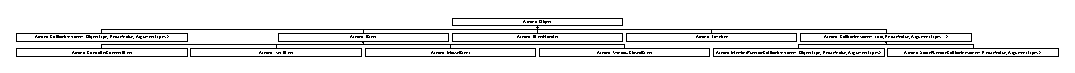
\includegraphics[height=0.534351cm]{class_arcana_1_1_object}
\end{center}
\end{figure}
\subsection*{Public Member Functions}
\begin{DoxyCompactItemize}
\item 
\mbox{\Hypertarget{class_arcana_1_1_object_acb1521e4c8580906e56728d16b24c6e5}\label{class_arcana_1_1_object_acb1521e4c8580906e56728d16b24c6e5}} 
\mbox{\hyperlink{class_arcana_1_1_object_acb1521e4c8580906e56728d16b24c6e5}{Object}} ()
\begin{DoxyCompactList}\small\item\em \mbox{\hyperlink{class_arcana_1_1_object}{Object}} default constructor. \end{DoxyCompactList}\item 
\mbox{\Hypertarget{class_arcana_1_1_object_a9b9a5d995e9a713adb3b301a3882aa60}\label{class_arcana_1_1_object_a9b9a5d995e9a713adb3b301a3882aa60}} 
\mbox{\hyperlink{class_arcana_1_1_object_a9b9a5d995e9a713adb3b301a3882aa60}{Object}} (const std\+::string \&type)
\begin{DoxyCompactList}\small\item\em \mbox{\hyperlink{class_arcana_1_1_object}{Object}} constructor with type argument. \end{DoxyCompactList}\item 
\mbox{\Hypertarget{class_arcana_1_1_object_a0f38ca8789a77c3bca2f70d19a9fcdf0}\label{class_arcana_1_1_object_a0f38ca8789a77c3bca2f70d19a9fcdf0}} 
\mbox{\hyperlink{class_arcana_1_1_object_a0f38ca8789a77c3bca2f70d19a9fcdf0}{Object}} (const \mbox{\hyperlink{class_arcana_1_1_object}{Object}} \&object)
\begin{DoxyCompactList}\small\item\em \mbox{\hyperlink{class_arcana_1_1_object}{Object}} copy constructor. \end{DoxyCompactList}\item 
\mbox{\Hypertarget{class_arcana_1_1_object_afa6ae7570a5abb7938af786a15154046}\label{class_arcana_1_1_object_afa6ae7570a5abb7938af786a15154046}} 
virtual \mbox{\hyperlink{class_arcana_1_1_object_afa6ae7570a5abb7938af786a15154046}{$\sim$\+Object}} ()
\begin{DoxyCompactList}\small\item\em \mbox{\hyperlink{class_arcana_1_1_object}{Object}} destructor (should be virtual?) \end{DoxyCompactList}\item 
\mbox{\Hypertarget{class_arcana_1_1_object_a2de0f40152fa8b1914a6449456757a24}\label{class_arcana_1_1_object_a2de0f40152fa8b1914a6449456757a24}} 
const std\+::string \& \mbox{\hyperlink{class_arcana_1_1_object_a2de0f40152fa8b1914a6449456757a24}{get\+Type}} () const
\begin{DoxyCompactList}\small\item\em Accessor for the object type. \end{DoxyCompactList}\item 
\mbox{\Hypertarget{class_arcana_1_1_object_a8851a34872b31b360d4e574d2d47ba67}\label{class_arcana_1_1_object_a8851a34872b31b360d4e574d2d47ba67}} 
void $\ast$ \mbox{\hyperlink{class_arcana_1_1_object_a8851a34872b31b360d4e574d2d47ba67}{get\+User\+Data}} () const
\begin{DoxyCompactList}\small\item\em Accessor for the object\textquotesingle{}s user data. \end{DoxyCompactList}\item 
\mbox{\Hypertarget{class_arcana_1_1_object_a34092d7ea25f17823e6ccf1e6e110152}\label{class_arcana_1_1_object_a34092d7ea25f17823e6ccf1e6e110152}} 
void \mbox{\hyperlink{class_arcana_1_1_object_a34092d7ea25f17823e6ccf1e6e110152}{set\+User\+Data}} (void $\ast$data)
\begin{DoxyCompactList}\small\item\em Mutator for the object\textquotesingle{}s user data. \end{DoxyCompactList}\item 
virtual int32 \mbox{\hyperlink{class_arcana_1_1_object_aee21c11c6df1f204288c55cab27139fe}{reference}} ()
\begin{DoxyCompactList}\small\item\em Increments the reference count. \end{DoxyCompactList}\item 
virtual void \mbox{\hyperlink{class_arcana_1_1_object_aa14c503a92c2a630c119c5a21ea040f8}{release}} ()
\begin{DoxyCompactList}\small\item\em Decrements the reference count. \end{DoxyCompactList}\item 
virtual int32 \mbox{\hyperlink{class_arcana_1_1_object_ae9a43cf92c71ea1e5a672b40e9a99f19}{reference\+Count}} ()
\begin{DoxyCompactList}\small\item\em Increments the reference count. \end{DoxyCompactList}\item 
\mbox{\Hypertarget{class_arcana_1_1_object_af08a90d6cc61992f2908e61b60a31972}\label{class_arcana_1_1_object_af08a90d6cc61992f2908e61b60a31972}} 
void \mbox{\hyperlink{class_arcana_1_1_object_af08a90d6cc61992f2908e61b60a31972}{mark\+For\+Destruction}} ()
\begin{DoxyCompactList}\small\item\em Marks the object to be destroyed by the garbage collector. \end{DoxyCompactList}\item 
\mbox{\Hypertarget{class_arcana_1_1_object_aa885d48e135268cc4198ccb550e151aa}\label{class_arcana_1_1_object_aa885d48e135268cc4198ccb550e151aa}} 
bool \mbox{\hyperlink{class_arcana_1_1_object_aa885d48e135268cc4198ccb550e151aa}{is\+Pending\+Destroy}} () const
\begin{DoxyCompactList}\small\item\em Returns true if the object has been marked for destruction. \end{DoxyCompactList}\item 
void \mbox{\hyperlink{class_arcana_1_1_object_abd84158043b5d90a1f1c5647c0f04b9f}{allow\+Destruction}} ()
\begin{DoxyCompactList}\small\item\em Allows the garbage collector to destroyed the object. \end{DoxyCompactList}\item 
\mbox{\Hypertarget{class_arcana_1_1_object_a2cbe52bfff3d3c70e35a5de48d7081d4}\label{class_arcana_1_1_object_a2cbe52bfff3d3c70e35a5de48d7081d4}} 
bool \mbox{\hyperlink{class_arcana_1_1_object_a2cbe52bfff3d3c70e35a5de48d7081d4}{can\+Be\+Destroyed}} () const
\begin{DoxyCompactList}\small\item\em Returns true if the object can be destroyed. \end{DoxyCompactList}\item 
\mbox{\Hypertarget{class_arcana_1_1_object_acd005d9de1a1e009b9851901fd678ac3}\label{class_arcana_1_1_object_acd005d9de1a1e009b9851901fd678ac3}} 
\mbox{\hyperlink{class_arcana_1_1_object}{Object}} \& \mbox{\hyperlink{class_arcana_1_1_object_acd005d9de1a1e009b9851901fd678ac3}{operator=}} (const \mbox{\hyperlink{class_arcana_1_1_object}{Object}} \&object)
\begin{DoxyCompactList}\small\item\em \mbox{\hyperlink{class_arcana_1_1_object}{Object}} assignment operator. \end{DoxyCompactList}\end{DoxyCompactItemize}


\subsection{Detailed Description}
The base class for all core classes. 



\subsection{Member Function Documentation}
\mbox{\Hypertarget{class_arcana_1_1_object_abd84158043b5d90a1f1c5647c0f04b9f}\label{class_arcana_1_1_object_abd84158043b5d90a1f1c5647c0f04b9f}} 
\index{Arcana\+::\+Object@{Arcana\+::\+Object}!allow\+Destruction@{allow\+Destruction}}
\index{allow\+Destruction@{allow\+Destruction}!Arcana\+::\+Object@{Arcana\+::\+Object}}
\subsubsection{\texorpdfstring{allow\+Destruction()}{allowDestruction()}}
{\footnotesize\ttfamily void Arcana\+::\+Object\+::allow\+Destruction (\begin{DoxyParamCaption}{ }\end{DoxyParamCaption})}



Allows the garbage collector to destroyed the object. 

Only works for objects that are marked for destruction. \mbox{\Hypertarget{class_arcana_1_1_object_aee21c11c6df1f204288c55cab27139fe}\label{class_arcana_1_1_object_aee21c11c6df1f204288c55cab27139fe}} 
\index{Arcana\+::\+Object@{Arcana\+::\+Object}!reference@{reference}}
\index{reference@{reference}!Arcana\+::\+Object@{Arcana\+::\+Object}}
\subsubsection{\texorpdfstring{reference()}{reference()}}
{\footnotesize\ttfamily int32 Arcana\+::\+Object\+::reference (\begin{DoxyParamCaption}{ }\end{DoxyParamCaption})\hspace{0.3cm}{\ttfamily [virtual]}}



Increments the reference count. 

Returns the current reference count. \mbox{\Hypertarget{class_arcana_1_1_object_ae9a43cf92c71ea1e5a672b40e9a99f19}\label{class_arcana_1_1_object_ae9a43cf92c71ea1e5a672b40e9a99f19}} 
\index{Arcana\+::\+Object@{Arcana\+::\+Object}!reference\+Count@{reference\+Count}}
\index{reference\+Count@{reference\+Count}!Arcana\+::\+Object@{Arcana\+::\+Object}}
\subsubsection{\texorpdfstring{reference\+Count()}{referenceCount()}}
{\footnotesize\ttfamily int32 Arcana\+::\+Object\+::reference\+Count (\begin{DoxyParamCaption}{ }\end{DoxyParamCaption})\hspace{0.3cm}{\ttfamily [virtual]}}



Increments the reference count. 

Returns the current reference count. \mbox{\Hypertarget{class_arcana_1_1_object_aa14c503a92c2a630c119c5a21ea040f8}\label{class_arcana_1_1_object_aa14c503a92c2a630c119c5a21ea040f8}} 
\index{Arcana\+::\+Object@{Arcana\+::\+Object}!release@{release}}
\index{release@{release}!Arcana\+::\+Object@{Arcana\+::\+Object}}
\subsubsection{\texorpdfstring{release()}{release()}}
{\footnotesize\ttfamily void Arcana\+::\+Object\+::release (\begin{DoxyParamCaption}{ }\end{DoxyParamCaption})\hspace{0.3cm}{\ttfamily [virtual]}}



Decrements the reference count. 

Deletes the object if the reference count is zero. 

The documentation for this class was generated from the following files\+:\begin{DoxyCompactItemize}
\item 
Object.\+h\item 
Object.\+cpp\end{DoxyCompactItemize}

\hypertarget{class_arcana_1_1_object_destruction_manager}{}\section{Arcana\+:\+:Object\+Destruction\+Manager Class Reference}
\label{class_arcana_1_1_object_destruction_manager}\index{Arcana\+::\+Object\+Destruction\+Manager@{Arcana\+::\+Object\+Destruction\+Manager}}


Manages automatic garbage collection.  




{\ttfamily \#include $<$Object\+Destruction\+Manager.\+h$>$}

\subsection*{Public Member Functions}
\begin{DoxyCompactItemize}
\item 
\mbox{\Hypertarget{class_arcana_1_1_object_destruction_manager_a21b58f25c4f9c8e567c95e719d3eabcd}\label{class_arcana_1_1_object_destruction_manager_a21b58f25c4f9c8e567c95e719d3eabcd}} 
\mbox{\hyperlink{class_arcana_1_1_object_destruction_manager_a21b58f25c4f9c8e567c95e719d3eabcd}{Object\+Destruction\+Manager}} ()
\begin{DoxyCompactList}\small\item\em \mbox{\hyperlink{class_arcana_1_1_object_destruction_manager}{Object\+Destruction\+Manager}} default constructor. \end{DoxyCompactList}\item 
\mbox{\Hypertarget{class_arcana_1_1_object_destruction_manager_a96f677144d9eb0d4ecf64d6f20735f59}\label{class_arcana_1_1_object_destruction_manager_a96f677144d9eb0d4ecf64d6f20735f59}} 
\mbox{\hyperlink{class_arcana_1_1_object_destruction_manager_a96f677144d9eb0d4ecf64d6f20735f59}{$\sim$\+Object\+Destruction\+Manager}} ()
\begin{DoxyCompactList}\small\item\em \mbox{\hyperlink{class_arcana_1_1_object_destruction_manager}{Object\+Destruction\+Manager}} destructor. \end{DoxyCompactList}\item 
\mbox{\Hypertarget{class_arcana_1_1_object_destruction_manager_a0ae07d47fe0930b39d92a4b2da16b1c1}\label{class_arcana_1_1_object_destruction_manager_a0ae07d47fe0930b39d92a4b2da16b1c1}} 
void \mbox{\hyperlink{class_arcana_1_1_object_destruction_manager_a0ae07d47fe0930b39d92a4b2da16b1c1}{add\+Pending\+Cleanup\+Object}} (\mbox{\hyperlink{class_arcana_1_1_object}{Object}} $\ast$object)
\begin{DoxyCompactList}\small\item\em Adds an \mbox{\hyperlink{class_arcana_1_1_object}{Object}} to the pending cleanup queue. \end{DoxyCompactList}\item 
void \mbox{\hyperlink{class_arcana_1_1_object_destruction_manager_a662cd206b7da25f1f25d7aeab978740d}{cleanup\+Objects}} ()
\begin{DoxyCompactList}\small\item\em Cleans up any objects that can be destroyed. \end{DoxyCompactList}\end{DoxyCompactItemize}
\subsection*{Static Public Member Functions}
\begin{DoxyCompactItemize}
\item 
\mbox{\Hypertarget{class_arcana_1_1_object_destruction_manager_a53d504581d3835324bb5fe5b5d487401}\label{class_arcana_1_1_object_destruction_manager_a53d504581d3835324bb5fe5b5d487401}} 
static \mbox{\hyperlink{class_arcana_1_1_object_destruction_manager}{Object\+Destruction\+Manager}} \& \mbox{\hyperlink{class_arcana_1_1_object_destruction_manager_a53d504581d3835324bb5fe5b5d487401}{instance}} ()
\begin{DoxyCompactList}\small\item\em Singleton instance accessor. \end{DoxyCompactList}\end{DoxyCompactItemize}


\subsection{Detailed Description}
Manages automatic garbage collection. 

\subsection{Member Function Documentation}
\mbox{\Hypertarget{class_arcana_1_1_object_destruction_manager_a662cd206b7da25f1f25d7aeab978740d}\label{class_arcana_1_1_object_destruction_manager_a662cd206b7da25f1f25d7aeab978740d}} 
\index{Arcana\+::\+Object\+Destruction\+Manager@{Arcana\+::\+Object\+Destruction\+Manager}!cleanup\+Objects@{cleanup\+Objects}}
\index{cleanup\+Objects@{cleanup\+Objects}!Arcana\+::\+Object\+Destruction\+Manager@{Arcana\+::\+Object\+Destruction\+Manager}}
\subsubsection{\texorpdfstring{cleanup\+Objects()}{cleanupObjects()}}
{\footnotesize\ttfamily void Arcana\+::\+Object\+Destruction\+Manager\+::cleanup\+Objects (\begin{DoxyParamCaption}{ }\end{DoxyParamCaption})}



Cleans up any objects that can be destroyed. 

Called every update cycle by the main engine loop. 

The documentation for this class was generated from the following files\+:\begin{DoxyCompactItemize}
\item 
Object\+Destruction\+Manager.\+h\item 
Object\+Destruction\+Manager.\+cpp\end{DoxyCompactItemize}

\hypertarget{class_arcana_1_1_profile_manager}{}\section{Arcana\+:\+:Profile\+Manager Class Reference}
\label{class_arcana_1_1_profile_manager}\index{Arcana\+::\+Profile\+Manager@{Arcana\+::\+Profile\+Manager}}


Manager for profile samples.  




{\ttfamily \#include $<$Profile\+Manager.\+h$>$}

\subsection*{Public Member Functions}
\begin{DoxyCompactItemize}
\item 
\mbox{\Hypertarget{class_arcana_1_1_profile_manager_a4a65e6962c23f6d40f905d89c6850805}\label{class_arcana_1_1_profile_manager_a4a65e6962c23f6d40f905d89c6850805}} 
void \mbox{\hyperlink{class_arcana_1_1_profile_manager_a4a65e6962c23f6d40f905d89c6850805}{export\+Samples}} (const std\+::string \&output\+File)
\begin{DoxyCompactList}\small\item\em Exports the samples to a csv file. \end{DoxyCompactList}\item 
\mbox{\Hypertarget{class_arcana_1_1_profile_manager_a9b4e75f1ce6aae83bd06479a6c4efc3a}\label{class_arcana_1_1_profile_manager_a9b4e75f1ce6aae83bd06479a6c4efc3a}} 
void \mbox{\hyperlink{class_arcana_1_1_profile_manager_a9b4e75f1ce6aae83bd06479a6c4efc3a}{store\+Sample}} (const char $\ast$name, int64 elapsed\+Time)
\begin{DoxyCompactList}\small\item\em Stores a profile sample. \end{DoxyCompactList}\end{DoxyCompactItemize}
\subsection*{Static Public Member Functions}
\begin{DoxyCompactItemize}
\item 
\mbox{\Hypertarget{class_arcana_1_1_profile_manager_aca7041e5f3e4b33258f73f2138b8fbd4}\label{class_arcana_1_1_profile_manager_aca7041e5f3e4b33258f73f2138b8fbd4}} 
static \mbox{\hyperlink{class_arcana_1_1_profile_manager}{Profile\+Manager}} \& \mbox{\hyperlink{class_arcana_1_1_profile_manager_aca7041e5f3e4b33258f73f2138b8fbd4}{instance}} ()
\begin{DoxyCompactList}\small\item\em Singleton instance accessor. \end{DoxyCompactList}\end{DoxyCompactItemize}


\subsection{Detailed Description}
Manager for profile samples. 

Stores profile samples and exports a csv. 

The documentation for this class was generated from the following files\+:\begin{DoxyCompactItemize}
\item 
Profile\+Manager.\+h\item 
Profile\+Manager.\+cpp\end{DoxyCompactItemize}

\hypertarget{struct_arcana_1_1_remove_reference}{}\section{Arcana\+:\+:Remove\+Reference$<$ T $>$ Struct Template Reference}
\label{struct_arcana_1_1_remove_reference}\index{Arcana\+::\+Remove\+Reference$<$ T $>$@{Arcana\+::\+Remove\+Reference$<$ T $>$}}
\subsection*{Public Types}
\begin{DoxyCompactItemize}
\item 
\mbox{\Hypertarget{struct_arcana_1_1_remove_reference_a906acbdca72d0c56e200b55fe0217a32}\label{struct_arcana_1_1_remove_reference_a906acbdca72d0c56e200b55fe0217a32}} 
typedef T {\bfseries Type}
\end{DoxyCompactItemize}


The documentation for this struct was generated from the following file\+:\begin{DoxyCompactItemize}
\item 
Arcana\+Template.\+h\end{DoxyCompactItemize}

\hypertarget{struct_arcana_1_1_remove_reference_3_01_t_01_6_6_01_4}{}\section{Arcana\+:\+:Remove\+Reference$<$ T \&\& $>$ Struct Template Reference}
\label{struct_arcana_1_1_remove_reference_3_01_t_01_6_6_01_4}\index{Arcana\+::\+Remove\+Reference$<$ T \&\& $>$@{Arcana\+::\+Remove\+Reference$<$ T \&\& $>$}}
\subsection*{Public Types}
\begin{DoxyCompactItemize}
\item 
\mbox{\Hypertarget{struct_arcana_1_1_remove_reference_3_01_t_01_6_6_01_4_a5725b23062432b709ad14906725d3f79}\label{struct_arcana_1_1_remove_reference_3_01_t_01_6_6_01_4_a5725b23062432b709ad14906725d3f79}} 
typedef T {\bfseries Type}
\end{DoxyCompactItemize}


The documentation for this struct was generated from the following file\+:\begin{DoxyCompactItemize}
\item 
Arcana\+Template.\+h\end{DoxyCompactItemize}

\hypertarget{struct_arcana_1_1_remove_reference_3_01_t_01_6_4}{}\section{Arcana\+:\+:Remove\+Reference$<$ T \&$>$ Struct Template Reference}
\label{struct_arcana_1_1_remove_reference_3_01_t_01_6_4}\index{Arcana\+::\+Remove\+Reference$<$ T \&$>$@{Arcana\+::\+Remove\+Reference$<$ T \&$>$}}
\subsection*{Public Types}
\begin{DoxyCompactItemize}
\item 
\mbox{\Hypertarget{struct_arcana_1_1_remove_reference_3_01_t_01_6_4_a8f3f4fdb2bad28897a891085ebbcfdee}\label{struct_arcana_1_1_remove_reference_3_01_t_01_6_4_a8f3f4fdb2bad28897a891085ebbcfdee}} 
typedef T {\bfseries Type}
\end{DoxyCompactItemize}


The documentation for this struct was generated from the following file\+:\begin{DoxyCompactItemize}
\item 
Arcana\+Template.\+h\end{DoxyCompactItemize}

\hypertarget{class_arcana_1_1_sleep}{}\section{Arcana\+:\+:Sleep Class Reference}
\label{class_arcana_1_1_sleep}\index{Arcana\+::\+Sleep@{Arcana\+::\+Sleep}}


Platform-\/independent sleep implementation.  




{\ttfamily \#include $<$Sleep.\+h$>$}

\subsection*{Public Member Functions}
\begin{DoxyCompactItemize}
\item 
\mbox{\hyperlink{class_arcana_1_1_sleep_a27eb99f8568acc83c7bcc86cbc710ba7}{Sleep}} (\mbox{\hyperlink{class_arcana_1_1_time}{Time}} time)
\begin{DoxyCompactList}\small\item\em \mbox{\hyperlink{class_arcana_1_1_sleep}{Sleep}} constructor. \end{DoxyCompactList}\item 
\mbox{\hyperlink{class_arcana_1_1_sleep_a5fc0c3cb0108e59f517a6ec13eb2d9e5}{Sleep}} (int64 microseconds)
\begin{DoxyCompactList}\small\item\em \mbox{\hyperlink{class_arcana_1_1_sleep}{Sleep}} constructor. \end{DoxyCompactList}\item 
\mbox{\hyperlink{class_arcana_1_1_sleep_aa483019d78bd041cddda7b781671b971}{Sleep}} (double seconds)
\begin{DoxyCompactList}\small\item\em \mbox{\hyperlink{class_arcana_1_1_sleep}{Sleep}} constructor. \end{DoxyCompactList}\end{DoxyCompactItemize}


\subsection{Detailed Description}
Platform-\/independent sleep implementation. 

\subsection{Constructor \& Destructor Documentation}
\mbox{\Hypertarget{class_arcana_1_1_sleep_a27eb99f8568acc83c7bcc86cbc710ba7}\label{class_arcana_1_1_sleep_a27eb99f8568acc83c7bcc86cbc710ba7}} 
\index{Arcana\+::\+Sleep@{Arcana\+::\+Sleep}!Sleep@{Sleep}}
\index{Sleep@{Sleep}!Arcana\+::\+Sleep@{Arcana\+::\+Sleep}}
\subsubsection{\texorpdfstring{Sleep()}{Sleep()}\hspace{0.1cm}{\footnotesize\ttfamily [1/3]}}
{\footnotesize\ttfamily Arcana\+::\+Sleep\+::\+Sleep (\begin{DoxyParamCaption}\item[{\mbox{\hyperlink{class_arcana_1_1_time}{Time}}}]{time }\end{DoxyParamCaption})}



\mbox{\hyperlink{class_arcana_1_1_sleep}{Sleep}} constructor. 

Takes a \mbox{\hyperlink{class_arcana_1_1_time}{Time}} object as an argument. \mbox{\Hypertarget{class_arcana_1_1_sleep_a5fc0c3cb0108e59f517a6ec13eb2d9e5}\label{class_arcana_1_1_sleep_a5fc0c3cb0108e59f517a6ec13eb2d9e5}} 
\index{Arcana\+::\+Sleep@{Arcana\+::\+Sleep}!Sleep@{Sleep}}
\index{Sleep@{Sleep}!Arcana\+::\+Sleep@{Arcana\+::\+Sleep}}
\subsubsection{\texorpdfstring{Sleep()}{Sleep()}\hspace{0.1cm}{\footnotesize\ttfamily [2/3]}}
{\footnotesize\ttfamily Arcana\+::\+Sleep\+::\+Sleep (\begin{DoxyParamCaption}\item[{int64}]{microseconds }\end{DoxyParamCaption})}



\mbox{\hyperlink{class_arcana_1_1_sleep}{Sleep}} constructor. 

Takes a time in microseconds as an argument. \mbox{\Hypertarget{class_arcana_1_1_sleep_aa483019d78bd041cddda7b781671b971}\label{class_arcana_1_1_sleep_aa483019d78bd041cddda7b781671b971}} 
\index{Arcana\+::\+Sleep@{Arcana\+::\+Sleep}!Sleep@{Sleep}}
\index{Sleep@{Sleep}!Arcana\+::\+Sleep@{Arcana\+::\+Sleep}}
\subsubsection{\texorpdfstring{Sleep()}{Sleep()}\hspace{0.1cm}{\footnotesize\ttfamily [3/3]}}
{\footnotesize\ttfamily Arcana\+::\+Sleep\+::\+Sleep (\begin{DoxyParamCaption}\item[{double}]{seconds }\end{DoxyParamCaption})}



\mbox{\hyperlink{class_arcana_1_1_sleep}{Sleep}} constructor. 

Takes a time in seconds as an argument. 

The documentation for this class was generated from the following files\+:\begin{DoxyCompactItemize}
\item 
Sleep.\+h\item 
Sleep.\+cpp\end{DoxyCompactItemize}

\hypertarget{class_arcana_1_1_sleep_context}{}\section{Arcana\+:\+:Sleep\+Context Class Reference}
\label{class_arcana_1_1_sleep_context}\index{Arcana\+::\+Sleep\+Context@{Arcana\+::\+Sleep\+Context}}


Windows sleep implementation.  




{\ttfamily \#include $<$Windows\+Sleep\+Context.\+h$>$}

\subsection*{Static Public Member Functions}
\begin{DoxyCompactItemize}
\item 
\mbox{\Hypertarget{class_arcana_1_1_sleep_context_ab1d1ffcdeed934cdf248ba60e80dbe23}\label{class_arcana_1_1_sleep_context_ab1d1ffcdeed934cdf248ba60e80dbe23}} 
static void \mbox{\hyperlink{class_arcana_1_1_sleep_context_ab1d1ffcdeed934cdf248ba60e80dbe23}{sleep}} (\mbox{\hyperlink{class_arcana_1_1_time}{Time}} time)
\begin{DoxyCompactList}\small\item\em Sleeps for \textquotesingle{}time\textquotesingle{}. \end{DoxyCompactList}\end{DoxyCompactItemize}


\subsection{Detailed Description}
Windows sleep implementation. 

The documentation for this class was generated from the following files\+:\begin{DoxyCompactItemize}
\item 
Windows\+Sleep\+Context.\+h\item 
Windows\+Sleep\+Context.\+cpp\end{DoxyCompactItemize}

\hypertarget{class_arcana_1_1_smart_ptr}{}\section{Arcana\+:\+:Smart\+Ptr$<$ Object\+Type $>$ Class Template Reference}
\label{class_arcana_1_1_smart_ptr}\index{Arcana\+::\+Smart\+Ptr$<$ Object\+Type $>$@{Arcana\+::\+Smart\+Ptr$<$ Object\+Type $>$}}


A templated smart pointer implementation.  




{\ttfamily \#include $<$Smart\+Ptr.\+h$>$}

\subsection*{Public Member Functions}
\begin{DoxyCompactItemize}
\item 
\mbox{\Hypertarget{class_arcana_1_1_smart_ptr_ac5402f3afb6aaec3488ce68dfc3cef90}\label{class_arcana_1_1_smart_ptr_ac5402f3afb6aaec3488ce68dfc3cef90}} 
\mbox{\hyperlink{class_arcana_1_1_smart_ptr_ac5402f3afb6aaec3488ce68dfc3cef90}{Smart\+Ptr}} ()
\begin{DoxyCompactList}\small\item\em \mbox{\hyperlink{class_arcana_1_1_smart_ptr}{Smart\+Ptr}} default constructor. \end{DoxyCompactList}\item 
\mbox{\Hypertarget{class_arcana_1_1_smart_ptr_a0b767e277796018d3c670bc4cd4339f6}\label{class_arcana_1_1_smart_ptr_a0b767e277796018d3c670bc4cd4339f6}} 
\mbox{\hyperlink{class_arcana_1_1_smart_ptr_a0b767e277796018d3c670bc4cd4339f6}{Smart\+Ptr}} (Object\+Type $\ast$pointer)
\begin{DoxyCompactList}\small\item\em \mbox{\hyperlink{class_arcana_1_1_smart_ptr}{Smart\+Ptr}} constructor with raw pointer argument. \end{DoxyCompactList}\item 
\mbox{\Hypertarget{class_arcana_1_1_smart_ptr_ae43a5c6b6a9ad9b796fdc65a9b514dea}\label{class_arcana_1_1_smart_ptr_ae43a5c6b6a9ad9b796fdc65a9b514dea}} 
\mbox{\hyperlink{class_arcana_1_1_smart_ptr_ae43a5c6b6a9ad9b796fdc65a9b514dea}{Smart\+Ptr}} (const \mbox{\hyperlink{class_arcana_1_1_smart_ptr}{Smart\+Ptr}}$<$ Object\+Type $>$ \&ptr)
\begin{DoxyCompactList}\small\item\em \mbox{\hyperlink{class_arcana_1_1_smart_ptr}{Smart\+Ptr}} copy constructor. \end{DoxyCompactList}\item 
\mbox{\Hypertarget{class_arcana_1_1_smart_ptr_a045e89c8708a1c59cd796bf067aedeb9}\label{class_arcana_1_1_smart_ptr_a045e89c8708a1c59cd796bf067aedeb9}} 
\mbox{\hyperlink{class_arcana_1_1_smart_ptr_a045e89c8708a1c59cd796bf067aedeb9}{$\sim$\+Smart\+Ptr}} ()
\begin{DoxyCompactList}\small\item\em \mbox{\hyperlink{class_arcana_1_1_smart_ptr}{Smart\+Ptr}} destructor. \end{DoxyCompactList}\item 
\mbox{\Hypertarget{class_arcana_1_1_smart_ptr_ac030bd8f3d58c7a68fb95dcb9706f200}\label{class_arcana_1_1_smart_ptr_ac030bd8f3d58c7a68fb95dcb9706f200}} 
void \mbox{\hyperlink{class_arcana_1_1_smart_ptr_ac030bd8f3d58c7a68fb95dcb9706f200}{Add\+Reference}} ()
\begin{DoxyCompactList}\small\item\em Increments the reference counter. \end{DoxyCompactList}\item 
\mbox{\Hypertarget{class_arcana_1_1_smart_ptr_a285a88806044e2511cff05d518155d44}\label{class_arcana_1_1_smart_ptr_a285a88806044e2511cff05d518155d44}} 
unsigned int \mbox{\hyperlink{class_arcana_1_1_smart_ptr_a285a88806044e2511cff05d518155d44}{Release}} ()
\begin{DoxyCompactList}\small\item\em Decrements the reference counter. \end{DoxyCompactList}\item 
\mbox{\Hypertarget{class_arcana_1_1_smart_ptr_a2be3bbf5dad11cadae6b1fb1a919d856}\label{class_arcana_1_1_smart_ptr_a2be3bbf5dad11cadae6b1fb1a919d856}} 
unsigned int \mbox{\hyperlink{class_arcana_1_1_smart_ptr_a2be3bbf5dad11cadae6b1fb1a919d856}{get\+Reference\+Count}} ()
\begin{DoxyCompactList}\small\item\em Returns the current reference count. \end{DoxyCompactList}\item 
\mbox{\Hypertarget{class_arcana_1_1_smart_ptr_af5f79de9fbc64cd52ae1d86ce37b7413}\label{class_arcana_1_1_smart_ptr_af5f79de9fbc64cd52ae1d86ce37b7413}} 
Object\+Type $\ast$ \mbox{\hyperlink{class_arcana_1_1_smart_ptr_af5f79de9fbc64cd52ae1d86ce37b7413}{get}} ()
\begin{DoxyCompactList}\small\item\em Returns the raw pointer. \end{DoxyCompactList}\item 
\mbox{\Hypertarget{class_arcana_1_1_smart_ptr_ac3c58a2d34feaf13acfbc169ff5c5fd7}\label{class_arcana_1_1_smart_ptr_ac3c58a2d34feaf13acfbc169ff5c5fd7}} 
bool \mbox{\hyperlink{class_arcana_1_1_smart_ptr_ac3c58a2d34feaf13acfbc169ff5c5fd7}{is\+Null}} () const
\begin{DoxyCompactList}\small\item\em Returns true if the raw pointer is null. \end{DoxyCompactList}\item 
\mbox{\Hypertarget{class_arcana_1_1_smart_ptr_a744b212f106c170670c39bb5adc0d0f1}\label{class_arcana_1_1_smart_ptr_a744b212f106c170670c39bb5adc0d0f1}} 
Object\+Type \& \mbox{\hyperlink{class_arcana_1_1_smart_ptr_a744b212f106c170670c39bb5adc0d0f1}{operator$\ast$}} ()
\begin{DoxyCompactList}\small\item\em \mbox{\hyperlink{class_arcana_1_1_smart_ptr}{Smart\+Ptr}} dereference operator. \end{DoxyCompactList}\item 
\mbox{\Hypertarget{class_arcana_1_1_smart_ptr_a9cfe4b62b99c3392d9fc3c7b178538ad}\label{class_arcana_1_1_smart_ptr_a9cfe4b62b99c3392d9fc3c7b178538ad}} 
Object\+Type $\ast$ \mbox{\hyperlink{class_arcana_1_1_smart_ptr_a9cfe4b62b99c3392d9fc3c7b178538ad}{operator-\/$>$}} ()
\begin{DoxyCompactList}\small\item\em \mbox{\hyperlink{class_arcana_1_1_smart_ptr}{Smart\+Ptr}} pointer member access operator. \end{DoxyCompactList}\item 
\mbox{\Hypertarget{class_arcana_1_1_smart_ptr_aebce2e7f34d947953cfa3851fb80c48e}\label{class_arcana_1_1_smart_ptr_aebce2e7f34d947953cfa3851fb80c48e}} 
\mbox{\hyperlink{class_arcana_1_1_smart_ptr}{Smart\+Ptr}} \& \mbox{\hyperlink{class_arcana_1_1_smart_ptr_aebce2e7f34d947953cfa3851fb80c48e}{operator=}} (const \mbox{\hyperlink{class_arcana_1_1_smart_ptr}{Smart\+Ptr}} \&ptr)
\begin{DoxyCompactList}\small\item\em \mbox{\hyperlink{class_arcana_1_1_smart_ptr}{Smart\+Ptr}} assignement operator. \end{DoxyCompactList}\item 
\mbox{\Hypertarget{class_arcana_1_1_smart_ptr_a61060689549c98ec94d013e2226a5967}\label{class_arcana_1_1_smart_ptr_a61060689549c98ec94d013e2226a5967}} 
bool \mbox{\hyperlink{class_arcana_1_1_smart_ptr_a61060689549c98ec94d013e2226a5967}{operator==}} (const \mbox{\hyperlink{class_arcana_1_1_smart_ptr}{Smart\+Ptr}} \&other)
\begin{DoxyCompactList}\small\item\em \mbox{\hyperlink{class_arcana_1_1_smart_ptr}{Smart\+Ptr}} relational equivalence operator. \end{DoxyCompactList}\item 
\mbox{\Hypertarget{class_arcana_1_1_smart_ptr_aa991f679949c5e8f213f70924c8eddf2}\label{class_arcana_1_1_smart_ptr_aa991f679949c5e8f213f70924c8eddf2}} 
\mbox{\hyperlink{class_arcana_1_1_smart_ptr_aa991f679949c5e8f213f70924c8eddf2}{operator bool}} () const
\begin{DoxyCompactList}\small\item\em \mbox{\hyperlink{class_arcana_1_1_smart_ptr}{Smart\+Ptr}} boolean conversion operator. \end{DoxyCompactList}\end{DoxyCompactItemize}


\subsection{Detailed Description}
\subsubsection*{template$<$typename Object\+Type = Object$>$\newline
class Arcana\+::\+Smart\+Ptr$<$ Object\+Type $>$}

A templated smart pointer implementation. 

Smart pointers wrap raw pointers, deleting the raw pointers upon destruction. This eliminates the need to call \textquotesingle{}delete\textquotesingle{} on raw pointers and can prevent memory leaks. 

The documentation for this class was generated from the following files\+:\begin{DoxyCompactItemize}
\item 
Smart\+Ptr.\+h\item 
Smart\+Ptr.\+inl\end{DoxyCompactItemize}

\hypertarget{class_arcana_1_1_static_function_callback_instance}{}\section{Arcana\+:\+:Static\+Function\+Callback\+Instance$<$ Return\+Value, Argument\+Types $>$ Class Template Reference}
\label{class_arcana_1_1_static_function_callback_instance}\index{Arcana\+::\+Static\+Function\+Callback\+Instance$<$ Return\+Value, Argument\+Types $>$@{Arcana\+::\+Static\+Function\+Callback\+Instance$<$ Return\+Value, Argument\+Types $>$}}
Inheritance diagram for Arcana\+:\+:Static\+Function\+Callback\+Instance$<$ Return\+Value, Argument\+Types $>$\+:\begin{figure}[H]
\begin{center}
\leavevmode
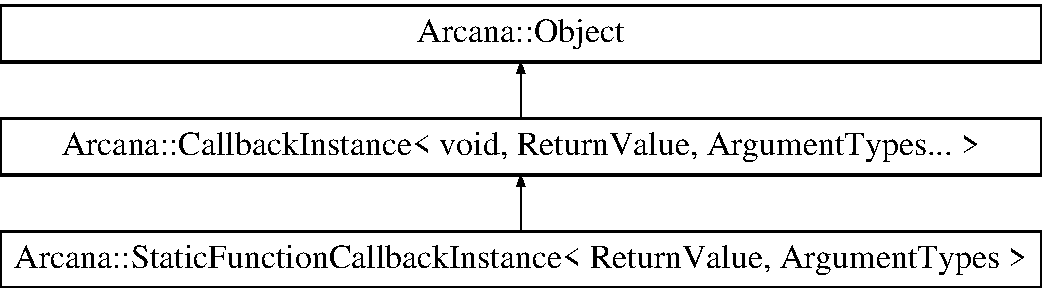
\includegraphics[height=3.000000cm]{class_arcana_1_1_static_function_callback_instance}
\end{center}
\end{figure}
\subsection*{Public Types}
\begin{DoxyCompactItemize}
\item 
\mbox{\Hypertarget{class_arcana_1_1_static_function_callback_instance_a2df756266028ab7af5c4253fbfb230dc}\label{class_arcana_1_1_static_function_callback_instance_a2df756266028ab7af5c4253fbfb230dc}} 
typedef Return\+Value($\ast$ \mbox{\hyperlink{class_arcana_1_1_static_function_callback_instance_a2df756266028ab7af5c4253fbfb230dc}{Callback\+Function}}) (Argument\+Types...)
\begin{DoxyCompactList}\small\item\em Function pointer typedef. \end{DoxyCompactList}\end{DoxyCompactItemize}
\subsection*{Public Member Functions}
\begin{DoxyCompactItemize}
\item 
virtual Return\+Value \mbox{\hyperlink{class_arcana_1_1_static_function_callback_instance_a9666f5e80b24e6e38e5d3766a6a577ac}{execute}} (Argument\+Types \&\&... args) override
\begin{DoxyCompactList}\small\item\em Executes the function. \end{DoxyCompactList}\item 
virtual Return\+Value \mbox{\hyperlink{class_arcana_1_1_static_function_callback_instance_a1e498222014df725ab8dfb737b48c2ef}{execute\+If\+Bound}} (Argument\+Types \&\&... args) override
\begin{DoxyCompactList}\small\item\em Executes the function. \end{DoxyCompactList}\item 
\mbox{\Hypertarget{class_arcana_1_1_static_function_callback_instance_a059c7a2be305f5dbe88a64e5a67a807e}\label{class_arcana_1_1_static_function_callback_instance_a059c7a2be305f5dbe88a64e5a67a807e}} 
virtual bool \mbox{\hyperlink{class_arcana_1_1_static_function_callback_instance_a059c7a2be305f5dbe88a64e5a67a807e}{is\+Bound}} () override
\begin{DoxyCompactList}\small\item\em Returns true if a function pointer is bound. \end{DoxyCompactList}\item 
\mbox{\Hypertarget{class_arcana_1_1_static_function_callback_instance_af2fa2ba277adab6aaabfa78334f57b4a}\label{class_arcana_1_1_static_function_callback_instance_af2fa2ba277adab6aaabfa78334f57b4a}} 
virtual bool \mbox{\hyperlink{class_arcana_1_1_static_function_callback_instance_af2fa2ba277adab6aaabfa78334f57b4a}{is\+Static\+Function}} () const override
\begin{DoxyCompactList}\small\item\em Returns true if a function is a static function. \end{DoxyCompactList}\item 
\mbox{\Hypertarget{class_arcana_1_1_static_function_callback_instance_ae84257a632181a5d942cb61434cc8edc}\label{class_arcana_1_1_static_function_callback_instance_ae84257a632181a5d942cb61434cc8edc}} 
virtual void \mbox{\hyperlink{class_arcana_1_1_static_function_callback_instance_ae84257a632181a5d942cb61434cc8edc}{unbind}} () override
\begin{DoxyCompactList}\small\item\em Sets the object and function pointer members to null. \end{DoxyCompactList}\item 
virtual void \mbox{\hyperlink{class_arcana_1_1_static_function_callback_instance_aaf3de60d3146a2cb8946976d73a6ab2c}{bind}} (\mbox{\hyperlink{class_arcana_1_1_static_function_callback_instance_a2df756266028ab7af5c4253fbfb230dc}{Callback\+Function}} function) override
\begin{DoxyCompactList}\small\item\em Binds a static function pointer to the callback. \end{DoxyCompactList}\end{DoxyCompactItemize}
\subsection*{Public Attributes}
\begin{DoxyCompactItemize}
\item 
\mbox{\Hypertarget{class_arcana_1_1_static_function_callback_instance_aa7d02dca5567209f2c551fbc32f240e4}\label{class_arcana_1_1_static_function_callback_instance_aa7d02dca5567209f2c551fbc32f240e4}} 
\mbox{\hyperlink{class_arcana_1_1_static_function_callback_instance_a2df756266028ab7af5c4253fbfb230dc}{Callback\+Function}} {\bfseries \+\_\+function}
\end{DoxyCompactItemize}


\subsection{Member Function Documentation}
\mbox{\Hypertarget{class_arcana_1_1_static_function_callback_instance_aaf3de60d3146a2cb8946976d73a6ab2c}\label{class_arcana_1_1_static_function_callback_instance_aaf3de60d3146a2cb8946976d73a6ab2c}} 
\index{Arcana\+::\+Static\+Function\+Callback\+Instance@{Arcana\+::\+Static\+Function\+Callback\+Instance}!bind@{bind}}
\index{bind@{bind}!Arcana\+::\+Static\+Function\+Callback\+Instance@{Arcana\+::\+Static\+Function\+Callback\+Instance}}
\subsubsection{\texorpdfstring{bind()}{bind()}}
{\footnotesize\ttfamily template$<$typename Return\+Value , typename... Argument\+Types$>$ \\
virtual void \mbox{\hyperlink{class_arcana_1_1_static_function_callback_instance}{Arcana\+::\+Static\+Function\+Callback\+Instance}}$<$ Return\+Value, Argument\+Types $>$\+::bind (\begin{DoxyParamCaption}\item[{\mbox{\hyperlink{class_arcana_1_1_static_function_callback_instance_a2df756266028ab7af5c4253fbfb230dc}{Callback\+Function}}}]{Callback\+Function }\end{DoxyParamCaption})\hspace{0.3cm}{\ttfamily [inline]}, {\ttfamily [override]}, {\ttfamily [virtual]}}



Binds a static function pointer to the callback. 

The static function must take the arguments specified in the \mbox{\hyperlink{class_arcana_1_1_callback_instance}{Callback\+Instance}} templates. 

Reimplemented from \mbox{\hyperlink{class_arcana_1_1_callback_instance_a6d9b12af5b8a98b782257a7b10eaa7e9}{Arcana\+::\+Callback\+Instance$<$ void, Return\+Value, Argument\+Types... $>$}}.

\mbox{\Hypertarget{class_arcana_1_1_static_function_callback_instance_a9666f5e80b24e6e38e5d3766a6a577ac}\label{class_arcana_1_1_static_function_callback_instance_a9666f5e80b24e6e38e5d3766a6a577ac}} 
\index{Arcana\+::\+Static\+Function\+Callback\+Instance@{Arcana\+::\+Static\+Function\+Callback\+Instance}!execute@{execute}}
\index{execute@{execute}!Arcana\+::\+Static\+Function\+Callback\+Instance@{Arcana\+::\+Static\+Function\+Callback\+Instance}}
\subsubsection{\texorpdfstring{execute()}{execute()}}
{\footnotesize\ttfamily template$<$typename Return\+Value , typename... Argument\+Types$>$ \\
virtual Return\+Value \mbox{\hyperlink{class_arcana_1_1_static_function_callback_instance}{Arcana\+::\+Static\+Function\+Callback\+Instance}}$<$ Return\+Value, Argument\+Types $>$\+::execute (\begin{DoxyParamCaption}\item[{Argument\+Types \&\&...}]{args }\end{DoxyParamCaption})\hspace{0.3cm}{\ttfamily [inline]}, {\ttfamily [override]}, {\ttfamily [virtual]}}



Executes the function. 

An unknown number of arguments can be passed. The argument types must coincide with the initial arguments specified in the template. 

Implements \mbox{\hyperlink{class_arcana_1_1_callback_instance_aa5bd9b4ee2129a0c22a98f7fa1cfc724}{Arcana\+::\+Callback\+Instance$<$ void, Return\+Value, Argument\+Types... $>$}}.

\mbox{\Hypertarget{class_arcana_1_1_static_function_callback_instance_a1e498222014df725ab8dfb737b48c2ef}\label{class_arcana_1_1_static_function_callback_instance_a1e498222014df725ab8dfb737b48c2ef}} 
\index{Arcana\+::\+Static\+Function\+Callback\+Instance@{Arcana\+::\+Static\+Function\+Callback\+Instance}!execute\+If\+Bound@{execute\+If\+Bound}}
\index{execute\+If\+Bound@{execute\+If\+Bound}!Arcana\+::\+Static\+Function\+Callback\+Instance@{Arcana\+::\+Static\+Function\+Callback\+Instance}}
\subsubsection{\texorpdfstring{execute\+If\+Bound()}{executeIfBound()}}
{\footnotesize\ttfamily template$<$typename Return\+Value , typename... Argument\+Types$>$ \\
virtual Return\+Value \mbox{\hyperlink{class_arcana_1_1_static_function_callback_instance}{Arcana\+::\+Static\+Function\+Callback\+Instance}}$<$ Return\+Value, Argument\+Types $>$\+::execute\+If\+Bound (\begin{DoxyParamCaption}\item[{Argument\+Types \&\&...}]{args }\end{DoxyParamCaption})\hspace{0.3cm}{\ttfamily [inline]}, {\ttfamily [override]}, {\ttfamily [virtual]}}



Executes the function. 

An unknown number of arguments can be passed. The argument types must coincide with the initial arguments specified in the template. This method is the same as \mbox{\hyperlink{class_arcana_1_1_static_function_callback_instance_a9666f5e80b24e6e38e5d3766a6a577ac}{execute()}}, but without the assertion. 

Implements \mbox{\hyperlink{class_arcana_1_1_callback_instance_af4aced5d787cabb857931ecd87c3ab50}{Arcana\+::\+Callback\+Instance$<$ void, Return\+Value, Argument\+Types... $>$}}.



The documentation for this class was generated from the following file\+:\begin{DoxyCompactItemize}
\item 
Static\+Function\+Callback\+Instance.\+h\end{DoxyCompactItemize}

\hypertarget{class_arcana_1_1_string}{}\section{Arcana\+:\+:String Class Reference}
\label{class_arcana_1_1_string}\index{Arcana\+::\+String@{Arcana\+::\+String}}


The documentation for this class was generated from the following files\+:\begin{DoxyCompactItemize}
\item 
Arcana\+String.\+h\item 
Arcana\+String.\+cpp\end{DoxyCompactItemize}

\hypertarget{class_arcana_1_1_time}{}\section{Arcana\+:\+:Time Class Reference}
\label{class_arcana_1_1_time}\index{Arcana\+::\+Time@{Arcana\+::\+Time}}


Class for wrapping a time duration.  




{\ttfamily \#include $<$Arcana\+Time.\+h$>$}

\subsection*{Public Member Functions}
\begin{DoxyCompactItemize}
\item 
\mbox{\hyperlink{class_arcana_1_1_time_a5a14897b858a9ab2ee905697981318c9}{Time}} ()
\begin{DoxyCompactList}\small\item\em Default constructor. \end{DoxyCompactList}\item 
\mbox{\hyperlink{class_arcana_1_1_time_a12d30cc17ba7aabd9910fa33c4bf3271}{Time}} (int64 microseconds)
\begin{DoxyCompactList}\small\item\em Int64 constructor. \end{DoxyCompactList}\item 
\mbox{\Hypertarget{class_arcana_1_1_time_aa073ffdc5313b86ac0190bbf71872845}\label{class_arcana_1_1_time_aa073ffdc5313b86ac0190bbf71872845}} 
\mbox{\hyperlink{class_arcana_1_1_time_aa073ffdc5313b86ac0190bbf71872845}{$\sim$\+Time}} ()
\begin{DoxyCompactList}\small\item\em Default destructor. \end{DoxyCompactList}\item 
\mbox{\Hypertarget{class_arcana_1_1_time_a62cfa57729d88885fada52012d8d39e4}\label{class_arcana_1_1_time_a62cfa57729d88885fada52012d8d39e4}} 
int64 \mbox{\hyperlink{class_arcana_1_1_time_a62cfa57729d88885fada52012d8d39e4}{to\+Nanoseconds}} () const
\begin{DoxyCompactList}\small\item\em Returns the time in nanoseconds. \end{DoxyCompactList}\item 
\mbox{\Hypertarget{class_arcana_1_1_time_ae5494b64cfb03356395c7177b1db6ec9}\label{class_arcana_1_1_time_ae5494b64cfb03356395c7177b1db6ec9}} 
int64 \mbox{\hyperlink{class_arcana_1_1_time_ae5494b64cfb03356395c7177b1db6ec9}{to\+Microseconds}} () const
\begin{DoxyCompactList}\small\item\em Returns the time in microseconds. \end{DoxyCompactList}\item 
\mbox{\Hypertarget{class_arcana_1_1_time_a5ec7c36eab957b61bf897c57a6d1a50b}\label{class_arcana_1_1_time_a5ec7c36eab957b61bf897c57a6d1a50b}} 
int32 \mbox{\hyperlink{class_arcana_1_1_time_a5ec7c36eab957b61bf897c57a6d1a50b}{to\+Milliseconds}} () const
\begin{DoxyCompactList}\small\item\em Returns the time in milliseconds. \end{DoxyCompactList}\item 
\mbox{\Hypertarget{class_arcana_1_1_time_a304131c7ca500e1468beb141b1f888cd}\label{class_arcana_1_1_time_a304131c7ca500e1468beb141b1f888cd}} 
double \mbox{\hyperlink{class_arcana_1_1_time_a304131c7ca500e1468beb141b1f888cd}{to\+Seconds}} () const
\begin{DoxyCompactList}\small\item\em Returns the time in seconds. \end{DoxyCompactList}\item 
\mbox{\Hypertarget{class_arcana_1_1_time_a99c3ecaa9a6d786455118f2b963fac81}\label{class_arcana_1_1_time_a99c3ecaa9a6d786455118f2b963fac81}} 
bool \mbox{\hyperlink{class_arcana_1_1_time_a99c3ecaa9a6d786455118f2b963fac81}{is\+Zero}} () const
\begin{DoxyCompactList}\small\item\em Returns true if the time is zero. \end{DoxyCompactList}\end{DoxyCompactItemize}
\subsection*{Static Public Member Functions}
\begin{DoxyCompactItemize}
\item 
\mbox{\Hypertarget{class_arcana_1_1_time_a82db96262751ea46d56f0fc6388efbcf}\label{class_arcana_1_1_time_a82db96262751ea46d56f0fc6388efbcf}} 
static \mbox{\hyperlink{class_arcana_1_1_time}{Time}} \mbox{\hyperlink{class_arcana_1_1_time_a82db96262751ea46d56f0fc6388efbcf}{from\+Nanoseconds}} (int64 nanoseconds)
\begin{DoxyCompactList}\small\item\em Creates a \mbox{\hyperlink{class_arcana_1_1_time}{Time}} object from nanoseconds. \end{DoxyCompactList}\item 
\mbox{\Hypertarget{class_arcana_1_1_time_a95ac577d056c4909dbf4d9cb43c64383}\label{class_arcana_1_1_time_a95ac577d056c4909dbf4d9cb43c64383}} 
static \mbox{\hyperlink{class_arcana_1_1_time}{Time}} \mbox{\hyperlink{class_arcana_1_1_time_a95ac577d056c4909dbf4d9cb43c64383}{from\+Milliseconds}} (int32 milliseconds)
\begin{DoxyCompactList}\small\item\em Creates a \mbox{\hyperlink{class_arcana_1_1_time}{Time}} object from milliseconds. \end{DoxyCompactList}\item 
\mbox{\Hypertarget{class_arcana_1_1_time_ab2e8c472e70a57905da61551d6a5d0e3}\label{class_arcana_1_1_time_ab2e8c472e70a57905da61551d6a5d0e3}} 
static \mbox{\hyperlink{class_arcana_1_1_time}{Time}} \mbox{\hyperlink{class_arcana_1_1_time_ab2e8c472e70a57905da61551d6a5d0e3}{from\+Seconds}} (double seconds)
\begin{DoxyCompactList}\small\item\em Creates a \mbox{\hyperlink{class_arcana_1_1_time}{Time}} object from seconds. \end{DoxyCompactList}\end{DoxyCompactItemize}


\subsection{Detailed Description}
Class for wrapping a time duration. 

Stores the time in microseconds. Provides methods for converting between time units. 

\subsection{Constructor \& Destructor Documentation}
\mbox{\Hypertarget{class_arcana_1_1_time_a5a14897b858a9ab2ee905697981318c9}\label{class_arcana_1_1_time_a5a14897b858a9ab2ee905697981318c9}} 
\index{Arcana\+::\+Time@{Arcana\+::\+Time}!Time@{Time}}
\index{Time@{Time}!Arcana\+::\+Time@{Arcana\+::\+Time}}
\subsubsection{\texorpdfstring{Time()}{Time()}\hspace{0.1cm}{\footnotesize\ttfamily [1/2]}}
{\footnotesize\ttfamily Arcana\+::\+Time\+::\+Time (\begin{DoxyParamCaption}{ }\end{DoxyParamCaption})}



Default constructor. 

Initializes the time to zero. \mbox{\Hypertarget{class_arcana_1_1_time_a12d30cc17ba7aabd9910fa33c4bf3271}\label{class_arcana_1_1_time_a12d30cc17ba7aabd9910fa33c4bf3271}} 
\index{Arcana\+::\+Time@{Arcana\+::\+Time}!Time@{Time}}
\index{Time@{Time}!Arcana\+::\+Time@{Arcana\+::\+Time}}
\subsubsection{\texorpdfstring{Time()}{Time()}\hspace{0.1cm}{\footnotesize\ttfamily [2/2]}}
{\footnotesize\ttfamily Arcana\+::\+Time\+::\+Time (\begin{DoxyParamCaption}\item[{int64}]{microseconds }\end{DoxyParamCaption})}



Int64 constructor. 

Initializes the time in microseconds. 

The documentation for this class was generated from the following files\+:\begin{DoxyCompactItemize}
\item 
Arcana\+Time.\+h\item 
Time.\+cpp\end{DoxyCompactItemize}

\hypertarget{class_arcana_1_1_timeline}{}\section{Arcana\+:\+:Timeline Class Reference}
\label{class_arcana_1_1_timeline}\index{Arcana\+::\+Timeline@{Arcana\+::\+Timeline}}


This class manages a timeline.  




{\ttfamily \#include $<$Timeline.\+h$>$}

Inheritance diagram for Arcana\+:\+:Timeline\+:\begin{figure}[H]
\begin{center}
\leavevmode
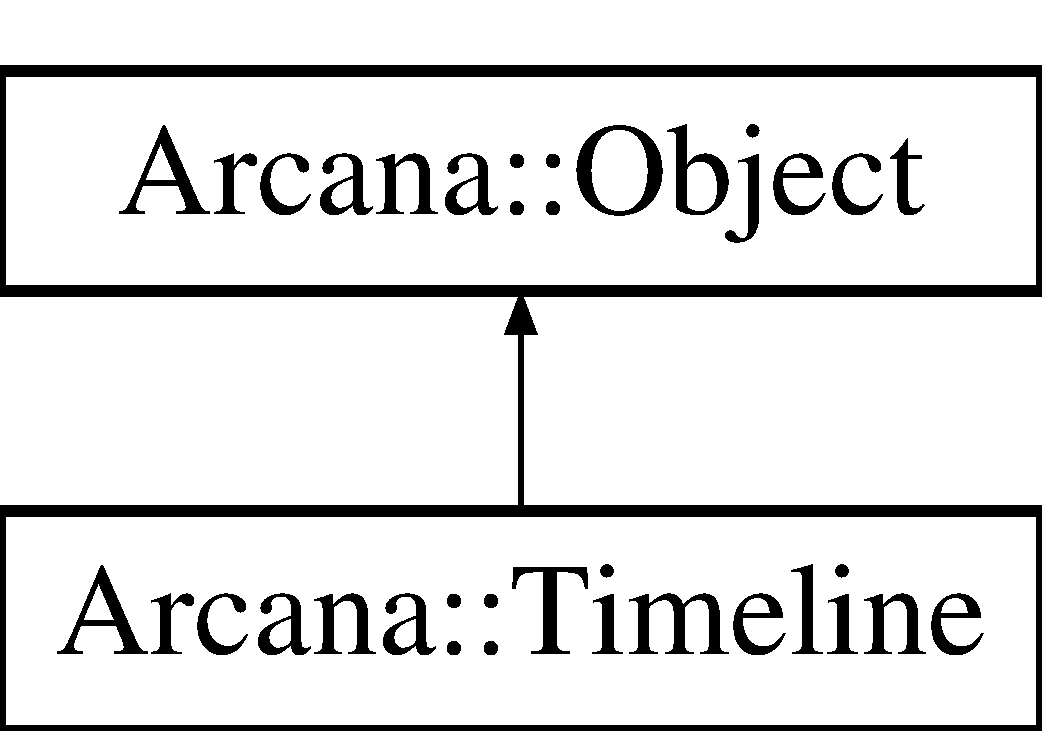
\includegraphics[height=2.000000cm]{class_arcana_1_1_timeline}
\end{center}
\end{figure}
\subsection*{Classes}
\begin{DoxyCompactItemize}
\item 
struct \mbox{\hyperlink{struct_arcana_1_1_timeline_1_1_event_entry}{Event\+Entry}}
\begin{DoxyCompactList}\small\item\em An event entry. \end{DoxyCompactList}\end{DoxyCompactItemize}
\subsection*{Public Types}
\begin{DoxyCompactItemize}
\item 
enum \mbox{\hyperlink{class_arcana_1_1_timeline_ab4605d34e12005cf268ca146751f1eed}{Length\+Mode}} \{ \mbox{\hyperlink{class_arcana_1_1_timeline_ab4605d34e12005cf268ca146751f1eeda392c0af54c9f73e38d8e676605464110}{Timeline\+Length}}, 
\mbox{\hyperlink{class_arcana_1_1_timeline_ab4605d34e12005cf268ca146751f1eedaad8bacad8edb62e39b9972fac10f2cba}{Last\+Key\+Frame}}
 \}
\begin{DoxyCompactList}\small\item\em Length mode enum. \end{DoxyCompactList}\end{DoxyCompactItemize}
\subsection*{Public Member Functions}
\begin{DoxyCompactItemize}
\item 
\mbox{\hyperlink{class_arcana_1_1_timeline_a4a9b19ce9b7480a6816c0476b7fa2330}{Timeline}} ()
\begin{DoxyCompactList}\small\item\em \mbox{\hyperlink{class_arcana_1_1_timeline}{Timeline}} default constructor. \end{DoxyCompactList}\item 
\mbox{\Hypertarget{class_arcana_1_1_timeline_a21dd0ab8ed0aac6c25c4fe604c4a31a5}\label{class_arcana_1_1_timeline_a21dd0ab8ed0aac6c25c4fe604c4a31a5}} 
void \mbox{\hyperlink{class_arcana_1_1_timeline_a21dd0ab8ed0aac6c25c4fe604c4a31a5}{play}} ()
\begin{DoxyCompactList}\small\item\em Starts the timeline. \end{DoxyCompactList}\item 
\mbox{\Hypertarget{class_arcana_1_1_timeline_ad0286df5c28fa561e8222bdc29e9e61b}\label{class_arcana_1_1_timeline_ad0286df5c28fa561e8222bdc29e9e61b}} 
void \mbox{\hyperlink{class_arcana_1_1_timeline_ad0286df5c28fa561e8222bdc29e9e61b}{play\+From\+Start}} ()
\begin{DoxyCompactList}\small\item\em Resets the position to zero and starts the timeline. \end{DoxyCompactList}\item 
\mbox{\Hypertarget{class_arcana_1_1_timeline_a3271fcaccf36add4e09dfa1342749c4d}\label{class_arcana_1_1_timeline_a3271fcaccf36add4e09dfa1342749c4d}} 
void \mbox{\hyperlink{class_arcana_1_1_timeline_a3271fcaccf36add4e09dfa1342749c4d}{reverse}} ()
\begin{DoxyCompactList}\small\item\em Starts the timeline in reverse. \end{DoxyCompactList}\item 
\mbox{\Hypertarget{class_arcana_1_1_timeline_aabdf70e515e2708e1749beb5dece6190}\label{class_arcana_1_1_timeline_aabdf70e515e2708e1749beb5dece6190}} 
void \mbox{\hyperlink{class_arcana_1_1_timeline_aabdf70e515e2708e1749beb5dece6190}{reverse\+From\+End}} ()
\begin{DoxyCompactList}\small\item\em Resets the position to the end and starts the timeline in reverse. \end{DoxyCompactList}\item 
\mbox{\Hypertarget{class_arcana_1_1_timeline_abcefca3d28a1a5ad95fb4e84d980a3de}\label{class_arcana_1_1_timeline_abcefca3d28a1a5ad95fb4e84d980a3de}} 
void \mbox{\hyperlink{class_arcana_1_1_timeline_abcefca3d28a1a5ad95fb4e84d980a3de}{stop}} ()
\begin{DoxyCompactList}\small\item\em Stops the timeline. \end{DoxyCompactList}\item 
\mbox{\Hypertarget{class_arcana_1_1_timeline_ae5b227828f15f1066e30a5341f7923b3}\label{class_arcana_1_1_timeline_ae5b227828f15f1066e30a5341f7923b3}} 
bool \mbox{\hyperlink{class_arcana_1_1_timeline_ae5b227828f15f1066e30a5341f7923b3}{is\+Playing}} () const
\begin{DoxyCompactList}\small\item\em Returns true if the timeline is playing. \end{DoxyCompactList}\item 
\mbox{\Hypertarget{class_arcana_1_1_timeline_a14af7d00e66fe57110340a824295805c}\label{class_arcana_1_1_timeline_a14af7d00e66fe57110340a824295805c}} 
bool \mbox{\hyperlink{class_arcana_1_1_timeline_a14af7d00e66fe57110340a824295805c}{is\+Reversing}} () const
\begin{DoxyCompactList}\small\item\em Returns true if the timeline is reversing. \end{DoxyCompactList}\item 
void \mbox{\hyperlink{class_arcana_1_1_timeline_afba20a0d02f23e9bbf752f6c1a7a589b}{set\+Playback\+Position}} (double position, bool fire\+Events)
\begin{DoxyCompactList}\small\item\em Mutator for the timeline position. \end{DoxyCompactList}\item 
\mbox{\Hypertarget{class_arcana_1_1_timeline_ad144e4650f3b95c5df1608872b586e16}\label{class_arcana_1_1_timeline_ad144e4650f3b95c5df1608872b586e16}} 
double \mbox{\hyperlink{class_arcana_1_1_timeline_ad144e4650f3b95c5df1608872b586e16}{get\+Playback\+Position}} () const
\begin{DoxyCompactList}\small\item\em Accessor for the timeline position. \end{DoxyCompactList}\item 
\mbox{\Hypertarget{class_arcana_1_1_timeline_ab9fb7b10c29cfda510feb40816be971c}\label{class_arcana_1_1_timeline_ab9fb7b10c29cfda510feb40816be971c}} 
void \mbox{\hyperlink{class_arcana_1_1_timeline_ab9fb7b10c29cfda510feb40816be971c}{set\+Looped}} (bool looped)
\begin{DoxyCompactList}\small\item\em Mutator for looping the timeline. \end{DoxyCompactList}\item 
\mbox{\Hypertarget{class_arcana_1_1_timeline_a0acc5055bd1a822e2bc34ecb36f4466c}\label{class_arcana_1_1_timeline_a0acc5055bd1a822e2bc34ecb36f4466c}} 
bool \mbox{\hyperlink{class_arcana_1_1_timeline_a0acc5055bd1a822e2bc34ecb36f4466c}{is\+Looped}} () const
\begin{DoxyCompactList}\small\item\em Returns true if the timeline is looped. \end{DoxyCompactList}\item 
void \mbox{\hyperlink{class_arcana_1_1_timeline_aec6c9fdd12143c467202658b39fb62e8}{set\+Time\+Scale}} (double time\+Scale)
\begin{DoxyCompactList}\small\item\em Mutator for the time scale. \end{DoxyCompactList}\item 
\mbox{\Hypertarget{class_arcana_1_1_timeline_a623bcd9e19e42f2e066431dfc9b37729}\label{class_arcana_1_1_timeline_a623bcd9e19e42f2e066431dfc9b37729}} 
double \mbox{\hyperlink{class_arcana_1_1_timeline_a623bcd9e19e42f2e066431dfc9b37729}{get\+Time\+Scale}} () const
\begin{DoxyCompactList}\small\item\em Accessor for the time scale. \end{DoxyCompactList}\item 
void \mbox{\hyperlink{class_arcana_1_1_timeline_a54c3355a9f97c5173a3b7b0bb5146647}{set\+New\+Time}} (double time)
\begin{DoxyCompactList}\small\item\em Sets the timeline position. \end{DoxyCompactList}\item 
\mbox{\Hypertarget{class_arcana_1_1_timeline_a95c061f715dcfe16c4f3fbe944f01f67}\label{class_arcana_1_1_timeline_a95c061f715dcfe16c4f3fbe944f01f67}} 
void \mbox{\hyperlink{class_arcana_1_1_timeline_a95c061f715dcfe16c4f3fbe944f01f67}{set\+Timeline\+Length}} (double length)
\begin{DoxyCompactList}\small\item\em Sets the timeline length. \end{DoxyCompactList}\item 
\mbox{\Hypertarget{class_arcana_1_1_timeline_a6b7c05ac977edfc48134ef73ad349851}\label{class_arcana_1_1_timeline_a6b7c05ac977edfc48134ef73ad349851}} 
double \mbox{\hyperlink{class_arcana_1_1_timeline_a6b7c05ac977edfc48134ef73ad349851}{get\+Timeline\+Length}} () const
\begin{DoxyCompactList}\small\item\em Accessor for the timeline length. \end{DoxyCompactList}\item 
\mbox{\Hypertarget{class_arcana_1_1_timeline_a00f122bb58c1cfdca6b9cec572944822}\label{class_arcana_1_1_timeline_a00f122bb58c1cfdca6b9cec572944822}} 
void \mbox{\hyperlink{class_arcana_1_1_timeline_a00f122bb58c1cfdca6b9cec572944822}{set\+Timeline\+Length\+Mode}} (\mbox{\hyperlink{class_arcana_1_1_timeline_ab4605d34e12005cf268ca146751f1eed}{Length\+Mode}} mode)
\begin{DoxyCompactList}\small\item\em Sets the timeline length mode. \end{DoxyCompactList}\item 
\mbox{\Hypertarget{class_arcana_1_1_timeline_ac188a005b0c36b4fe35f7e38d7998a07}\label{class_arcana_1_1_timeline_ac188a005b0c36b4fe35f7e38d7998a07}} 
void \mbox{\hyperlink{class_arcana_1_1_timeline_ac188a005b0c36b4fe35f7e38d7998a07}{add\+Event}} (double time, \mbox{\hyperlink{class_arcana_1_1_event}{Event}} event)
\begin{DoxyCompactList}\small\item\em Schedules an \mbox{\hyperlink{class_arcana_1_1_event}{Event}} to be broadcasted at the specified time. \end{DoxyCompactList}\item 
\mbox{\Hypertarget{class_arcana_1_1_timeline_a4de0541fc0f525373f7f1dee707a3548}\label{class_arcana_1_1_timeline_a4de0541fc0f525373f7f1dee707a3548}} 
void \mbox{\hyperlink{class_arcana_1_1_timeline_a4de0541fc0f525373f7f1dee707a3548}{update\+Timeline}} (double delta\+Time)
\begin{DoxyCompactList}\small\item\em Updates the timeline. \end{DoxyCompactList}\item 
void \mbox{\hyperlink{class_arcana_1_1_timeline_acf36a46fcebfed3097b12e2f90ed6ccd}{set\+Event\+Handler}} (\mbox{\hyperlink{class_arcana_1_1_event_handler}{Event\+Handler}} \&event\+Handler)
\begin{DoxyCompactList}\small\item\em Sets the \mbox{\hyperlink{class_arcana_1_1_event_handler}{Event\+Handler}} for this timeline. \end{DoxyCompactList}\item 
\mbox{\Hypertarget{class_arcana_1_1_timeline_a5a973e73ab5f8c4feb69faf1c39047ba}\label{class_arcana_1_1_timeline_a5a973e73ab5f8c4feb69faf1c39047ba}} 
Timeline\+Finished \& \mbox{\hyperlink{class_arcana_1_1_timeline_a5a973e73ab5f8c4feb69faf1c39047ba}{get\+Timeline\+Finished\+Callback}} ()
\begin{DoxyCompactList}\small\item\em Returns a reference to the member function Timeline\+Finished callback. \end{DoxyCompactList}\item 
\mbox{\Hypertarget{class_arcana_1_1_timeline_a05bea86db2489aa9e31d42bd85bb042e}\label{class_arcana_1_1_timeline_a05bea86db2489aa9e31d42bd85bb042e}} 
Timeline\+Finished \& \mbox{\hyperlink{class_arcana_1_1_timeline_a05bea86db2489aa9e31d42bd85bb042e}{get\+Timeline\+Finished\+Callback\+Static}} ()
\begin{DoxyCompactList}\small\item\em Returns a reference to the static function Timeline\+Finished callback. \end{DoxyCompactList}\end{DoxyCompactItemize}


\subsection{Detailed Description}
This class manages a timeline. 

Events can be scheduled at specific times on the timeline. The engine manages a timeline of its own. 

\subsection{Member Enumeration Documentation}
\mbox{\Hypertarget{class_arcana_1_1_timeline_ab4605d34e12005cf268ca146751f1eed}\label{class_arcana_1_1_timeline_ab4605d34e12005cf268ca146751f1eed}} 
\index{Arcana\+::\+Timeline@{Arcana\+::\+Timeline}!Length\+Mode@{Length\+Mode}}
\index{Length\+Mode@{Length\+Mode}!Arcana\+::\+Timeline@{Arcana\+::\+Timeline}}
\subsubsection{\texorpdfstring{Length\+Mode}{LengthMode}}
{\footnotesize\ttfamily enum \mbox{\hyperlink{class_arcana_1_1_timeline_ab4605d34e12005cf268ca146751f1eed}{Arcana\+::\+Timeline\+::\+Length\+Mode}}}



Length mode enum. 

\begin{DoxyEnumFields}{Enumerator}
\raisebox{\heightof{T}}[0pt][0pt]{\index{Timeline\+Length@{Timeline\+Length}!Arcana\+::\+Timeline@{Arcana\+::\+Timeline}}\index{Arcana\+::\+Timeline@{Arcana\+::\+Timeline}!Timeline\+Length@{Timeline\+Length}}}\mbox{\Hypertarget{class_arcana_1_1_timeline_ab4605d34e12005cf268ca146751f1eeda392c0af54c9f73e38d8e676605464110}\label{class_arcana_1_1_timeline_ab4605d34e12005cf268ca146751f1eeda392c0af54c9f73e38d8e676605464110}} 
Timeline\+Length&The timeline stops at a set length. \\
\hline

\raisebox{\heightof{T}}[0pt][0pt]{\index{Last\+Key\+Frame@{Last\+Key\+Frame}!Arcana\+::\+Timeline@{Arcana\+::\+Timeline}}\index{Arcana\+::\+Timeline@{Arcana\+::\+Timeline}!Last\+Key\+Frame@{Last\+Key\+Frame}}}\mbox{\Hypertarget{class_arcana_1_1_timeline_ab4605d34e12005cf268ca146751f1eedaad8bacad8edb62e39b9972fac10f2cba}\label{class_arcana_1_1_timeline_ab4605d34e12005cf268ca146751f1eedaad8bacad8edb62e39b9972fac10f2cba}} 
Last\+Key\+Frame&The timeline stops at the last event keyframe. \\
\hline

\end{DoxyEnumFields}


\subsection{Constructor \& Destructor Documentation}
\mbox{\Hypertarget{class_arcana_1_1_timeline_a4a9b19ce9b7480a6816c0476b7fa2330}\label{class_arcana_1_1_timeline_a4a9b19ce9b7480a6816c0476b7fa2330}} 
\index{Arcana\+::\+Timeline@{Arcana\+::\+Timeline}!Timeline@{Timeline}}
\index{Timeline@{Timeline}!Arcana\+::\+Timeline@{Arcana\+::\+Timeline}}
\subsubsection{\texorpdfstring{Timeline()}{Timeline()}}
{\footnotesize\ttfamily Arcana\+::\+Timeline\+::\+Timeline (\begin{DoxyParamCaption}{ }\end{DoxyParamCaption})}



\mbox{\hyperlink{class_arcana_1_1_timeline}{Timeline}} default constructor. 

Sets length and position to zero. Does not start the timeline! 

\subsection{Member Function Documentation}
\mbox{\Hypertarget{class_arcana_1_1_timeline_acf36a46fcebfed3097b12e2f90ed6ccd}\label{class_arcana_1_1_timeline_acf36a46fcebfed3097b12e2f90ed6ccd}} 
\index{Arcana\+::\+Timeline@{Arcana\+::\+Timeline}!set\+Event\+Handler@{set\+Event\+Handler}}
\index{set\+Event\+Handler@{set\+Event\+Handler}!Arcana\+::\+Timeline@{Arcana\+::\+Timeline}}
\subsubsection{\texorpdfstring{set\+Event\+Handler()}{setEventHandler()}}
{\footnotesize\ttfamily void Arcana\+::\+Timeline\+::set\+Event\+Handler (\begin{DoxyParamCaption}\item[{\mbox{\hyperlink{class_arcana_1_1_event_handler}{Event\+Handler}} \&}]{event\+Handler }\end{DoxyParamCaption})}



Sets the \mbox{\hyperlink{class_arcana_1_1_event_handler}{Event\+Handler}} for this timeline. 

All scheduled events will be broadcasted with this event handler. \mbox{\Hypertarget{class_arcana_1_1_timeline_a54c3355a9f97c5173a3b7b0bb5146647}\label{class_arcana_1_1_timeline_a54c3355a9f97c5173a3b7b0bb5146647}} 
\index{Arcana\+::\+Timeline@{Arcana\+::\+Timeline}!set\+New\+Time@{set\+New\+Time}}
\index{set\+New\+Time@{set\+New\+Time}!Arcana\+::\+Timeline@{Arcana\+::\+Timeline}}
\subsubsection{\texorpdfstring{set\+New\+Time()}{setNewTime()}}
{\footnotesize\ttfamily void Arcana\+::\+Timeline\+::set\+New\+Time (\begin{DoxyParamCaption}\item[{double}]{time }\end{DoxyParamCaption})}



Sets the timeline position. 

Same as set\+Playback\+Position. Doesn\textquotesingle{}t broadcast events. \mbox{\Hypertarget{class_arcana_1_1_timeline_afba20a0d02f23e9bbf752f6c1a7a589b}\label{class_arcana_1_1_timeline_afba20a0d02f23e9bbf752f6c1a7a589b}} 
\index{Arcana\+::\+Timeline@{Arcana\+::\+Timeline}!set\+Playback\+Position@{set\+Playback\+Position}}
\index{set\+Playback\+Position@{set\+Playback\+Position}!Arcana\+::\+Timeline@{Arcana\+::\+Timeline}}
\subsubsection{\texorpdfstring{set\+Playback\+Position()}{setPlaybackPosition()}}
{\footnotesize\ttfamily void Arcana\+::\+Timeline\+::set\+Playback\+Position (\begin{DoxyParamCaption}\item[{double}]{position,  }\item[{bool}]{fire\+Events }\end{DoxyParamCaption})}



Mutator for the timeline position. 

If fire\+Events is \textquotesingle{}true\textquotesingle{} all events scheduled prior to \textquotesingle{}position\textquotesingle{} will be broadcasted. \mbox{\Hypertarget{class_arcana_1_1_timeline_aec6c9fdd12143c467202658b39fb62e8}\label{class_arcana_1_1_timeline_aec6c9fdd12143c467202658b39fb62e8}} 
\index{Arcana\+::\+Timeline@{Arcana\+::\+Timeline}!set\+Time\+Scale@{set\+Time\+Scale}}
\index{set\+Time\+Scale@{set\+Time\+Scale}!Arcana\+::\+Timeline@{Arcana\+::\+Timeline}}
\subsubsection{\texorpdfstring{set\+Time\+Scale()}{setTimeScale()}}
{\footnotesize\ttfamily void Arcana\+::\+Timeline\+::set\+Time\+Scale (\begin{DoxyParamCaption}\item[{double}]{time\+Scale }\end{DoxyParamCaption})}



Mutator for the time scale. 

\mbox{\hyperlink{class_arcana_1_1_time}{Time}} deltas are multiplied by the time scale. 

The documentation for this class was generated from the following files\+:\begin{DoxyCompactItemize}
\item 
Timeline.\+h\item 
Timeline.\+cpp\end{DoxyCompactItemize}

\hypertarget{class_arcana_1_1_timer}{}\section{Arcana\+:\+:Timer Class Reference}
\label{class_arcana_1_1_timer}\index{Arcana\+::\+Timer@{Arcana\+::\+Timer}}


A basic timer.  




{\ttfamily \#include $<$Timer.\+h$>$}

\subsection*{Public Member Functions}
\begin{DoxyCompactItemize}
\item 
\mbox{\Hypertarget{class_arcana_1_1_timer_aed21eb672be57fe13d9cc217be0eab38}\label{class_arcana_1_1_timer_aed21eb672be57fe13d9cc217be0eab38}} 
\mbox{\hyperlink{class_arcana_1_1_timer_aed21eb672be57fe13d9cc217be0eab38}{Timer}} ()
\begin{DoxyCompactList}\small\item\em \mbox{\hyperlink{class_arcana_1_1_timer}{Timer}} default constructor. \end{DoxyCompactList}\item 
\mbox{\Hypertarget{class_arcana_1_1_timer_a2dc493f25fd19b33c81223ff0c8187a9}\label{class_arcana_1_1_timer_a2dc493f25fd19b33c81223ff0c8187a9}} 
\mbox{\hyperlink{class_arcana_1_1_timer_a2dc493f25fd19b33c81223ff0c8187a9}{$\sim$\+Timer}} ()
\begin{DoxyCompactList}\small\item\em \mbox{\hyperlink{class_arcana_1_1_timer}{Timer}} destructor. \end{DoxyCompactList}\item 
\mbox{\Hypertarget{class_arcana_1_1_timer_a7c994a4b608c1585fbb0cc38cea0bcf5}\label{class_arcana_1_1_timer_a7c994a4b608c1585fbb0cc38cea0bcf5}} 
\mbox{\hyperlink{class_arcana_1_1_time}{Time}} \mbox{\hyperlink{class_arcana_1_1_timer_a7c994a4b608c1585fbb0cc38cea0bcf5}{get\+Elapsed\+Time}} () const
\begin{DoxyCompactList}\small\item\em Returns the elapsed time and resets the clock. \end{DoxyCompactList}\item 
\mbox{\Hypertarget{class_arcana_1_1_timer_a35fb2548a0d576c5265da9093c0f18ef}\label{class_arcana_1_1_timer_a35fb2548a0d576c5265da9093c0f18ef}} 
\mbox{\hyperlink{class_arcana_1_1_time}{Time}} \mbox{\hyperlink{class_arcana_1_1_timer_a35fb2548a0d576c5265da9093c0f18ef}{get\+Start\+Time}} ()
\begin{DoxyCompactList}\small\item\em Returns the clock\textquotesingle{}s start time. \end{DoxyCompactList}\item 
\mbox{\Hypertarget{class_arcana_1_1_timer_a4ec8a8a9295d9f45e2c5c7734c64b138}\label{class_arcana_1_1_timer_a4ec8a8a9295d9f45e2c5c7734c64b138}} 
\mbox{\hyperlink{class_arcana_1_1_time}{Time}} \mbox{\hyperlink{class_arcana_1_1_timer_a4ec8a8a9295d9f45e2c5c7734c64b138}{reset}} ()
\begin{DoxyCompactList}\small\item\em Resets the clock. \end{DoxyCompactList}\end{DoxyCompactItemize}


\subsection{Detailed Description}
A basic timer. 

Calculates the elapsed time. 

The documentation for this class was generated from the following files\+:\begin{DoxyCompactItemize}
\item 
Timer.\+h\item 
Timer.\+cpp\end{DoxyCompactItemize}

\hypertarget{class_arcana_1_1_timer_context}{}\section{Arcana\+:\+:Timer\+Context Class Reference}
\label{class_arcana_1_1_timer_context}\index{Arcana\+::\+Timer\+Context@{Arcana\+::\+Timer\+Context}}


Windows timer implementation.  




{\ttfamily \#include $<$Windows\+Timer\+Context.\+h$>$}

\subsection*{Static Public Member Functions}
\begin{DoxyCompactItemize}
\item 
\mbox{\Hypertarget{class_arcana_1_1_timer_context_a8c9e8ebe4e97958c05c1842ceed706ca}\label{class_arcana_1_1_timer_context_a8c9e8ebe4e97958c05c1842ceed706ca}} 
static int64 \mbox{\hyperlink{class_arcana_1_1_timer_context_a8c9e8ebe4e97958c05c1842ceed706ca}{get\+Current\+Time}} ()
\begin{DoxyCompactList}\small\item\em Returns the current time in microseconds. \end{DoxyCompactList}\end{DoxyCompactItemize}


\subsection{Detailed Description}
Windows timer implementation. 

The documentation for this class was generated from the following files\+:\begin{DoxyCompactItemize}
\item 
Windows\+Timer\+Context.\+h\item 
Windows\+Timer\+Context.\+cpp\end{DoxyCompactItemize}

\hypertarget{class_arcana_1_1_type}{}\section{Arcana\+:\+:Type Class Reference}
\label{class_arcana_1_1_type}\index{Arcana\+::\+Type@{Arcana\+::\+Type}}
\subsection*{Public Member Functions}
\begin{DoxyCompactItemize}
\item 
\mbox{\Hypertarget{class_arcana_1_1_type_a38a4eee8130044cec1437519f2bf518b}\label{class_arcana_1_1_type_a38a4eee8130044cec1437519f2bf518b}} 
{\bfseries Type} (int32 type, int64 size, std\+::string name, std\+::string display\+Name)
\item 
\mbox{\Hypertarget{class_arcana_1_1_type_a9c033c3cfc4c1e43bbe11f1c92be8e4e}\label{class_arcana_1_1_type_a9c033c3cfc4c1e43bbe11f1c92be8e4e}} 
bool {\bfseries operator==} (const \mbox{\hyperlink{class_arcana_1_1_type}{Type}} \&type) const
\end{DoxyCompactItemize}
\subsection*{Public Attributes}
\begin{DoxyCompactItemize}
\item 
\mbox{\Hypertarget{class_arcana_1_1_type_acabd0a0701aab3efb922588737145d89}\label{class_arcana_1_1_type_acabd0a0701aab3efb922588737145d89}} 
int32 {\bfseries id}
\item 
\mbox{\Hypertarget{class_arcana_1_1_type_a51104120a9fe0b8fbce158ccd571fb54}\label{class_arcana_1_1_type_a51104120a9fe0b8fbce158ccd571fb54}} 
int64 {\bfseries size}
\item 
\mbox{\Hypertarget{class_arcana_1_1_type_a90be1f6e814fb0f840c1d8e27bcdce66}\label{class_arcana_1_1_type_a90be1f6e814fb0f840c1d8e27bcdce66}} 
std\+::string {\bfseries name}
\item 
\mbox{\Hypertarget{class_arcana_1_1_type_a6b16b11f7ea9ddc03e4b26a0227373ae}\label{class_arcana_1_1_type_a6b16b11f7ea9ddc03e4b26a0227373ae}} 
std\+::string {\bfseries display\+Name}
\end{DoxyCompactItemize}


The documentation for this class was generated from the following file\+:\begin{DoxyCompactItemize}
\item 
Types.\+h\end{DoxyCompactItemize}

\hypertarget{class_arcana_1_1_types}{}\section{Arcana\+:\+:Types Class Reference}
\label{class_arcana_1_1_types}\index{Arcana\+::\+Types@{Arcana\+::\+Types}}
\subsection*{Static Public Member Functions}
\begin{DoxyCompactItemize}
\item 
\mbox{\Hypertarget{class_arcana_1_1_types_a0939fc459ad6a4e9f45908c2b261b3eb}\label{class_arcana_1_1_types_a0939fc459ad6a4e9f45908c2b261b3eb}} 
static \mbox{\hyperlink{class_arcana_1_1_type}{Type}} {\bfseries parse\+Type\+From\+String} (const std\+::string \&type)
\item 
\mbox{\Hypertarget{class_arcana_1_1_types_a4531ff815c987672c6bc83363a247b74}\label{class_arcana_1_1_types_a4531ff815c987672c6bc83363a247b74}} 
static void {\bfseries register\+Type} (int64 size, std\+::string name, std\+::string display\+Name)
\end{DoxyCompactItemize}
\subsection*{Static Public Attributes}
\begin{DoxyCompactItemize}
\item 
\mbox{\Hypertarget{class_arcana_1_1_types_a9f3eec1163e2931ed87aed5e7b847aa5}\label{class_arcana_1_1_types_a9f3eec1163e2931ed87aed5e7b847aa5}} 
static const \mbox{\hyperlink{class_arcana_1_1_type}{Type}} {\bfseries Error\+Type} = \mbox{\hyperlink{class_arcana_1_1_type}{Type}}(Unknown\+Type, -\/1, \char`\"{}error\+\_\+type\char`\"{}, \char`\"{}Error \mbox{\hyperlink{class_arcana_1_1_type}{Type}}\char`\"{})
\item 
\mbox{\Hypertarget{class_arcana_1_1_types_a77949f4b6273c0b012bf2c3928ffce95}\label{class_arcana_1_1_types_a77949f4b6273c0b012bf2c3928ffce95}} 
static const \mbox{\hyperlink{class_arcana_1_1_type}{Type}} {\bfseries Uint8} = \mbox{\hyperlink{class_arcana_1_1_type}{Type}}(Type\+Name\+::\+Uint8, 1, \char`\"{}uint8\char`\"{}, \char`\"{}8-\/bit Unsigned Integer\char`\"{})
\item 
\mbox{\Hypertarget{class_arcana_1_1_types_a65012cc73a88ba8c577901fb864b65f9}\label{class_arcana_1_1_types_a65012cc73a88ba8c577901fb864b65f9}} 
static const \mbox{\hyperlink{class_arcana_1_1_type}{Type}} {\bfseries Uint16} = \mbox{\hyperlink{class_arcana_1_1_type}{Type}}(Type\+Name\+::\+Uint16, 2, \char`\"{}uint16\char`\"{}, \char`\"{}16-\/bit Unsigned Integer\char`\"{})
\item 
\mbox{\Hypertarget{class_arcana_1_1_types_a2a4ef23dde14a315f1a377790cd71cde}\label{class_arcana_1_1_types_a2a4ef23dde14a315f1a377790cd71cde}} 
static const \mbox{\hyperlink{class_arcana_1_1_type}{Type}} {\bfseries Uint32} = \mbox{\hyperlink{class_arcana_1_1_type}{Type}}(Type\+Name\+::\+Uint32, 4, \char`\"{}uint32\char`\"{}, \char`\"{}32-\/bit Unsigned Integer\char`\"{})
\item 
\mbox{\Hypertarget{class_arcana_1_1_types_adbc832e4fa40ea7b507bc4a1814b4168}\label{class_arcana_1_1_types_adbc832e4fa40ea7b507bc4a1814b4168}} 
static const \mbox{\hyperlink{class_arcana_1_1_type}{Type}} {\bfseries Uint64} = \mbox{\hyperlink{class_arcana_1_1_type}{Type}}(Type\+Name\+::\+Uint64, 8, \char`\"{}uint64\char`\"{}, \char`\"{}64-\/bit Unsigned Integer\char`\"{})
\item 
\mbox{\Hypertarget{class_arcana_1_1_types_a354530c3a8ddce67f62a095777082ec9}\label{class_arcana_1_1_types_a354530c3a8ddce67f62a095777082ec9}} 
static const \mbox{\hyperlink{class_arcana_1_1_type}{Type}} {\bfseries Int8} = \mbox{\hyperlink{class_arcana_1_1_type}{Type}}(Type\+Name\+::\+Int8, 1, \char`\"{}int8\char`\"{}, \char`\"{}8-\/bit Integer\char`\"{})
\item 
\mbox{\Hypertarget{class_arcana_1_1_types_a6022cc2b4ef06dec700d0266745c5356}\label{class_arcana_1_1_types_a6022cc2b4ef06dec700d0266745c5356}} 
static const \mbox{\hyperlink{class_arcana_1_1_type}{Type}} {\bfseries Int16} = \mbox{\hyperlink{class_arcana_1_1_type}{Type}}(Type\+Name\+::\+Int16, 2, \char`\"{}int16\char`\"{}, \char`\"{}16-\/bit Integer\char`\"{})
\item 
\mbox{\Hypertarget{class_arcana_1_1_types_a5f94602ba364e6184b78e19145bb921d}\label{class_arcana_1_1_types_a5f94602ba364e6184b78e19145bb921d}} 
static const \mbox{\hyperlink{class_arcana_1_1_type}{Type}} {\bfseries Int32} = \mbox{\hyperlink{class_arcana_1_1_type}{Type}}(Type\+Name\+::\+Int32, 4, \char`\"{}int32\char`\"{}, \char`\"{}32-\/bit Integer\char`\"{})
\item 
\mbox{\Hypertarget{class_arcana_1_1_types_a376799e4dac8cda83124e2d15e0b4c68}\label{class_arcana_1_1_types_a376799e4dac8cda83124e2d15e0b4c68}} 
static const \mbox{\hyperlink{class_arcana_1_1_type}{Type}} {\bfseries Int64} = \mbox{\hyperlink{class_arcana_1_1_type}{Type}}(Type\+Name\+::\+Int64, 8, \char`\"{}int64\char`\"{}, \char`\"{}64-\/bit Integer\char`\"{})
\item 
\mbox{\Hypertarget{class_arcana_1_1_types_a18d5fbe24be4a3e5c4619147c8bf7352}\label{class_arcana_1_1_types_a18d5fbe24be4a3e5c4619147c8bf7352}} 
static const \mbox{\hyperlink{class_arcana_1_1_type}{Type}} {\bfseries Float} = \mbox{\hyperlink{class_arcana_1_1_type}{Type}}(Type\+Name\+::\+Float, 4, \char`\"{}float\char`\"{}, \char`\"{}32-\/bit Floating Point\char`\"{})
\item 
\mbox{\Hypertarget{class_arcana_1_1_types_a57c098ffdb6f98b28c139cc59e9c6139}\label{class_arcana_1_1_types_a57c098ffdb6f98b28c139cc59e9c6139}} 
static const \mbox{\hyperlink{class_arcana_1_1_type}{Type}} {\bfseries Double} = \mbox{\hyperlink{class_arcana_1_1_type}{Type}}(Type\+Name\+::\+Double, 8, \char`\"{}double\char`\"{}, \char`\"{}64-\/bit Floating Point\char`\"{})
\item 
\mbox{\Hypertarget{class_arcana_1_1_types_ab1e5105ed1caec42d68e2385bd67ad03}\label{class_arcana_1_1_types_ab1e5105ed1caec42d68e2385bd67ad03}} 
static const \mbox{\hyperlink{class_arcana_1_1_type}{Type}} {\bfseries Boolean} = \mbox{\hyperlink{class_arcana_1_1_type}{Type}}(Type\+Name\+::\+Boolean, 1, \char`\"{}bool\char`\"{}, \char`\"{}Boolean\char`\"{})
\item 
\mbox{\Hypertarget{class_arcana_1_1_types_a9d99d96412d7803d0fddce6c028737dd}\label{class_arcana_1_1_types_a9d99d96412d7803d0fddce6c028737dd}} 
static const \mbox{\hyperlink{class_arcana_1_1_type}{Type}} {\bfseries String} = \mbox{\hyperlink{class_arcana_1_1_type}{Type}}(Type\+Name\+::\+String, 8, \char`\"{}string\char`\"{}, \char`\"{}\mbox{\hyperlink{class_arcana_1_1_string}{String}}\char`\"{})
\item 
\mbox{\Hypertarget{class_arcana_1_1_types_ac167a518c23fc8abd607e88a1eeafdca}\label{class_arcana_1_1_types_ac167a518c23fc8abd607e88a1eeafdca}} 
static const \mbox{\hyperlink{class_arcana_1_1_type}{Type}} {\bfseries Vec2f} = \mbox{\hyperlink{class_arcana_1_1_type}{Type}}(Type\+Name\+::\+Vec2f, 8, \char`\"{}vec2f\char`\"{}, \char`\"{}2d Float Vector\char`\"{})
\item 
\mbox{\Hypertarget{class_arcana_1_1_types_a928d9ae7771928aaf035d4fa4fd61b13}\label{class_arcana_1_1_types_a928d9ae7771928aaf035d4fa4fd61b13}} 
static const \mbox{\hyperlink{class_arcana_1_1_type}{Type}} {\bfseries Vec3f} = \mbox{\hyperlink{class_arcana_1_1_type}{Type}}(Type\+Name\+::\+Vec3f, 12, \char`\"{}vec3f\char`\"{}, \char`\"{}3d Float Vector\char`\"{})
\item 
\mbox{\Hypertarget{class_arcana_1_1_types_a602933ed17ef481eb05f344863f3490a}\label{class_arcana_1_1_types_a602933ed17ef481eb05f344863f3490a}} 
static const \mbox{\hyperlink{class_arcana_1_1_type}{Type}} {\bfseries Vec4f} = \mbox{\hyperlink{class_arcana_1_1_type}{Type}}(Type\+Name\+::\+Vec4f, 16, \char`\"{}vec4f\char`\"{}, \char`\"{}4d Float Vector\char`\"{})
\item 
\mbox{\Hypertarget{class_arcana_1_1_types_acd32feaceaaa601d7cce05939c172c40}\label{class_arcana_1_1_types_acd32feaceaaa601d7cce05939c172c40}} 
static const \mbox{\hyperlink{class_arcana_1_1_type}{Type}} {\bfseries Vec2i} = \mbox{\hyperlink{class_arcana_1_1_type}{Type}}(Type\+Name\+::\+Vec2i, 8, \char`\"{}vec2i\char`\"{}, \char`\"{}2d Integer Vector\char`\"{})
\item 
\mbox{\Hypertarget{class_arcana_1_1_types_abfae9e702eecc86cff52a70312d4d1d5}\label{class_arcana_1_1_types_abfae9e702eecc86cff52a70312d4d1d5}} 
static const \mbox{\hyperlink{class_arcana_1_1_type}{Type}} {\bfseries Vec3i} = \mbox{\hyperlink{class_arcana_1_1_type}{Type}}(Type\+Name\+::\+Vec3i, 12, \char`\"{}vec3i\char`\"{}, \char`\"{}3d Integer Vector\char`\"{})
\item 
\mbox{\Hypertarget{class_arcana_1_1_types_ab180e12bae8f9f6d54182b684e610f83}\label{class_arcana_1_1_types_ab180e12bae8f9f6d54182b684e610f83}} 
static const \mbox{\hyperlink{class_arcana_1_1_type}{Type}} {\bfseries Vec4i} = \mbox{\hyperlink{class_arcana_1_1_type}{Type}}(Type\+Name\+::\+Vec4i, 16, \char`\"{}vec4i\char`\"{}, \char`\"{}4d Integer Vector\char`\"{})
\item 
\mbox{\Hypertarget{class_arcana_1_1_types_a887cb56bdfddec4402b94538e30a7e8b}\label{class_arcana_1_1_types_a887cb56bdfddec4402b94538e30a7e8b}} 
static const \mbox{\hyperlink{class_arcana_1_1_type}{Type}} {\bfseries Vec2d} = \mbox{\hyperlink{class_arcana_1_1_type}{Type}}(Type\+Name\+::\+Vec2d, 16, \char`\"{}vec2d\char`\"{}, \char`\"{}2d Double Vector\char`\"{})
\item 
\mbox{\Hypertarget{class_arcana_1_1_types_a82c3f63447bac2cf6d8b1640f051442f}\label{class_arcana_1_1_types_a82c3f63447bac2cf6d8b1640f051442f}} 
static const \mbox{\hyperlink{class_arcana_1_1_type}{Type}} {\bfseries Vec3d} = \mbox{\hyperlink{class_arcana_1_1_type}{Type}}(Type\+Name\+::\+Vec3d, 24, \char`\"{}vec3d\char`\"{}, \char`\"{}3d Double Vector\char`\"{})
\item 
\mbox{\Hypertarget{class_arcana_1_1_types_a15bd4ce7176fa1182883b3e1cd5fbfd1}\label{class_arcana_1_1_types_a15bd4ce7176fa1182883b3e1cd5fbfd1}} 
static const \mbox{\hyperlink{class_arcana_1_1_type}{Type}} {\bfseries Vec4d} = \mbox{\hyperlink{class_arcana_1_1_type}{Type}}(Type\+Name\+::\+Vec4d, 32, \char`\"{}vec4d\char`\"{}, \char`\"{}4d Double Vector\char`\"{})
\end{DoxyCompactItemize}


The documentation for this class was generated from the following files\+:\begin{DoxyCompactItemize}
\item 
Types.\+h\item 
Types.\+cpp\end{DoxyCompactItemize}

\hypertarget{struct_arcana_1_1_type_traits}{}\section{Arcana\+:\+:Type\+Traits$<$ T $>$ Struct Template Reference}
\label{struct_arcana_1_1_type_traits}\index{Arcana\+::\+Type\+Traits$<$ T $>$@{Arcana\+::\+Type\+Traits$<$ T $>$}}
Inheritance diagram for Arcana\+:\+:Type\+Traits$<$ T $>$\+:\begin{figure}[H]
\begin{center}
\leavevmode
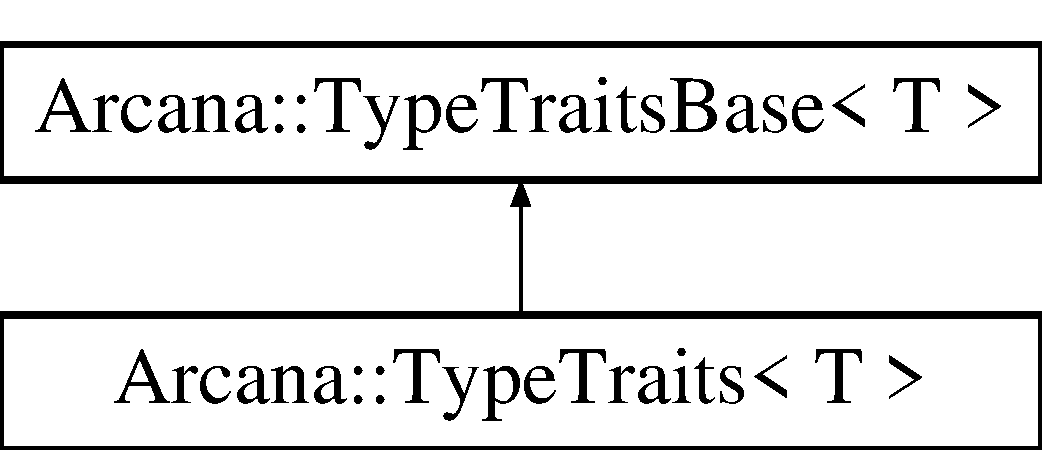
\includegraphics[height=2.000000cm]{struct_arcana_1_1_type_traits}
\end{center}
\end{figure}
\subsection*{Additional Inherited Members}


The documentation for this struct was generated from the following file\+:\begin{DoxyCompactItemize}
\item 
Type\+Traits.\+h\end{DoxyCompactItemize}

\hypertarget{struct_arcana_1_1_type_traits_base}{}\section{Arcana\+:\+:Type\+Traits\+Base$<$ T $>$ Struct Template Reference}
\label{struct_arcana_1_1_type_traits_base}\index{Arcana\+::\+Type\+Traits\+Base$<$ T $>$@{Arcana\+::\+Type\+Traits\+Base$<$ T $>$}}
Inheritance diagram for Arcana\+:\+:Type\+Traits\+Base$<$ T $>$\+:\begin{figure}[H]
\begin{center}
\leavevmode
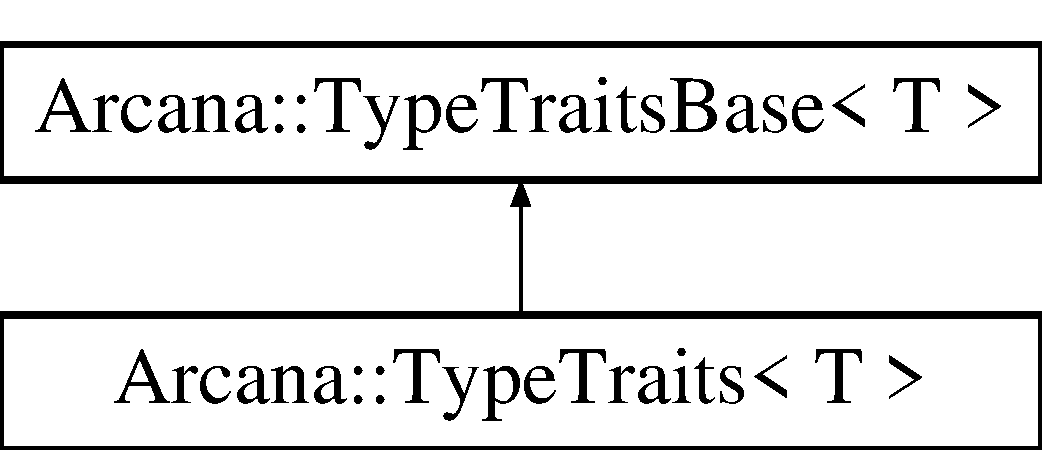
\includegraphics[height=2.000000cm]{struct_arcana_1_1_type_traits_base}
\end{center}
\end{figure}
\subsection*{Public Types}
\begin{DoxyCompactItemize}
\item 
\mbox{\Hypertarget{struct_arcana_1_1_type_traits_base_a3e4718376ed114fd1b82783f373eb111}\label{struct_arcana_1_1_type_traits_base_a3e4718376ed114fd1b82783f373eb111}} 
enum \{ {\bfseries Needs\+Copy\+Constructor} = !std\+:\+:is\+\_\+trivially\+\_\+copyable$<$T$>$\+:\+:value \&\& !std\+:\+:is\+\_\+pod$<$T$>$\+:\+:value \&\& !std\+:\+:is\+\_\+pod$<$T$>$\+:\+:value
 \}
\item 
\mbox{\Hypertarget{struct_arcana_1_1_type_traits_base_a15a07b77815712391596d889800decf7}\label{struct_arcana_1_1_type_traits_base_a15a07b77815712391596d889800decf7}} 
enum \{ {\bfseries Needs\+Copy\+Assignment} = !std\+:\+:is\+\_\+trivially\+\_\+assignable$<$T, T$>$\+:\+:value \&\& !std\+:\+:is\+\_\+pod$<$T$>$\+:\+:value
 \}
\item 
\mbox{\Hypertarget{struct_arcana_1_1_type_traits_base_ae38cddd33259f6c95d67bec6e50b97c4}\label{struct_arcana_1_1_type_traits_base_ae38cddd33259f6c95d67bec6e50b97c4}} 
enum \{ {\bfseries Needs\+Move\+Constructor} = Needs\+Copy\+Constructor
 \}
\item 
\mbox{\Hypertarget{struct_arcana_1_1_type_traits_base_a927fa69db6026ee193a635bec0a3829e}\label{struct_arcana_1_1_type_traits_base_a927fa69db6026ee193a635bec0a3829e}} 
enum \{ {\bfseries Needs\+Move\+Assignment} = Needs\+Copy\+Assignment
 \}
\item 
\mbox{\Hypertarget{struct_arcana_1_1_type_traits_base_a4895060b576fd5f7cc810fa1e2594e4e}\label{struct_arcana_1_1_type_traits_base_a4895060b576fd5f7cc810fa1e2594e4e}} 
enum \{ {\bfseries Needs\+Destructor} = !std\+:\+:is\+\_\+trivially\+\_\+destructible$<$T$>$\+:\+:value \&\& !std\+:\+:is\+\_\+pod$<$T$>$\+:\+:value
 \}
\item 
\mbox{\Hypertarget{struct_arcana_1_1_type_traits_base_a838078202a44d4fd2d4d1610d08070dd}\label{struct_arcana_1_1_type_traits_base_a838078202a44d4fd2d4d1610d08070dd}} 
enum \{ {\bfseries Is\+Bytewise\+Comparable} = std\+:\+:is\+\_\+enum$<$T$>$\+:\+:value $\vert$$\vert$ std\+:\+:is\+\_\+arithmetic$<$T$>$\+:\+:value $\vert$$\vert$ std\+:\+:is\+\_\+pointer$<$T$>$\+:\+:value
 \}
\item 
\mbox{\Hypertarget{struct_arcana_1_1_type_traits_base_a4aed896bc8ddf057e6a521673666fb5b}\label{struct_arcana_1_1_type_traits_base_a4aed896bc8ddf057e6a521673666fb5b}} 
enum \{ {\bfseries Is\+Zero\+Construct\+Type} = Is\+Bytewise\+Comparable
 \}
\end{DoxyCompactItemize}


The documentation for this struct was generated from the following file\+:\begin{DoxyCompactItemize}
\item 
Type\+Traits.\+h\end{DoxyCompactItemize}

\hypertarget{struct_arcana_1_1_memory_allocator_1_1_unknown_type}{}\section{Arcana\+:\+:Memory\+Allocator\+:\+:Unknown\+Type Struct Reference}
\label{struct_arcana_1_1_memory_allocator_1_1_unknown_type}\index{Arcana\+::\+Memory\+Allocator\+::\+Unknown\+Type@{Arcana\+::\+Memory\+Allocator\+::\+Unknown\+Type}}


The documentation for this struct was generated from the following file\+:\begin{DoxyCompactItemize}
\item 
Memory\+Allocator.\+h\end{DoxyCompactItemize}

\hypertarget{class_arcana_1_1_window_closed_event}{}\section{Arcana\+:\+:Window\+Closed\+Event Class Reference}
\label{class_arcana_1_1_window_closed_event}\index{Arcana\+::\+Window\+Closed\+Event@{Arcana\+::\+Window\+Closed\+Event}}


\mbox{\hyperlink{class_arcana_1_1_event}{Event}} broadcasted on window close.  




{\ttfamily \#include $<$No\+Data\+Events.\+h$>$}

Inheritance diagram for Arcana\+:\+:Window\+Closed\+Event\+:\begin{figure}[H]
\begin{center}
\leavevmode
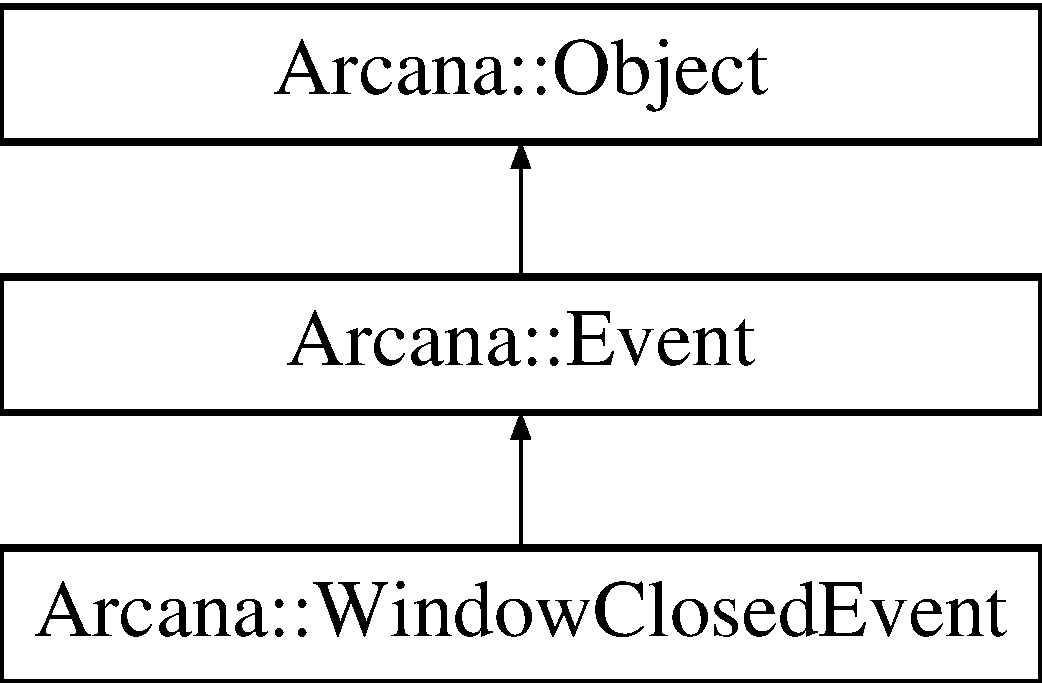
\includegraphics[height=3.000000cm]{class_arcana_1_1_window_closed_event}
\end{center}
\end{figure}
\subsection*{Public Member Functions}
\begin{DoxyCompactItemize}
\item 
\mbox{\Hypertarget{class_arcana_1_1_window_closed_event_aa52319ea28c47ae5ec436666074be8f3}\label{class_arcana_1_1_window_closed_event_aa52319ea28c47ae5ec436666074be8f3}} 
\mbox{\hyperlink{class_arcana_1_1_window_closed_event_aa52319ea28c47ae5ec436666074be8f3}{Window\+Closed\+Event}} ()
\begin{DoxyCompactList}\small\item\em \mbox{\hyperlink{class_arcana_1_1_window_closed_event}{Window\+Closed\+Event}} default constructor. \end{DoxyCompactList}\item 
\mbox{\Hypertarget{class_arcana_1_1_window_closed_event_a80ae09b50ce88ce3c7c9884edb220e86}\label{class_arcana_1_1_window_closed_event_a80ae09b50ce88ce3c7c9884edb220e86}} 
\mbox{\hyperlink{class_arcana_1_1_window_closed_event_a80ae09b50ce88ce3c7c9884edb220e86}{$\sim$\+Window\+Closed\+Event}} ()
\begin{DoxyCompactList}\small\item\em \mbox{\hyperlink{class_arcana_1_1_window_closed_event}{Window\+Closed\+Event}} destructor. \end{DoxyCompactList}\end{DoxyCompactItemize}


\subsection{Detailed Description}
\mbox{\hyperlink{class_arcana_1_1_event}{Event}} broadcasted on window close. 

\mbox{\hyperlink{class_arcana_1_1_window_closed_event}{Window\+Closed\+Event}} have and event id of 3. 

The documentation for this class was generated from the following file\+:\begin{DoxyCompactItemize}
\item 
No\+Data\+Events.\+h\end{DoxyCompactItemize}

%--- End generated contents ---

% Index
\backmatter
\newpage
\phantomsection
\clearemptydoublepage
\addcontentsline{toc}{chapter}{Index}
\printindex

\end{document}
